\documentclass[12pt]{report}
\usepackage[utf8]{inputenc}
\usepackage{graphicx}
\graphicspath{ {images/} }
\usepackage{amssymb}
\usepackage{mathtools}
\usepackage{setspace}
\usepackage{fourier, erewhon, cabin}
\usepackage[english]{babel}
\usepackage{float}
\usepackage{titletoc}
\usepackage{relsize}
%\usepackage[margin=1.25in]{geometry}
\usepackage{lipsum}
\usepackage[top=1.5in, left=1.25in, bottom=1.75in, right=1.25in]{geometry}
\usepackage{titlesec}
\usepackage[toc,page]{appendix}
\usepackage{tocloft}
\usepackage{comment}
\usepackage{listings}
\usepackage{geometry}
\usepackage{xcolor}
\usepackage{blindtext}

\definecolor{mGreen}{rgb}{0,0.6,0}
\definecolor{mGray}{rgb}{0.5,0.5,0.5}
\definecolor{mPurple}{rgb}{0.58,0,0.82}
\definecolor{backgroundColour}{rgb}{0.95,0.95,0.92}

\lstset{
	language=Matlab,
	basicstyle=\ttfamily,
	backgroundcolor=\color{lightgray!25},
	breaklines=true,
	columns=fullflexible,
	frame=single,
	commentstyle=\color{teal},
	identifierstyle=\textbf,
	keywordstyle=\color{magenta},
	numbers=left,
	numberstyle=\footnotesize\sffamily,
	showstringspaces=false
}

\titleformat{\chapter}[display]
{\normalfont\huge\bfseries\centering}{\centering\chaptertitlename\ \thechapter}{15pt}{\huge}
\titlespacing*{\chapter} 
{0pt}{15pt}{15pt}

\addto\captionsenglish{\renewcommand*\contentsname{\centerline{Table of contents}}}

\graphicspath{{C:/Users/User/OneDrive - Seattle University/Documents/Latex/Dissertation/Figures}}

\newcommand\listappendixname{List of Appendices}
\newcommand\appcaption[1]{%
	\addcontentsline{app}{chapter}{#1}}
\makeatletter
\newcommand\listofappendices{%
	\chapter*{\listappendixname}\@starttoc{app}}
\makeatother
	
\newcommand\tab[1][1cm]{\hspace*{#1}}
\renewcommand*\contentsname{Table of Contents}
\renewcommand{\contentsname}{\centering Contents}
\newcommand\Chapter[2]{\chapter
	[#1\hfil\hbox{}\protect\linebreak{\itshape#2}]%
	{#1\\[2ex]\Large\itshape#2}%
}
\newlength{\bracewidth}

\newcommand{\myunderbrace}[2]{\settowidth{\bracewidth}{$#1$}#1\hspace*{-1\bracewidth}\smash{\underbrace{\makebox{\phantom{$#1$}}}_{#2}}}

%\begin{comment}
\renewcommand{\cftchapdotsep}{\cftdotsep} % dots after chapter entries
\setlength{\cftchapnumwidth}{8em} % increase space for chapter numbers
\renewcommand{\cftchappresnum}{CHAPTER } % put this before chapter numbers

 


\begin{document}
		
	\pagestyle{empty}
	
	\begin{titlepage}
	
	\begin{center}
		
		\vspace*{1cm}
		
		\textbf{Real-Time Feedback for Etch Rate and Sidewall Profile
			Control in Reactive Ion Etching}
		
		
		\vspace{3cm}
		
		by
		
		\vspace{0.5cm}
		
		\textbf{Brian Andrew Rashap}
		
		\vfill
		
		A dissertation submitted in partial fulfillment\\
		of the requirements for the degree of\\
		Doctor of Philosophy\\
		(Electrical Engineering: Systems)\\
		in The University of Michigan\\
		1995
		\\
		
		\vspace{0.8cm}
		
	\end{center}
	
	Doctoral Committee:\\
	\tab Associate Professor James S. Freudenberg, Chair\\
	\tab Professor Jessy W. Grizzle\\
	\tab Professor Pramod P. Khargonekar\\
	\tab Associate Professor Fred L. Terry, Jr.\\
	\tab Research Scientist Michael E. Elta\\
	
	\thispagestyle{empty}
\end{titlepage}
		
	\pagenumbering{roman}
	\stepcounter{page}
	
	\addcontentsline{toc}{chapter}{DEDICATION}
\chapter*{}


	
\vspace*{\fill}
	
	\begin{center}
			
			To my mother, father and brother\\
			for their unconditional support of\\
			all of my endeavors.\\
			
	\end{center}
	
\vspace*{\fill}

\clearpage
	
	
	
	\newpage
	
	
\addcontentsline{toc}{chapter}{ACKNOWLEDGMENTS}
\chapter*{ACKNOWLEDGMENTS}

\setstretch{1.5}

\tab This dissertation would not have been possible without the assistance of many people. I apologize in advance if I inadvertently forget to mention anyone.

I would like to begin by thanking my advisor, Professor Jim Freudenberg. Jim was the perfect advisor for me, i.e., most of the time he left me alone so that I could get work done, but he was always available when I needed his guidance. I am really going miss stopping by his office for our late night chats.

I would like to especially thank my dissertation committee: Professors Jessy Grizzle,Pramod Khargonekar, Fred Terry, and Dr. Michael Elta. I could not have asked for a better group of individuals to guide me over the years. They have been great teachers, both inside and outside of the class room, and great friends. I would also like to thank Dr. Martin Giles for his guidance in developing models and simulations for the etching process.

There are a number of people without whose help this research would not have been possible. I would like to thank Keith, Jim and Terry for all their assistance in wafer processing and equipment maintenance. I would especially like to thank Jeff for serving unofficially as my cleanroom mentor. Jeff has taught me most of what I know about running and maintaining semiconductor processing equipment. His guidance has been as valuable to me as that of my dissertation committee. I would also like to thank Don, Chuck, Hugh, Laura, Liz, and Jon for all they have done in maintaining the computers that I have relied on during this research.

I have been very lucky to have the opportunity to work with a group of talented students during my years at the University of Michigan. I want to thank Courtney, Tyrone B., Tyrone V., Pete H., Pete K., Oliver, Anna, Meera, Manish, Steve T., Bill and A1 for being great friends and research partners over the past few years. A special thanks to everyone who helped to proof read this dissertation. Your comments and suggestions have been invaluable. I wish you all the best of luck as you finish up your graduate studies.

One person who has made my last year here very special has been Steve R. I have really enjoyed teaching Steve many of the research skills that I have learned over the years. It makes it easier to leave knowing that I am leaving the Mule in such capable hands. I wish Steve all the best in continuing this research where I have left off.

I would like to thank the Semiconductor Research Corporation (SRC), the DeVlieg Foundation and the National Aeronautics and Space Administration (NASA) for the financial support that made my graduate education possible.

I would have not made it though 22 years of school without the love and support of my family. My mother and father have done so much for me, I wouldn’t know where to begin to thank them. I love you both more than anything. Thanks for everything. I would also like to thank by brother whose love and support has always meant a lot to me. In addition, I would like to thank Mom and Dad O’Rourke for providing me with the love and support of a second family. And I can’t begin to thank my wife, Krista, for everything that she has done for me. Her love and friendship have kept me going through the hardest of times.

The one person that I am going to miss most in leaving Michigan is Jon Friedman. Jon has been my best friend and so much more over the past 5 years. Michigan would just not have been the same without him.

\clearpage

	
	\newpage
	
	\tableofcontents
	
	\newpage
	
	\listoffigures
	
	\newpage
	
	\listoftables
	
	\newpage
	
	\listofappendices
	
	\clearpage
	
	\pagenumbering{arabic}
	
	\setstretch{1.5}
\chapter{Introduction}

\tab Microelectronic devices are finding wide applications in many diverse areas of life; from
high-end engineering workstations to washing machines, integrated circuits are found everywhere. The desire to achieve better performance and more functionality has led to a
continuous increase in the device density on these chips. This has most often been accomplished by reducing the featme size of the individual devices. Commercial devices are
presently fabricated with feature sizes on the order of 0.35 /xm, while much smaller devices are under development in research laboratories. As critical dimensions shrink, better
process control becomes important for a number of the fabrication steps. Tighter process
control requirements will accelerate the adoption of in situ control methods and metrology
[96]. Reactive ion etching (RIE) is one area in which real-time process control will become
increasingly important [82].


\tab The focus of this dissertation is to explore how real-time feedback control may be used
to improve the reactive ion etching process. In particular, the goals of this research were
to 1) configure a plasma etch tool to allow real-time feedback control, 2) develop controloriented models of the etching process, 3) develop control algorithms based on these models,
and 4) show that the application of real-time feedback control can improve the quality of the etch process. In this introduction, I will provide a brief overview of microelectronic
fabrication processes. This will be followed by a detailed discussion of the reactive ion
etching process. The application of real-time control techniques to a variety of fabrication
processes will then be described. I will conclude with a brief outline of the chapters of this
dissertation.


\section{Microelectronic Fabrication}

\tab Integrated circuits are fabricated on thin (~ 0.5 mm) disks of crystalline silicon known
as wafers. These wafers are currently as large as 200 mm (8 inches) in diameter, and even
larger wafers are planned for the near future. Each wafer may contain as many as 100
integrated circuit chips, with each chip containing over 3 million devices. Each of these
devices needs to be uniformly fabricated with very small defect densities.

\tab The fabrication process is often broken down into a number of mask levels; there are
over twenty of these mask levels in the fabrication of a modern microprocessor. At each level
several unit process steps are performed. These steps can be loosely arranged into three
categories: film growth/deposition, doping, and pattern transfer. A complete description
of the unit process steps can be found in [66,101,108] and the integration of these steps to
fabricate working devices can be found in [101,107]. The etching process is part of pattern
transfer, so I will concentrate on describing this category.

\tab Pattern transfer can be broken down into two process steps. In a process known as
lithography, the desired geometric pattern is transfered from a mask to the mask layer
on the wafer surface. Then, during the etch process, material is removed from areas left
exposed by the mask layer. My research focused on applying real-time feedback control to
the latter of these steps.

\subsection{Lithography}
\tab The most commonly used material for the masking layer is a photosensitive polymer known as photoresist. Other materials (such as oxides, nitrides, and metals) are also used as masking layers, though photoresist is still used to define patterns in them. The lithographic process for photoresist is shown in Figure 1.1. First, the photoresist is spin-coated onto the wafer substrate and baked dry. The desired pattern for the mask level is then projected onto the photoresist. This is commonly done using ultraviolet light, though x-rays and electron beams are used in some applications. There are two types of photoresist, positive and negative. Positive photoresist contains an inhibitor component that prevents dissolution in a solvent [66]. During exposure, this inhibitor is chemically transformed and the resist becomes solnble. The resist is then developed using a solvent to dissolve the exposed regions. In the case of negative resist, the absorption of photons leads to crosslinking of the polymers [66]. During development, the crosslinked regions are not dissolved and the negative of the mask pattern is formed in the resist.

\subsection{Etching}
\tab After the pattern has been transferred to the mask layer, the material left unprotected by the mask is removed. This process is known as etching. My research focused on the etching of polycrystalline silicon (polysilicon).

\tab The etching process must be controlled to only remove the desired material layer, leaving the underlying layer essentially untouched. There are a number of characteristics that determine the quality of the etching process. These include, but are not limited to: Etch Rate The rate of removal of material.

\begin{figure}[H]
	\centering
	\bf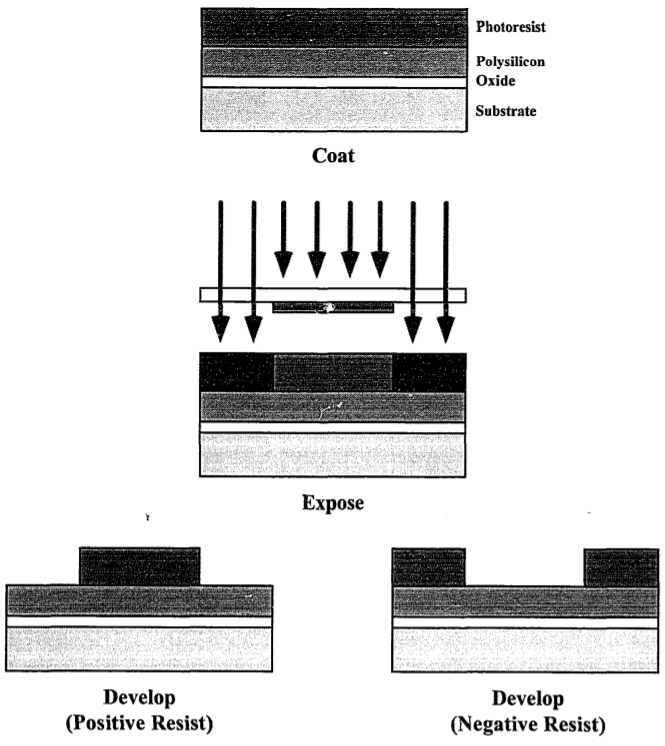
\includegraphics[scale = .75]{Figure 1.1}
	\caption{The lithographic process.}
	\label{fig:1.1}
\end{figure}

\begin{figure}[H]
	\centering
	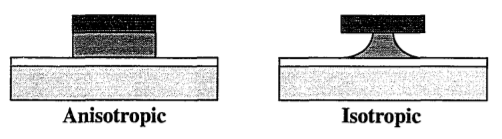
\includegraphics[scale = .75]{Figure 1.2}
	\bf\caption{Anisotropic and isotropic etching of small linewidths.}
	\label{fig:1.2}
\end{figure}

\noindent\textbf{Selectivity:} The etch rate ratio between the layer being etched and other \\
\indent layers, such as the photoresist or the underlying film.

\vspace{.25cm}

\noindent\textbf{Anisotropy:} The dependence of etch rate on direction. This usually refers to 
\indent greater
vertical than horizontal etch rate.

\vspace{.25cm}

\noindent\textbf{Uniformity:} The variation of the etch across the entire wafer or between\\ 
\indent multiple wafers in batch reactors.

\vspace{.25cm}

\noindent\textbf{Surface Damage:} Damage to the surface caused by the etch.

\vspace{.25cm}

A useful etch process has a number of requirements on these characteristics [108]. In order to achieve high throughput, the etch rate should be rapid. Additionally, in many recipes the etch time is predetermined; therefore, the etch rate needs to have little variation from run to run. In order to preserve the integrity of the masked pattern, the etch needs to be highly selective with respect to the masking layer; otherwise mask erosion will lead to changes in critical dimensions. Selectivity to the underlying layer is also necessary, as it is important not to remove a significant amount of material from this layer. This is especially important in the etching of polysilicon where the gate oxide below the polysilicon can be as thin as lOOÂor less. The etch needs to be highly uniform so that the same amount of material is removed across the entire wafer. The degree of anisotropy is important in order to achieve an acceptable sidewall profile. Sidewall profiles need to be vertical when etching 

\begin{figure}[H]
	\centering
	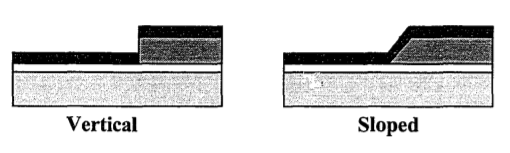
\includegraphics[scale = .75]{Figure 1.3}
	\bf\caption{Step coverage over vertical and sloped sidewalls.}
	\label{fig:1.3}
\end{figure}

\noindent small linewidths; otherwise there will be a loss in the integrity of the transfered pattern,as shown in Figure 1.2. However, as is shown in Figure 1.3, sloped sidewalls are necessary when step coverage by subsequent materials is required. Finally, the electrical properties of the material below that layer being etched must be undamaged.

One of the early techniques for removing materials is known as wet etching. In wet etching the wafers are dipped into a liquid solution, such as hydrofluoric acid (HF), which chemically reacts with the exposed surface. Through the appropriate choice of chemistry, it is possible to get very high selectivity to both the mask and underlying layer. However, wet etching is isotropic \footnote{There are situations where the orientation of the crystal can lead to an anisotropic wet etch, but these are beyond the scope of this introduction.}; i.e., material is physically removed in a direction normal to the surface. As depicted in Figure 1.2, when the critical dimensions are of the same size as the thickness of the layer being etched, isotropic etching can lead to significant changes in the desired linewidths. In this case, it is desirable to have a controlled degree of anisotropy in the etch.

As linewidths became smaller, an alternative technique known as dry etching emerged. In this technique, wafers are etched by being exposed to a low temperature plasma, as opposed to a liquid etchant. Dry etching can be broken down into a number of different regimes: plasma etching, sputter etching, and reactive ion etching. In plasma etching, neutral radicals generated in the plasma chemically react with the wafer surface to removematerial. This process tends to be highly isotropic in nature. In sputter etching (or a related technique known as ion milling \footnote{Ion milling is similar to sputter etching except that ions are not generated in a plasma but from an ion
	source in a high vacuum environment.}), material is physical removed by high energy ion bombardment [43]; this provides highly anisotropic etching but unacceptable selectivities and surface damage. In between these two extremes is reactive ion etching, where the etch is both chemical and physical in nature. By the appropriate choice of conditions, tradeoffs between anisotropy, selectivity, and surface damage can be made. Today, reactive ion etching is the main etch process used in integrated circuit production.


\section{Reactive Ion Etching}

\tab In reactive ion etching, material is removed through the interaction of neutral radicals and ions from the plasma with the wafer surface. In this section, I will first present an overview of the plasmas used for reactive ion etching. This will be followed by a discussion of the various etch mechanisms.

\subsection{Plasma Properties}

\tab A plasma is a collection of free charged particles moving in random directions; on average a plasma is electrically neutral and thus exhibits no net charge [68]. Plasmas used for semiconductor fabrication are, in general, weakly ionized, electrically driven, and not in thermal equilibrium. Overviews of plasmas used for microelectronic processing can be found in [16,45,68,108].

In reactive ion etching, the plasmas are generated in a vacuum chamber at pressures between 5 and 100 mTorr. A typical parallel plate reactive ion etcher is shown in Figure 1.4. A
mixture of gases enters the chamber through a showerhead in the upper electrode. Chamber pressure is controlled by a throttle

\begin{figure}[H]
	\centering
	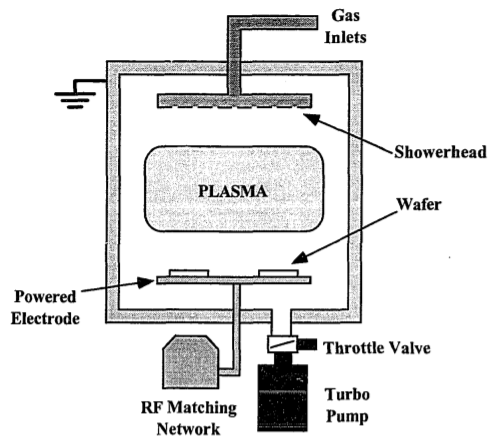
\includegraphics[scale = .75]{Figure 1.4}
	\bf\caption{Typical parallel plate reactive ion etcher}
	\label{fig:1.4}
\end{figure}

\noindent or sliding valve which regulates the exhaust of process gases by a high vacuum pump. A high frequency \footnote{Typically 13.56 MHz, a frequency which has been allotted by the Federal Communications Commission for industrial, scientific, and medical use [101].} rf generator is capacitively coupled to the lower electrode, while the showerhead and chamber walls are grounded. The application of
a large electric field across the electrodes results in ionization of the feed gas and generation of the plasma.


The electric field causes free electrons in the chamber to accelerate to high energies (~ 2eV) and these electrons collide with various species in the gas, thereby inducing a number of reactions. The most important of these collisions in sustaining the plasma is electron impact ionization in which the primary electron removes an electron from the atom, producing a positive ion and two electrons [16]. These two electrons are accelerated by the field and produce additional collisions, often causing more ionizations. It is this chain reaction that sustains the plasma. If the colliding electron does not have sufficient energy to ionize the atom, it still may excite a bound electron to a higher energy level. When this electron relaxes down to a lower energy state, the atom emits a photon. It is this process that gives a plasma its characteristic glow and why plasmas are often referred to as glow discharges. Electrons may also collide with molecules and break the bonds between atoms. This dissociation process results in atoms and molecules, both neutral and ionized. Typically, on the order of 10\% of the feed gas is dissociated [42]. Even with all of these
various collision processes, the ionization for plasmas used in RIE is typically between 10\textsuperscript{-6} and 10\textsuperscript{-4}; hence, these plasmas are made up mostly of neutral molecules.

The feed gas mixture used to produce the plasma depends on the material being etched. The chemistries used to etch various materials are shown in Table 1.1. In this research,
real-time control was applied to CF4 and CF4/O 2 etching of polysilicon. A large number of reactions occur in these plasmas; many of which are listed in [12,27]. The dominant
reactions include [91]


\begin{align}
	e^{-} + \text{CF}_{4} &\rightarrow \text{CF}^{+}_{4} + \text{F} + 2e^{-},\\
	e^{-} + \text{CF}_{4} &\rightarrow \text{CF}_{4} + 2\text{F} + 2e^{-},\\
	\text{CF}_{3} + \text{CF}_{3} &\rightarrow \text{C}_{2}\text{F}_{6},\\
	\text{CF}_{3}+\text{F} &\rightarrow \text{CF}_{4},\\
	\text{CF}_{2}+2\text{F} &\rightarrow \text{CF}_{4}.
\end{align}

The acceleration of the electrons by the rf field not only causes dissociation and ionization of the gas species, but also induces a bias on the electrode. This can be seen by assuming that the plasma potential is near zero, with respect to ground, and considering the model of

\begin{table}[H]
	\centering
	\begin{tabular}{|c|c|}
		\hline
		Material & Plasma Chemistries \\
		\hline
		Si & $\text{CF}_{4} $, $\text{CF}_{4}$/$\text{O}_{2} , \text{CI}_{2}, \text{SF}_{6}/\text{O}_{2}/\text{CI}_{2}, \text{NF}_{3}, \text{CCI}_{4}, \text{Br}_{2}$ \\
		\hline
		$\text{SiO}_{2}$ & $\text{CF}_{4}, \text{CF}_{4}/\text{H}_{2}, \text{CHF}_{3}\text{O}_{2}$ \\
		\hline
		$\text{SiN}_{3}$ & $\text{CF}_{4}/\text{O}_{2}/\text{H}_{2}, \text{CHF}_{3}$ \\
		\hline
		Silicides & $\text{O}_{2}, \text{CF}_{4}/\text{O}_{2}, \text{SF}_{6}/\text{O}_{2}$\\
		\hline
		Al & $\text{BCI}_{3}, \text{BCI}_{3}/\text{CI}_{2}, \text{CCI}_{4}/\text{CI}_{2}/\text{BCI}_{3}, \text{SiCl}_{4}/\text{Cl}_{2}$ \\
		\hline
	\end{tabular}
	\bf\caption{ Etch chemistries.}
	\label{table:1.1}
\end{table}

\noindent the rf discharge circuit shown in Figure 1.5. In this figure, $\text{V}_{a}$ is the voltage of the generator, $\text{V}_{b}$ is the voltage of the powered electrode, $\text{V}_{1}$ is the potential between the plasma and the powered electrode, $\text{V}_{2}$ is the potential between the plasma and the grounded electrode, and $\text{A}_{1}$ and $\text{A}_{2}$ are the surface areas of the powered and grounded electrodes, respectively. In order to sustain the discharge, ion current to the electrode must balance the electron current. Because the electrons are much lighter than the ions ($m_{e} \approx 10^{-4}m_{i}$), they require a much smaller field to conduct a given current. In order to balance the electron and ion fluxes, a negative dc bias develops on the powered electrode [52]. Therefore, as shown in Figure 1.6, $\text{V}_{b}$ is positive for only a small portion of the rf cycle. The thickness across which this dc voltage develops is known as the sheath. The presence of the bias voltage leads to almost continuous bombardment of the wafer by the ions. At the same time, due to their small mass, electrons are rapidly accelerated away from the electrode. Therefore, the electron density in the sheath is drastically reduced. The electrons that are present in the sheath can gain higher energy from the field than those in the bulk plasma. When these electrons collide with atoms in the sheath, they are more likely to cause ionization, rather than excitation events [108]. This leads to less photon emission from relaxation of excited

\begin{figure}[H]
	\centering
	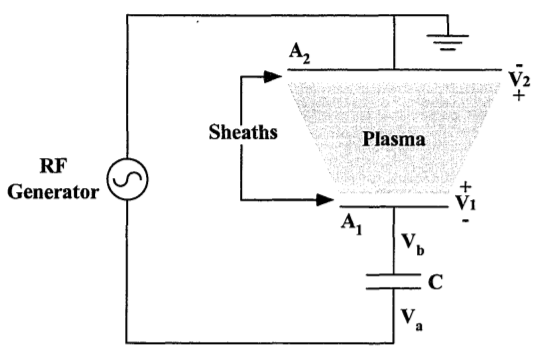
\includegraphics[scale = .75]{Figure 1.5}
	\bf\caption{Schematic of an rf discharge circuit.}
	\label{fig:1.5}
\end{figure}

\begin{figure}[H]
	\centering
	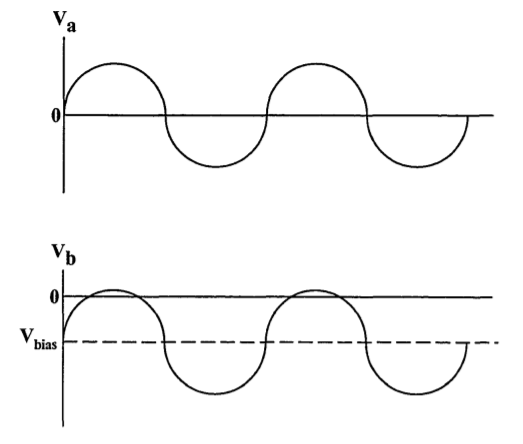
\includegraphics[scale = .75]{Figure 1.6}
	\bf\caption{Voltage waveforms in rf discharge.}
	\label{fig:1.6}
\end{figure}

\noindent atoms than in the bulk; therefore, the sheaths are darker than the rest of the discharge and are also referred to as dark spaces. Complete details of this phenomenon can be found in
[16].

A sheath also develops between the plasma and the grounded electrode leading to a positive plasma potential (V2 ). If it is assumed that the ions traverse the dark space without collision then the voltages between each electrode and the plasma are related by [63]

\begin{align}
	\left( \frac{V_{1}}{V_{2}} \right) &= \left( \frac{A_{2}}{A_{1}} \right) ^{4}
\end{align}

\noindent However, in practice most experiments have shown that

\begin{align}
	\left( \frac{V_{1}}{V_{2}} \right) &\approx \left( \frac{A_{2}}{A_{1}} \right) ^{q}
\end{align}


with q $leq$ 2.5. It is thought that this difference is because the sheaths are not completely collisionless [16]. At process conditions used in this research the mean free path of the ions was on the order of 4 mm and the sheath thickness was measured to be approximately 13 mm. Therefore, ions collide rarely while traversing the dark space and the above relationship approximately holds. In RIE, the chamber walls are part of the grounded electrode; hence, the grounded electrode generally has a much larger surface area than has the powered electrode. This leads to a large bias between the plasma and the powered electrode ($V_{1}$), and a small one with respect to ground ($V_{2}$). The resulting potential distribution is similar to that shown in Figure 1.7. In this figure, the dc bias voltagE refers to the bias of the powered electrode with respect to ground.


\subsection{Etch Mechanisms}

\tab Reactive ion etching is actually a misleading name for the process [21]. A more descriptive name would be ion enhanced etching. In the RIE process, the surface is exposed to both thermal radicals and high energy ions.

\begin{figure}[H]
	\centering
	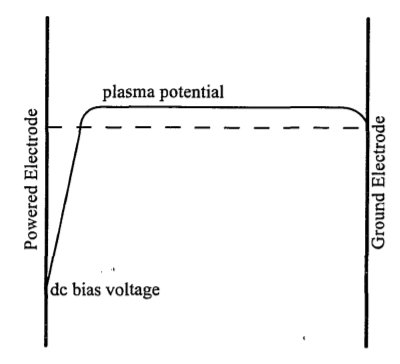
\includegraphics[scale = .6]{Figure 1.7}
	\bf\caption{Potential distribution in an asymmetric parallel plate reactor.}
	\label{fig:1.7}
\end{figure}

\noindent In the case of silicon etching performed in a tetrafluoromethane ($CF_{4}$) plasma, the neutral radicals are fluorine atoms and the ions are mainly $CF^{+}_{3}$. Reactions at the surface lead to the formation of $SiF_{4}$ which desorbs, removing silicon from the surface (Figure 1.8).

\begin{figure}[H]
	\centering
	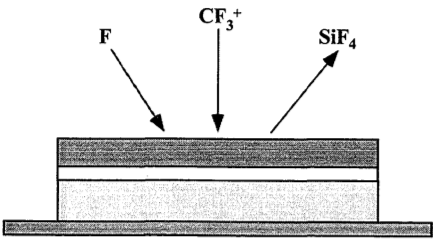
\includegraphics[scale = .6]{Figure 1.8}
	\bf\caption{Etch species and product.}
	\label{fig:1.8}
\end{figure}

\large\bf Role of neutral radicals
\vspace{.5cm}

\normalfont\normalsize A number of steps must occur for etching to take place at the wafer surface. First, the radicals must diffuse to the wafer and adsorb onto the surface. The radicals then react with the surface material to form a volatile reaction product. Etching is complete when these reaction products desorb into the gas phase and diffuse away from the wafer surface. In the case of fluorine etching of silicon, these steps are

\setstretch{1.1}
\begin{align}
	\text{Absorption: }& \text{F}_{gas} \rightarrow \text{F}_{ads}, \\
	\text{Reaction: }& \text{Si}+4\text{F}_{ads} \rightarrow \left( \text{SiF}_{4}\right)_{abs}, \\
	\text{Desorption: }& \left( \text{SiF}_{4}\right)_{abs} \rightarrow \left( \text{SiF}_{4}\right)_{gas},
\end{align}

\noindent where the subscript ÿas denotes species in the gas phase and ads denotes species adsorbed onto the silicon surface. All of these steps are necessary for etching to proceed and any of them can limit the etch rate.

The adsorption step can be rate limited by the supply of fluorine at the surface. Therefore, the flux of fluorine radicals is an important parameter in controlling the etch. In general, the flux of a neutral species is given by [16]


\setstretch{.5}
\begin{align}
	\Gamma_{x} &= \frac{n_{x}\bar{c}_{x}}{4} \text{ per unit area,}
\end{align}

\setstretch{1.5}
\noindent where $n_{x}$ is the concentration and $\bar{c}_{x}$ is the mean speed of species $x$. The mean speed is given by

\setstretch{.4}
\begin{align}
	\bar{c}_{x} &= \left( \frac{8kT}{\pi m_{x}}^{\frac{1}{2}} \right)
\end{align}

\setstretch{1.5}
\noindent where T is the temperature of species $x, m_{x}$, is the mass of species $x$, and $k$ is Boltzmann’s constant. From this equation, it can be seen that the flux of fluorine radicals is proportional to their concentration in the plasma. This fact was important to the development of the control strategy.

\setstretch{1.5}
\noindent\large\bf Role of the Ions

\normalsize\normalfont The role of the ions is not to react with the surface but to enhance reactions involving silicon and fluorine on the surface. In capacitively coupled plasmas, such as those used in reactive ion etching, the etch yield (sihcon atoms etched per incident ion) is typically around 8 [103]. The major etch product is $\text{SiF}_{4}$; therefore, the removal of 8 silicon atoms requires 32 fluorine radicals. This is much more than can be provided by a single $\text{CF}^{+}_{4}$ ion. The main effect of the ions is therefore to enhance the chemical etching process.


There have been several mechanisms proposed to explain the effect of ion bombardment [73]. These include chemically enhanced physical sputtering [75], surface damage enhanced reaction rates [35], and ion assisted gas-surface chemistry. The latter is generally accepted for the case of fluorine etching of silicon [103]. It is believed th at the energy supplied by ions impacting the surface increases the surface mobility, and thus enhances the formation and desorption of volatile products.


Ion bombardment can also change the nature of the reactions on the surface. Molecules of $\text{SiF}_{x}$ will not spontaneously react to form volatile $\text{SiF}_{4}$; thus atomic fluorine is necessary for etching to occur [106]. However, ion bombardment will indeed cause this reaction to occur. In addition, while $\text{SiF}_{2}$ is normally strongly bound to the surface, ion collisions can leave this molecule in a weakly bound state [106]. Hence, the $\text{SiF}_{2}$ can then thermally desorb after the collision.


The degree to which the ions enhance the etch rate is a function of their incident energy. The etch yield for an ion increases with both the ion energy and the flux ratio between,

\setstretch{.75}
\begin{figure}[H]
	\centering
	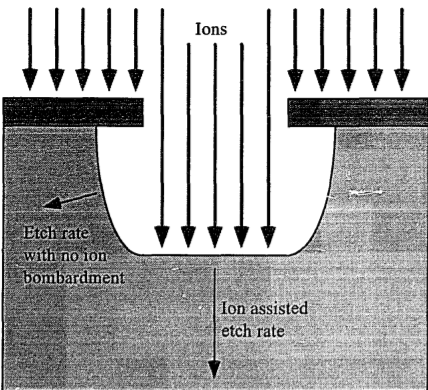
\includegraphics[scale = .5]{Figure 1.9}
	\bf\caption{Directional etch produced by ion bombardment}
	\label{fig:1.9}
\end{figure}

\setstretch{1.5}
\noindent fluorine radicals and ions, approaching saturation for high flux ratios [44]. The removal rate of silicon atoms is thus


\setstretch{.5}
\begin{align}
	\text{Etch Rate} &= p_{0} \left( \frac{\Gamma_{F}}{\Gamma_{Ions}}, \varepsilon_{Ions} \right) \text{ x } \Gamma_{Ions},
\end{align}

\setstretch{1.5}
\noindent where $p_{0}$ is the etch yield, $\Gamma_{F}$ is the flux of fluorine radicals, $\Gamma_{Ions}$ is the flux of ions, and $\varepsilon_{Ions}$ is the energy of the ions. The energy of the ions is given by

\setstretch{1}
\begin{align}
	\varepsilon_{Ions} &= q \left( V_{plasma}-V_{bias}\right),
\end{align}

\setstretch{1.5}
\noindent where $q$ is a unit charge and $V_{plasma}$ is the dc plasma potential shown in Figure 1.7. The plasma potential is generally small {$V_{plasma} \sim 20V$); therefore, assuming that most of the ions are singly charged, $qV_{bias}$ is a good estimate of energy of the ions.
	
In reactive ion etching, it is the enhancement of etch rate due to ion bombardment that causes anisotropic etching. The ions only bombard the surface in areas left unprotected by the mask. Thus, as shown in Figure 1.9, ion enhanced etching occurs on the bottom surface, of a trench, while only
	
\setstretch{1}
	\begin{figure}[H]
		\centering
		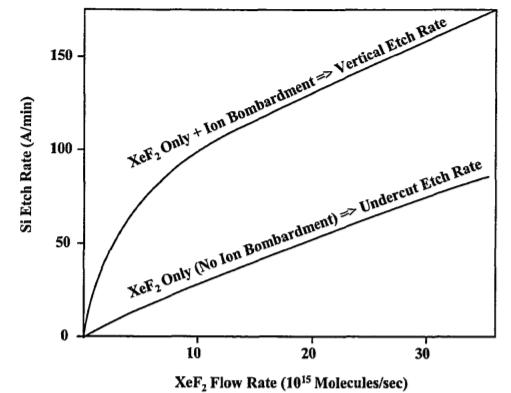
\includegraphics[scale = .6]{Figure 1.10}
		\bf\caption{ Etch rate with and without ion bombardment [38].}
		\label{fig:1.10}
	\end{figure}
	
\setstretch{1.5}
\noindent chemical etching occurs on the sidewalls. The degree of anisotropy is controlled by the flux and energy of the ions, as well as the flux of neutral radicals.
	
\setstretch{.5}
\subsection{Sidewall Passivation}
	
\setstretch{1.5}
\tab Anisotropic etching is important to the production of microelectronic devices with small linewidths. Using ion beam studies with $\text{XeF}_{2}$ gas, it has been shown (see Figure 1.10) that the vertical etch rate and undercut etch rate go to zero together [38]. Therefore, it is not possible to get vertical sidewalls with a fluorine chemistry unless some sort of sidewall passivation is used. One method of achieving vertical sidewalls is by using a chemistry that deposits a polymeric film [42]. In this case, the polymerized films deposit on all the surfaces, including the surfaces of the trench being etched. As shown in Figure 1.11, high directional bombardment by the ions removes this film from the bottom surface but leaves the walls untouched [23]. This continuous clearing of the bottom allows etching to proceed in the
	
	
\setstretch{.75}
	\begin{figure}[H]
		\centering
		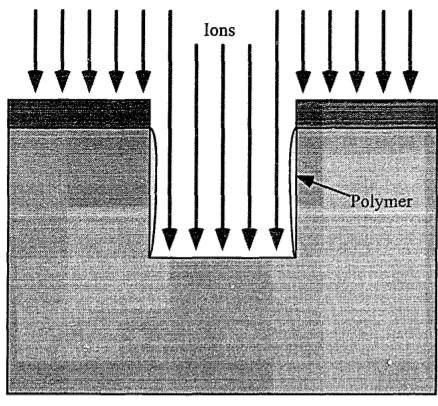
\includegraphics[scale = .6]{Figure 1.11}
		\bf\caption{ Sidewall passivation through polymerization.}
		\label{fig:1.11}
	\end{figure}
	
\setstretch{1.425}
\noindent vertical direction while the polymers inhibit etching of the sidewalls.
	
The key to this technique is to operate the plasma in a regime where polymeric films form on surfaces protected from ion bombardment while etching proceeds on the exposed surfaces. The separation between etching and polymerization can be qualitatively described by the fiuorine-to-carbon (F/C) ratio of the plasma. The ratio includes only those species which participate in the etching or polymerizing chemistry {e.g. $ \text{F}, \text{CF}_{3}, \text{CF}_{2}, \text{CF}, \text{CF}^{+}_{3} $, etc. ) and excludes inert species {e.g. $ \text{CF}_{4}, \text{C}_{2}\text{F}_{6}, \text{SiF}_{4}, \text{CO}, \text{CO}_{2}, \text{HF},$ etc. ). Increasing the ratio leads to increased Si etch rates, and decreasing the ratio lowers the etch rates and encourages polymerization [108]. The threshold between etching and polymerization varies with $\text{V}_{bias}$ as shown in Figure 1.12. The F/C ratio can be varied by the addition of $\text{O}_{2}$ or $\text{H}_{2}$ to the feed gas. The addition of $\text{O}_{2}$ to the plasma chemistry consumes C (by forming CO and $\text{CO}_{2}$), while the addition of $\text{H}_{2}$ consumes F (by forming HF). By controlling the gas chemistry, polymers can be selectively deposited on the sidewalls and thus lead to anisotropic etching.
			
\begin{figure}[H]
	\centering
	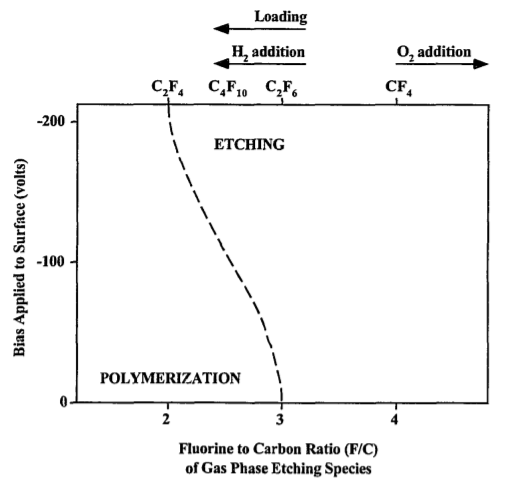
\includegraphics[scale = .6]{Figure 1.12}
	\bf\caption{ Boundary between polymerization and etching as influenced by F /C ratio [23].}
	\label{fig:1.12}
\end{figure}		
			
\section{Applications of Feedback Control to Semiconductor Fabrication Processes}
			
\setstretch{1.5}
\tab Traditional process control in the semiconductor industry has been primarily based on a collection of separate feedback loops relating one measurement of interest to one actuator. Over the past decade, there have been a number of different applications of multivariable feedback control to a variety of fabrication steps. Common to all of these applications is that the control algorithms are based on models of the particular process and in  cases multiple process parameters (either of different process variables or of a single variable at different locations) are controlled by manipulating various equipment parameters. In addition, they all use real-time feedback in the sense that equipment parameters are manipulated during the process to maintain specified process conditions.
			
			
One of the first such applications was undertaken at the University of Texas at Austin. This group explored real-time monitoring and control for reactive ion etching of silicon and silicon dioxide [13,76,77]. This work applied block relative gain array analysis to silicon and silicon dioxide etching with both $\text{CF}_{4}/\text{O}_{2}$ and $\text{CF}_{4}/\text{H}_{2}$ plasmas. It was seen that single loop feedback control was inadequate for both of these etching processes [13]. Multivariable control was found to be effective in reducing dynamic process fluctuations.
			
			
During the fall of 1991, members of the Solid-State Electronics Laboratory and the Control Systems Laboratory at the University of Michigan began joint work on controlling the reactive ion etching process for polysilicon gate etching. An overview of applications of real-time feedback control to RIE at the University of Michigan was presented at the Electrochemical Society’s 187th Meeting [46]. The basic idea of the control strategies is to decompose the reactive ion etching process into a plasma generation process and a wafer etch process. This will be discussed in detail in Section 3.1. Control of plasma characteristics has been shown to reject disturbances to the etch process [29,86,87]. The effect of controlling different sets of plasma characteristics was also explored [30], as well as the benefits of using a multiple-input multiple-output controller versus several “independent” single-input single-output controllers [30,37]. In addition, this control strategy has been applied to etching amorphous silicon for thin film transistors [51]. A similar strategy has been applied to control sidewall profile [85]. The above work has been based on linear models and controllers for the plasma generation process. Nonlinear modeling and control have also been applied [105].
			
Mutsukura, \textit{et. al}. [81] at Tokyo Denki University have applied real-time feedback to control optical sheath thickness and maximum optical intensity in etching plasmas. In this work, the spatial distribution of the optical emission intensity was measured with a CCD camera. Unlike the University of Michigan, no steps were taken to measure any particular wavelength of the emission. Prom this measurement, a sheath thickness and maximum optical intensity were extracted. A real-time feedback controller was used to regulate these plasma parameters by varying chamber pressure and applied power. It was shown that using this technique reduced the variance of etch depth over a number of trials.
			
Another application of modern control techniques has been to Rapid Thermal Processing (RTF) of single wafers. RTF is being explored as a possible way to overcome the uniformity problems associated with multiwafer furnaces [28]. A number of groups have been applying various modeling and control strategies to RTF. A joint group from Stanford University and Texas Instruments’ Microelectronics Manufacturing Science and Technology project have been using low-order nonlinear models of a RTF system [93]. This model was then linearized and its unknown parameters were fit from experimental data [19,95]. Based on this model, feedback control was applied using the Internal Model Control strategy [94]. Likewise, a group from the University of Texas at Austin [28,100] has applied a successively linearized quadratic dynamic matrix control (QDMC) strategy [11] to an RTF developed at Sematech.
			
A strategy similar to that employed at the University of Michigan is being applied to plasma enhanced chemical vapor deposition (FECVD) at Carnegie Mellon University [18,62]. This work has focused on the deposition of silicon nitride using SiIÎ4 and NH3. A quadrapole mass spectrometer is used to measure key partial pressures in the plasma.Experimental results will be presented in the near future [18].
			
All of the applications presented above focus on the processing of silicon wafers. Additionally, real-time control techniques have been applied to the processing of compound semiconductors. Looze, \textit{et al}. [71,72] have applied lead compensation to Czochralski growth of GaAs. Celii, \textit{et al}. [14] have used spectroscopic ellipsometry to control layer thicknesses in AlAs/$\text{In}_{0.53}\text{Ga}_{0.47}$As resonant-tunneling diodes grown using molecular beam epitaxy (MBE).
			
			
\section{Outline of the Dissertation}
			
\tab At the beginning of this introduction, the specific goals of this research were listed. First, it was important to configure our reactive ion etcher to allow the implementation of real-time feedback control. This will be described in Chapter 2. Next, as described in Chapter 3, a control-oriented model of the plasma generation process was developed. This model was used in Chapter 4 to design and implement a controller which rejects etch rate disturbances. The same strategy was employed in Chapter 5 to control sidewall profile. The dissertation will conclude with a discussion of future directions for this research.
			


	
	\setstretch{1.5}
\chapter{Experimental Apparatus}

\tab A major portion of the research presented in this dissertation has been experimental in nature. All of the plasma and etch experiments were performed using an Applied Materials Precision Etch 8300 (AME-8300)\footnote{The system was not truly an 8300 series etcher, but instead a hybrid between the 8100 and 8300 series. It is affectionately referred to as the “Mule.”} which was donated by the manufacturer to the SolidState Electronics Laboratory (SSEL) at the University of Michigan in 1987. This etcher, as with most commercially available etch systems, was designed for a production environment and was not configured for in situ measurements or the application of real-time control techniques. The first portion of my research focused on modifying our AME-8300 for the implementation of real-time feedback control.

\setstretch{.75}
\section{Precision Etch 8300 Hexode RIE}

\setstretch{1.5}
\tab The AME-8300 is a hexode reactive ion etcher (see Figure 2.1), where wafers are placed vertically on a hexagonally shaped powered electrode and the bell jar acts as the grounded electrode. The AME-8300 at the University of Michigan was designed to simultaneously etch 18 four inch wafers, though in this research it was used as a single wafer etcher. The hexode


\setstretch{.75}
\begin{figure}[H]
	\centering
	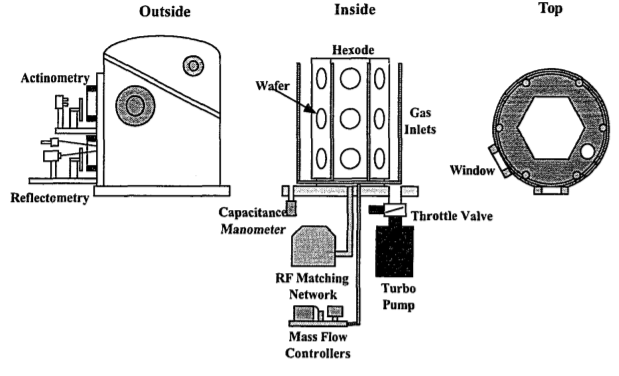
\includegraphics[scale = .6]{Figure 2.1}
	\bf\caption{ Precision Etch 8300 hexode reactive ion etcher.}
	\label{fig:2.1}
\end{figure}

\setstretch{1.5}
\noindent has approximately one third the surface area of the bell jar. As was seen in Equation 1.7, this difference in surface area allows high energy ion bombardment of the powered electrode while minimizing the bombardment of the grounded electrode and other chamber surfaces. Process gases are mixed in a manifold and then enter the chamber in a sprinkler fashion through vertical pipes across from each corner of the hexode. The gas reactants are
removed from the chamber by a turbomolecular pump with the exhaust conductance from the chamber regulated by a throttle valve. It is important to note that our system does not
have a load lock, thus requiring the chamber to be vented to atmosphere each time a wafer is loaded. As will be explained in Section 4.2.1, this has had a strong impact on the etching
process.

The AME-8300 comes standard with two viewports at which optical sensors can be mounted. One of the viewports is on the upper portion of the clam shell and moves with the top of the chamber when wafers are loaded. The other port has occasionally beenoccupied by an infrared camera and more recently by a mass spectrometer. Neither port provided a stable mounting point for the optical sensors used in this research. Therefore, two additional 4 inch optical viewports were added to the face of the reactor where the gate valve for a load lock would have been situated. Optical breadboards were mounted below each of these windows to create a flexible and sturdy platform for the optical sensors.


\subsection{Actuators}

\tab It was necessary to upgrade some of the actuators on the reactive ion etcher in order
to improve our ability to control the process. The existing throttle valve, which regulates
the exhaust of reactant gases from the chamber, had several shortcomings from the point
of view of dynamic control. These included a large leakage conductance when fully closed,
an operating regime near saturation, hysteresis in the motion of the valve, and the lack of
a sensor for measuring actual valve position. The valve was replaced with an MKS Type
652A Throttle Valve and an MKS Type 653 Throttle Valve Controller. This valve was sized
to be smaller than the old one, thus moving the operating region away from saturation. In
addition, the valve has a low leakage conductance when fully closed, a good response time,
and a sensor to measure the actual valve position. The throttle valve controller allows
either the specification of a pressure setpoint to be regulated by an internal PID loop or
the direct control of throttle position. The RF power actuator includes a Henry Electronics
2000W, 13.56 MHz generation unit and an RF Services RF8300RL matching network. The
AME-8300 was originally supplied with a Micro-Match 8300N matching network supplied by
Applied Materials. The upgraded matching network does a better job matching impedances
(as measured by reflected power), has a quicker response time, and has a peak-to-peak
voltage ($\text{V}_{pp}$) measurement. The $\text{V}_{pp}$ is used by related research efforts, but not utilized in this work. Gas flows are regulated by MKS Type 2259C Mass Flow Controllers and are mixed in a manifold prior to entering the process chamber. These flow controllers were sized to give the highest resolution over the flow rates necessary for this work.

During this research, short intermittent fluctuations in the gas flow rates were noted.
It was suspected that these were due to the pressure regulator on the gas bottles [36].
These fluctuations, while short enough to have negligible effect on etch results, could make
dynamic modeling difficult. The fluctuation problem was solved by placing a 2 $\mu m$ VCR
filter gasket in the outlet valve just downstream of the pressure regulator.

\subsection{Sensors}

\tab Three types of sensors were used to make in situ measurements of the plasma environment for feedback control. The dc bias voltage ($\text{V}_{bias}$) was measured through an inductive
tap on the powered electrode side of the matching network. Pressure in the chamber was
monitored by an MKS Type 127A Baratron Capacitance Manometer. A typical operating
regime for reactive ion etching in the AME-8300 is around 20 mTorr. The manometer, which
originally had full scale range of 1 Torr, was resized to 100 mTorr to improve its resolution.
The fluorine concentration is estimated via optical emission spectroscopy using actinometry; details of actinometry are presented in Section 2.1.3. In addition to these sensors, the
AME-8300 was fitted with a laser reflectometry system to measure in \textit{situ} etch rate; details on the reflectometry system are presented in Section 2.1.4. This measurement was only
used to verify the performance of the control schemes and not for real-time feedback.

\subsection{Fluorin Concentration Estimate}

\tab The fluorine concentration in the bulk plasma is strongly related to properties of the
etch [44]. Unfortunately, it is not possible to directly measure fluorine concentration without
perturbing the plasma. In research, various probes are sometimes used to sample the plasma
chemistry; it is very difficult to relate plasma characteristics near the probe to those of the
unperturbed plasma [56]. These probes are therefore not useful in measuring properties of
a plasma during processing. Instead, the fluorine concentration is indirectly measured via
optical emission spectroscopy using a technique known as actinometry.

\setstretch{1.75}
\noindent\large\bf Actinometry

\normalsize\normalfont The emission intensity from a spectral line of species x is given by [58]

\setstretch{1}
\begin{align}
	I_{x} &= N_{x} \left[ \int_{0}^{\infty} Q_{x}\left( P,N_e \right) \sigma_{x} \left( \epsilon \right) N_{e} d\epsilon   \right],
\end{align}



\setstretch{1.5}

\noindent where $N_{x}$ is the concentration of species $x$, $Q_{x}$ is the quantum yield from a given higher energy excited state to a given lower energy excited state, P is pressure, $\sigma_{x}$ is the excitation cross section from the ground state to a given excited state of electron energy $\epsilon$, and $N_{e}$ is the electron density in an electron energy range $d_{\epsilon}$. Because several of these parameters are unknown and impossible to measure, we use a technique known as actinometry [22]. In actinometry, a small amount of an inert gas, having excitation characteristics similar to the species of interest, is added to the feed gas; the inert gas is referred to as an actinometer. As will be seen below, the appropriate choice of spectral lines allows the concentration $N_{x}$ to be determined without calculating the integral in Equation 2.1. Argon is used as an actinometer for fluorine concentration estimates.

The fluorine concentration estimate is found by first noting that the spectral line intensities are proportional to the corresponding excited state population densities ($N_{x}^{*}$) of each of the species,

\setstretch{1}
\begin{align}
	I_{F} \alpha N_{F}^{*}
\end{align}

\noindent and

\begin{align}
	I_{Ar} \alpha N_{Ar}^{*}.
\end{align}

\setstretch{1.5}

\noindent It is necessary that the excitation efficiencies for the excited states corresponding to the spectral lines used in actinometry have similar dependence on plasma parameters [22]. In practice, both excited states need to have similar excitation thresholds and must only be populated from the ground state by electron collisions.

For fluorine actinometry, the 703.75 nm and 750.39 nm emission lines of fluorine and
argon, respectively, satisfy these requirements. The excited states for these transitions have
similar excitation thresholds [99], as shown in Figure 2.2. For low density plasmas, such
as those used in RIE, these states are also only populated by electron excitation from the
ground state [40]. From this choice of spectral lines:


\setstretch{0.75}
\begin{align}
	\frac{N_{F}^{*}}{N_{F}} = \frac{N_{Ar}^{*}}{N_{Ar}}.
\end{align}

\noindent Therefore, 

\begin{align}
	N_{F} = k\frac{I_{F}}{I_{Ar}}N_{Ar},
\end{align}

\setstretch{1.5}

\noindent where k is a proportionality constant known as the actinometric constant. We define $\gamma$ to be the fraction of Ar in the chamber,

\setstretch{.75}
\begin{align}
	\gamma = \frac{P_{Ar}}{P} = \frac{N_{Ar}}{N},
\end{align}

\setstretch{1.5}
\noindent where $N$ is the total concentration of species in the chamber. Note that from the ideal gas law


\setstretch{1}

\begin{align}
	N = \frac{n}{V} = \frac{P}{RT},
\end{align}

\setstretch{1.5}
\begin{figure}[H]
	\centering
	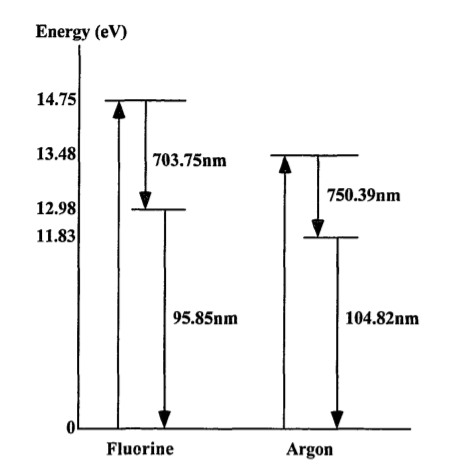
\includegraphics[scale = 1]{Figure 2.2}
	\bf\caption{ Atomic energy levels and emission wavelengths for F and Ar atoms [99].}
	\label{fig:2.2}
\end{figure}

\noindent where n is number of molecules, $V$ is the chamber volume, $P$ is the chamber pressure, $R$ is the universal gas constant ($R = 8.314 \text{J/mol } ^{\circ} K$) and T is the temperature in degrees Kelvin. Therefore,

\setstretch{1}
\begin{align}
	N_{Ar} = \gamma \frac{P}{RT}
\end{align}

\noindent and

\begin{align}
	N_{F} = k\frac{I_{F}}{I_{Ar}}\gamma \frac{P}{RT}.
\end{align}

\setstretch{1.5}

\noindent Implicit in these equations is the assumption that the neutral temperature in the plasma remains constant. This assumption is based on the fact that the radicals remain “cold” in the plasma.

In general, it is assumed that the fraction of argon in the plasma is equal to the percentage of argon in the feed gas. This assumption is reasonable as the dissociation of the feed
gases is usually between 0.01 and 10 percent [68]. This leads to the traditional estimate of
fluorine concentration

\setstretch{1}
\begin{align}
	N_{F} = \bar{k} \frac{I_{F}}{I_{Ar}}\gamma_{flw} P,
\end{align}

\setstretch{1.5}
\noindent where $\bar{k} =\frac{k}{RT}$ and $\gamma_{flw}$ is the percentage of total flow which is argon $\left( \gamma_{flw} = \frac{FLOW_{Ar}}{FLOW_{Total}} \right)$. Thus, $\gamma_{flw}$ $P$ is an estimate of the argon partial pressure ($P_{Ar}$). This equation is different from those traditionally seen in the literature [88] as it accounts for variations in the percentage of argon in the feed gas.

Throughout this dissertation no attempt was made to determine the actinometry constant $k$. In addition, during the etch rate control portion of this research the percentage of
argon in the feed gas was held constant at 5\% by premixing it with $\text{CF}_{4}$ in the gas bottle. Thus, the fluorine concentration estimate used in Chapters 3 and 4 was

\setstretch{1}

\begin{align}
	[F]= \frac{I_{F}}{I_{Ar}}P.
\end{align}

\setstretch{1.5}

In the sidewall profile control experiments, $\text{O}_{2}$ was added to the $\text{CF}_{4}$ chemistry. Initially, to insure a constant percentage of argon in the feed gas, a separate mass flow controller was used to regulate argon flow. The argon flow rate was typically quite small (~ 1.5 seem) and the exact flow rate was not very reproducible. Therefore, the premixed $\text{CF}_{4}$ /Ar bottle was again used and the percentage of argon in the gas mixture dynamically calculated. Due to this, the fluorine concentration estimate used in Chapter 5 was


\setstretch{1}

\begin{align}
	[F]= \frac{I_{F}}{I_{Ar}}\gamma_{flw}P.
\end{align}

\setstretch{1.5}

The fluorine estimator presented in Equation 2.10 assumes that the relative concentration of argon in the chamber is equal to the percentage of argon in the feed gas. In the case
when the dissociation is not negligible Equation 2.10 overestimates the actual fluorine concentration. In addition, as shown in Figure 2.3, outgassing from the chamber walls serves
to dilute the argon partial pressure. This is particularly a problem for the reactor used in
this research, as it does not have a load lock. It was necessary to expose the chamber to
the ambient atmosphere every time a wafer was loaded to be etched. In doing this, water
vapor adsorbs on the walls of the chamber; this moisture then desorbs when the plasma is
struck. Because of the large surface area of the chamber walls, the moisture causes a large
disturbance to the plasma which decays with a time constant on the order of 300 seconds.
The effect of this disturbance on the etching process will be discussed in Section 4.2.

One solution to the problems associated with dilution of the actinometer is to measure
the actual argon partial pressure in the chamber. This has been done by Jenq, \textit{et al.} ,
for both RIE and electron cyclotron resonance (ECR) plasma using a mass spectrometer
[58]. They noted that ion concentration was independent of applied power in RIE; this was
not the case for ECR plasmas. This fact supports the assumption that there is a small
percentage of dissociation in the plasma. Though not used in this research, an Extrel MS


\setstretch{1}
\begin{figure}[H]
	\centering
	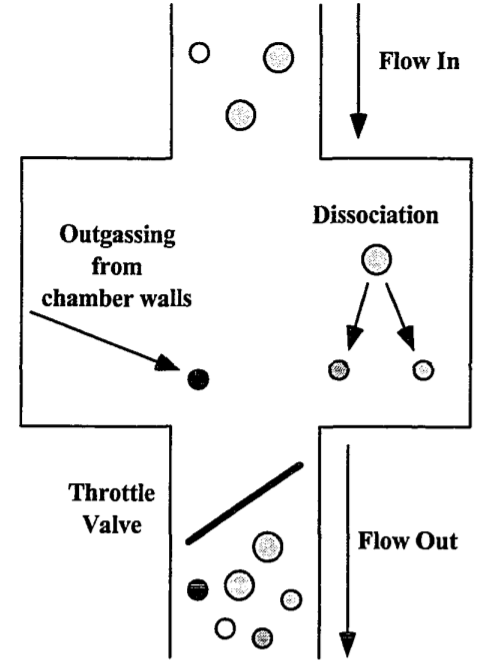
\includegraphics[scale = .5]{Figure 2.3}
	\bf\caption{ Dilution of actinometer.}
	\label{fig:2.3}
\end{figure}

\setstretch{1.5}

\noindent 250 mass spectrometer has recently been added to our AME-8300. It is our hope that this will allow us to account for argon dilution caused by outgassing from the chamber walls.


\setstretch{1.75}
\noindent\large\bf Optical Emission Hardware

\normalsize\normalfont The optics for collecting plasma emissions have gone through several iterations over the time period of this work, with the goal of providing better day-to-day repeatability and accuracy of the optical measurements. In the discussion below, I will only present the current system configuration.

The actinometry system is shown in Figure 2.4. Optical emission from the plasma is
modulated to 1 kHz using a mechanical chopper and is collected by a fused silica fiber
bundle. This bundle is bifurcated and sent to two Spex 500M 1 /2 meter monochromators,
each with a 1200 grooves/mm holographic grating with blaze wavelength of 750 nm. The


\setstretch{1}
\begin{figure}[H]
	\centering
	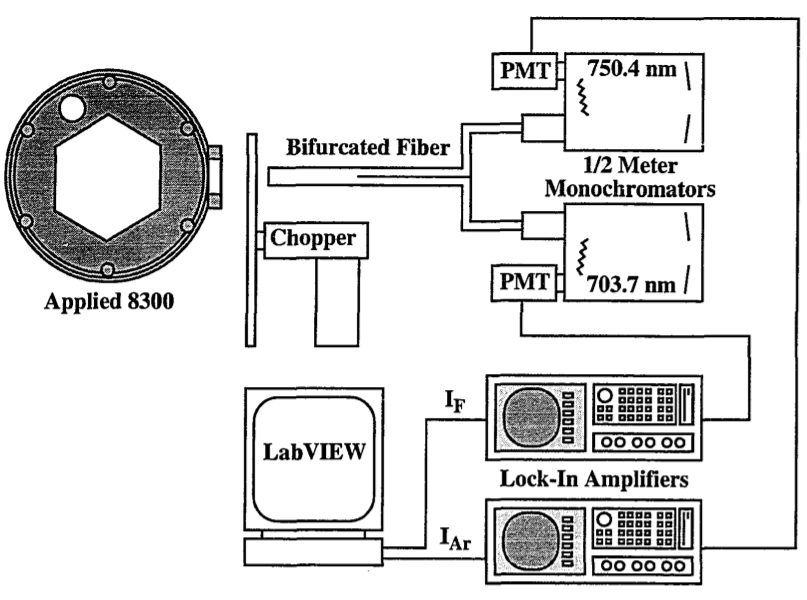
\includegraphics[scale = .5]{Figure 2.4}
	\bf\caption{ Actinometry system.}
	\label{fig:2.4}
\end{figure}

\setstretch{1.5}

\noindent monochromators are calibrated using micro-stepper motors to the 703.7 nm and 750.4 nm
wavelengths of the fluorine and argon spectra, respectively. The light is converted into
electrical signals using thermoelectrically cooled Hamamatsu R928 photomultiplier tubes
and demodulated with Stanford Research SR850 DSP Lock-In Amplifiers with a low pass
filter time constant of 30 ms. These amplifiers use automatic phase correction, thus reducing
sensitivity to chopper variations due to rf interference [9]. This system can also be used in
a scanning mode to find the optical spectrum of the plasma. Figure 2.5 shows the optical
spectrum between 675 and 775 nm for a $\text{CF}_{4}$/Ar plasma.

\setstretch{1}
\begin{figure}[H]
	\centering
	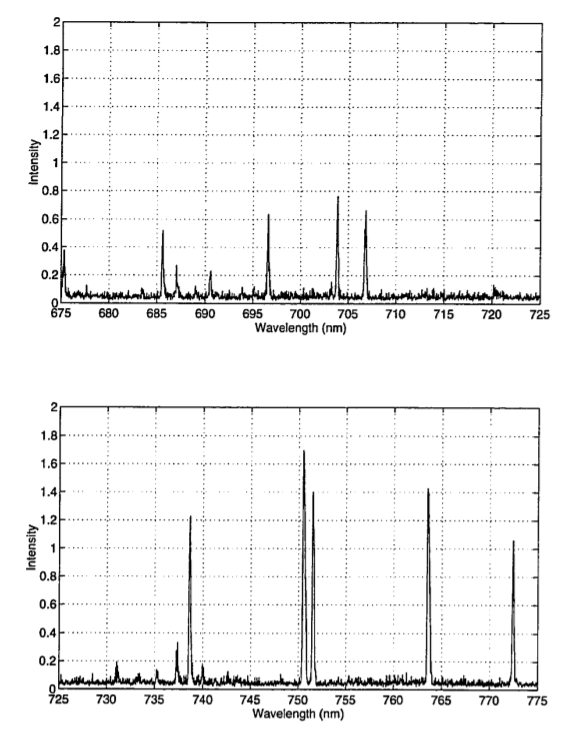
\includegraphics[scale = .8]{Figure 2.5}
	\bf\caption{ Optical spectrum of a $\text{CF}_{4}$ / Ar plasma.}
	\label{fig:2.5}
\end{figure}

\setstretch{1.5}

\subsection{Etch Rate Measurement}

\tab One of the performance metrics used for evaluating the effectiveness of the control
strategies was their the ability to reject disturbances to etch rate. In order to make this
evaluation, the etch rate was measured during the length of the run through optical interferometry. After presenting a brief overview of interference from thin films, the hardware
used in this research will be presented.

\setstretch{1.5}
\noindent\large\bf Interference in thin films

\setstretch{1.5}

\normalsize\normalfont Due to optical interference, a stack of thin film layers exhibits a reflectance that is dependent on the wavelength of the incident light and the thicknesses of each film layer. This is seen by first noting that the change in phase of light traversing the $m$th layer of film is given by


\setstretch{.5}
\begin{align}
	\delta_{m} = \frac{2\pi}{\lambda_{0}}n_{m}d_{m}\text{cos}\psi_{m},
\end{align}

\setstretch{1.5}

\noindent where $\lambda_{0}$ is the wavelength of the light in a vacuum, is the index of refraction of layer $m$, $d_{m}$ is the thickness of layer $m$, and $\psi_{m}$ is the angle at which the light is incident on the interface between layers $m$ — 1 and $m$. For light at normal incidence, the Fresnel reflection and transmission coefficients for an interface between films $m$ - 1 and $m$ are given by [49]


\setstretch{.4}

\begin{align}
	r_{m} = \frac{n_{m-1}-n_{m}}{n_{m-1}+n_{m}}
\end{align}

\noindent and

\begin{align}
	t_{m} = \frac{2n_{m-1}}{n_{m-1}+n_{m}},
\end{align}

\setstretch{1.5}
\noindent respectively. For light at angles other than $\psi_{m}=0$ see [50].

We consider the stack of $k$ thin film layers on a thick substrate (as shown in Figure 2 .6 )
and adopt the convention that $E_{m}^{+}$ is the electric field traveling down at interface $m$ and $E_{m}^{-}$ 


\begin{figure}[H]
	\centering
	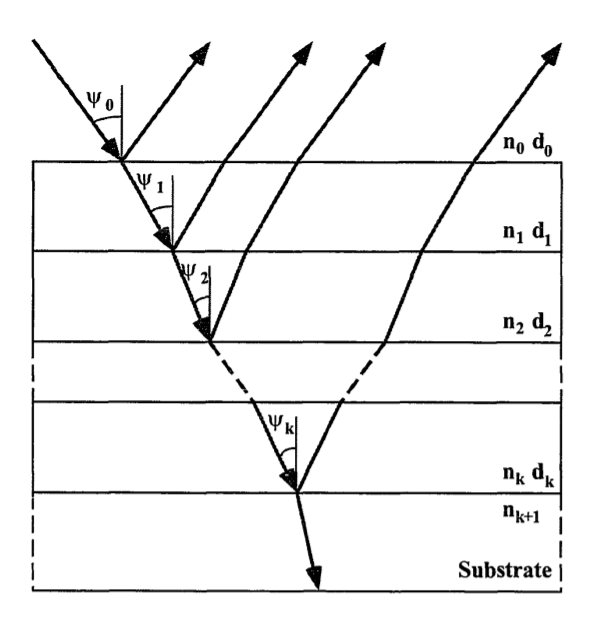
\includegraphics[scale = .8]{Figure 2.6}
	\bf\caption{ Stack of thin film materials.}
	\label{fig:2.6}
\end{figure}

\noindent likewise refers to the electric field traveling up. A similar convention is also adopted for the magnetic field $H$. The following relationship is obtained by solving Maxwell’s equations at each interface [49]


\setstretch{1}
\begin{align}
	\begin{bmatrix} E_{0}^{+} \\ E_{0}^{-} \end{bmatrix} = \frac{(C_{1})(C_{2})...(C_{k+1})}{t_{1}t_{2}...t_{k+1}} \begin{bmatrix} E_{k+1}^{+} \\ E_{k+1}^{-} \end{bmatrix},
\end{align}

\noindent where

\begin{align}
	(C_{m}) = \begin{bmatrix} e^{j\delta_{m-1}} & r_{m}e^{j\delta_{m-1}} \\ r_{m}e^{-j\delta_{m-1}} & e^{-j\delta_{m-1}} \end{bmatrix}.
\end{align}

\noindent We write the matrix product as

\begin{align}
	(C_{1})(C_{2})...(C_{k+1})=\begin{bmatrix} a & b \\ c & d \end{bmatrix}.
\end{align}

\setstretch{1.5}

\noindent If the substrate is thick compared to the absorption wavelength of the incident light, then there is no negative traveling wave at the last interface, i.e., $E_{k+1}^{-} = 0$; thus from Equation 2.16 we obtain


\setstretch{1.5}
\begin{align}
	\frac{E_{0}^{-}}{E_{0}^{+}} = \frac{c}{a}.
\end{align}

\noindent The reflectance $R$ of the multilayer stack is therefore given by [49]

\begin{align}
	R=\frac{\left( E_{0}^{-}\right)\left(E_{0}^{-}\right)^{*}}{\left(E_{0}^{+}\right)\left(E_{0}^{+}\right)^{*}} = \frac{cc^{*}}{aa^{*}}
\end{align}

\setstretch{1.5}
The interference between light reflected from the various surfaces changes as material is removed during the etching process. Therefore, a measurement of the reflectance of the
wafer can be used to determine etch rates during an etch.


\setstretch{1.5}
\noindent\large\bf Reflectometry Hardware

\setstretch{1.5}

\normalsize\normalfont The reflectometry system shown in Figure 2.7 is based on a single wavelength source, provided by a HeNe laser. The beam is modulated by a mechanical chopper before entering

\setstretch{1}
\begin{figure}[H]
	\centering
	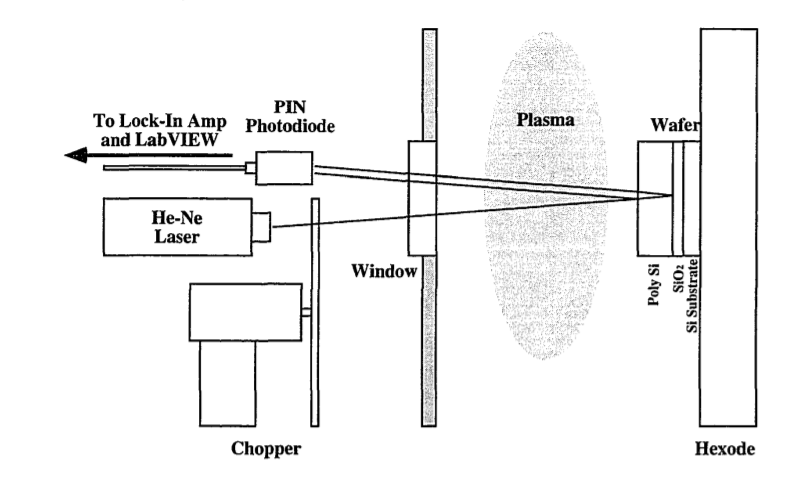
\includegraphics[scale = .7]{Figure 2.7}
	\bf\caption{ Reflectometry system .}
	\label{fig:2.7}
\end{figure}

\setstretch{1.5}

\noindent the chamber. The reflected beam is then collected by a Thorlabs PDA50 p-i-n photodiode and amplified by a Stanford Research SR530 Lock-In Amplifier with a low pass filter time constant of 1 second. This amplifier does not have an automatic phase correction feature,
but this was not a problem as there is ample signal-to-noise in this signal.

A typical trace of the reflectometry signal is shown in Figure 2.8. It can be found
from Equation 2.20 that for a single wavelength of light at normal incidence ($\Psi_{0} = 0$), the peaks and valleys in the interference pattern correspond to thickness differences of
$\frac{1}{4}\frac{\lambda_{0}}{\operatorname{Re}(n)}$ where $\operatorname{Re}(n)$ is the real component of the index of refraction of the layer being etched. For the HeNe wavelength of 632.5 nm, the time between a peak and valley corresponds to the etching of 417$\mathring{A}$ of polysilicon ($\operatorname{Re}(n) = 3.768$). The x’s in Figure 2.9 show the average etch rate (417$\mathring{A}$ divided by the time between the peak and valley) plotted at the midpoint of

\setstretch{1}
\begin{figure}[H]
	\centering
	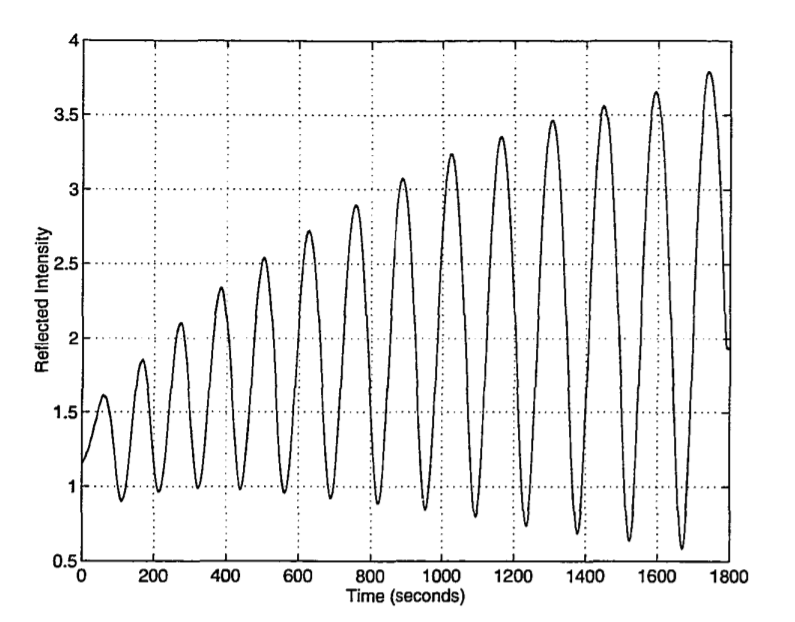
\includegraphics[scale = .55]{Figure 2.8}
	\bf\caption{ Sample reflectometry signal.}
	\label{fig:2.8}
\end{figure}

\setstretch{1.5}
\noindent each time interval. From this figure there appears to be an oscillation in the etch rate, but
this actually is due to the fact that the surface roughness of the polysilicon layer was not
accounted for. To help in visualizing the actual etch rate, a smooth polynomial is fit to this
data as shown in Figure 2.9. Note that data points are only available approximately once
a minute. This is too slow to be used for real-time feedback.

Though not used in this research, two efforts have recently been undertaken to provide
an etch rate measurement for real-time feedback. One of these involves developing an etch
rate estimator which can extract information out of the HeNe signal at a much higher
frequency [104]. The other utilizes a broader band light source, provided by a tungsten
halogen lamp, and a CCD array as a detector [9].


\setstretch{1}
\begin{figure}[H]
	\centering
	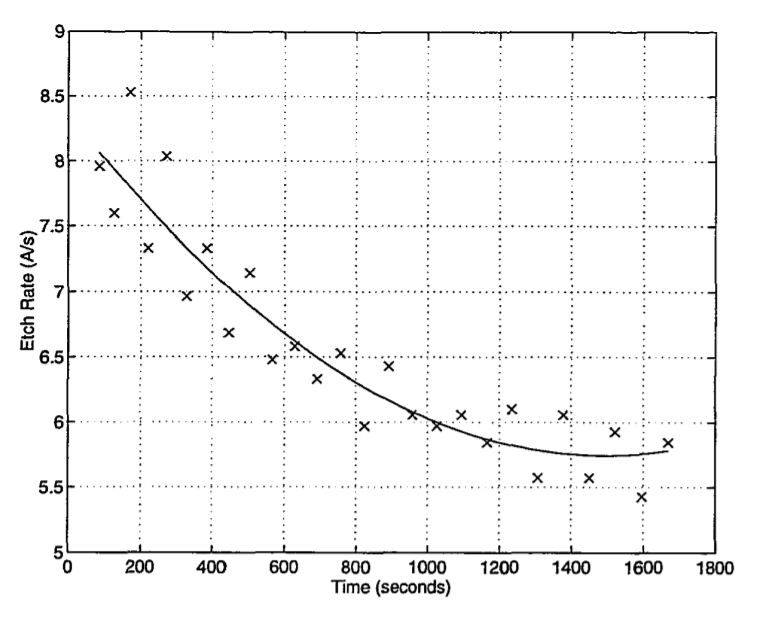
\includegraphics[scale = .55]{Figure 2.9}
	\bf\caption{  Calculated etch rates.}
	\label{fig:2.9}
\end{figure}

\setstretch{1.5}

\section{Data Acquisition and Control Platform}

\tab The largest modification made to the etcher was to upgrade its data acquisition and control software/hardware. Prior to the beginning of this work, the original control system on our AME-8300 had been replaced by a Techware Systems PAL 68000 process control computer. This system was excellent for running event-driven process recipes but was not capable of real-time monitoring and control\footnote{Recently, in joint work with Techware Systems, we have shown that it is possible to implement real-time control algorithms on Techware’s next generation of process control computers, the T-II. Work is continuing to develop a commercially available implementation.}. Two major limitations were: 1) data collection was (asynchronously) polled and 2 ) sampling rates were limited to approximately twice a second. These limitations were overcome by implementing a data acquisition and control system using LabVIEW\footnote{Lab VIEW is a graphics-based programming language from National Instruments that provide drivers for their Interface boards.
} to collect data and perform real-time control actions.


\setstretch{1}
\begin{figure}[H]
	\centering
	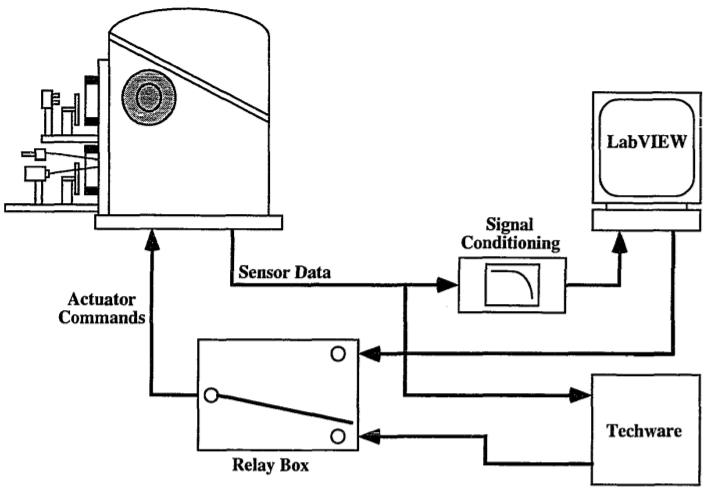
\includegraphics[scale = .55]{Figure 2.10}
	\bf\caption{  Techware and LabVIEW wiring configuration.}
	\label{fig:2.10}
\end{figure}

\setstretch{1.5}

\subsection{LabVIEW Data Acquisition and Control System}

\tab In order to provide the data acquisition and control capabilities necessary to build dynamic models and apply feedback control, an Apple Quadra 950 running LabVIEW was piggy-backed onto the Techware computer. The LabVIEW system was only used during the segment of the etch process when the plasma was lit; wafer loading, pumpdown, venting, etc. are all controlled by the Techware computer. During the time when the plasma is lit, a bank of relays gives control of the equipment setpoints to the LabVIEW system, while sensor data can be simultaneously monitored by both computers. This wiring configuration is shown in Figure 2 .10.


Our LabVIEW system consists of three expansion bus boards:

\noindent\textbf{NB-MIO-16-25L} a multifunction input-output board which has 16 signal-ended 

analog inputs, 2 analog outputs, 8 TTL inputs/outputs, and 3 counter-timers.


\noindent\textbf{NB-AO-6} an analog output board with 6 channels.


\noindent\textbf{NB-DMA-2800} which provided direct memory access (DMA) and a high speed IEEE

488 (GPIB) interface.


In developing the LabVIEW data acquisition and control system, care was taken to synchronize the timing of the various input and output channels. One of the counter/timers (CNTR\#1) was configured to produce a square wave with the period of the sampling interval. This signal is shared among the various boards via a real-time system integration (RTSI) bus, which is a local bus connecting the boards. As seen in Figure 2.11, the sample interval begins on the rising edge of the CNTR\#1 signal. When this rising edge occurs the analog output (AO) channels are updated and reading of the analog input channels (Al) is initiated. While the NB-MIO-16-25L board has 16 input channels, it only has one analog-to-digital (A/D) converter. A multiplexer switches between channels on the rising edge of an AI conversion pulse generated by a second counter (CNTR\#2). The A/D converter on this board has a settling time of 25 $\mu$s; however due to a software bug in the data acquisition drivers the period of the AI conversion pulses was set to 90 $\mu$s. The number of conversions is controlled by CNTR\#1 (the gating pulse), in that the CNTR\#2 only runs when the gating pulse is high. After all of the channels are acquired, the next control action is calculated and the inactive output buffer is loaded with the new values. More details on timing for real-time control implementations can be found in [7].


LabVIEW is a graphics-based programming language in which programs are written by “wiring” icons together. An example of LabVIEW code for reading data from the analog

\setstretch{1}
\begin{figure}[H]
	\centering
	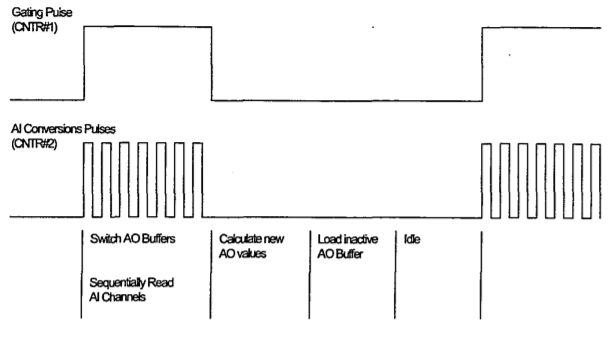
\includegraphics[scale = .65]{Figure 2.11}
	\bf\caption{  Data acquisition timing diagram.}
	\label{fig:2.11}
\end{figure}

\setstretch{1.5}

\noindent input channels is shown in Figure 2.12. LabVIEW also provides the programmer with a number of widgets in which a graphical interface (or panel) can be developed for the user. One such panel is the Control Setup Panel, shown in Figure 2.13. Prom this panel the user can select data acquisition and control parameters for the etch. It allows the user to select the controller file, reference command file and sampling rate to be used for the etch. In addition, the user can select which sensor channels will be displayed to the screen and logged to disk for future analysis. The selected sensor channels are displayed on strip charts on the Monitor Panel (Figure 2.14) during the etch.


\setstretch{1}
\subsection{Signal Preconditioning}
\setstretch{1.5}

In sampling an analog line, it is important to take precautions against a phenomenon known as aliasing [78]. If the signal being sampled contains frequency components that are higher than half the sampling frequency ($f_{s}$) then these components may appear to be low frequency components. This can particularly be a problem if there are high frequency periodic signals [6]. To prevent aliasing, a low-pass filter known as an antialiasing filter is

\setstretch{1}
\begin{figure}[H]
	\centering
	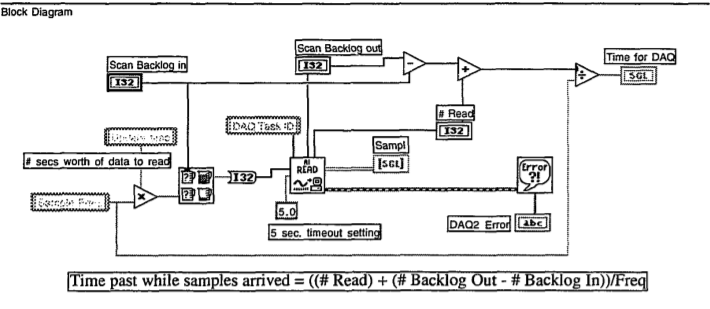
\includegraphics[scale = .7]{Figure 2.12}
	\bf\caption{  Example of LabVIEW code for data acquisition.}
	\label{fig:2.12}
\end{figure}

\setstretch{1}
\begin{figure}[H]
	\centering
	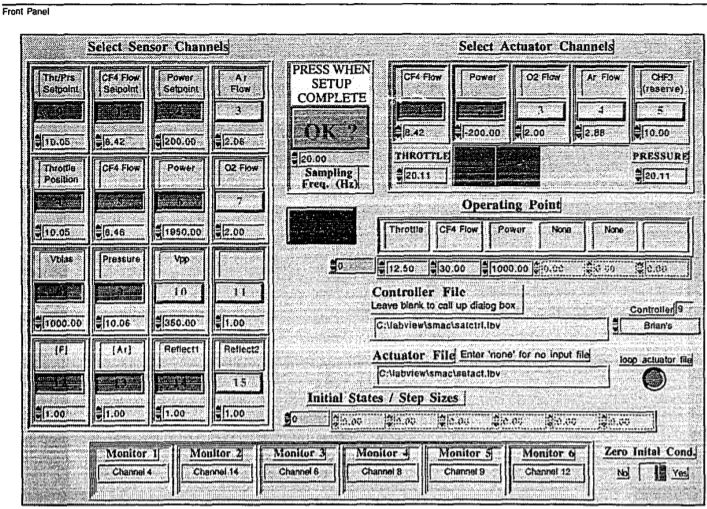
\includegraphics[scale = .7]{Figure 2.13}
	\bf\caption{  LabVIEW Control Setup Panel.}
	\label{fig:2.13}
\end{figure}

\vspace*{3cm}
\setstretch{1.5}
\begin{figure}[H]
	\centering
	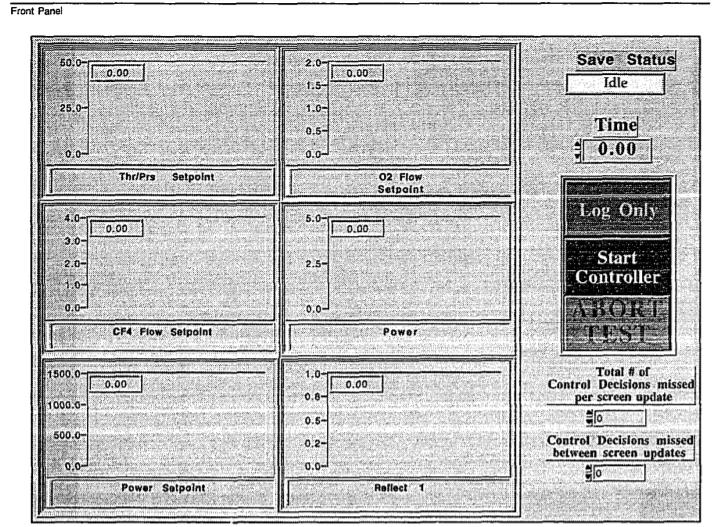
\includegraphics[scale = .8]{Figure 2.14}
	\bf\caption{  LabVIEW Monitor Panel.}
	\label{fig:2.14}
\end{figure}

\newpage

\noindent used to remove high-frequency components from the signals before sampling. Often either Butterworth [78] or Bessel [6] filters are used for this task.

Second-order Butterworth filters were chosen for our system. These were designed around a single operational amplifier as shown in Figure 2.15 [55]. For a Butterworth filter with corner frequency $f_{c}$, the resistors and capacitors are chosen such that


\setstretch{1}
\begin{align}
	f_{c} = \frac{1}{2\pi RC}
\end{align}

\noindent and

\begin{align}
	K=1.586.
\end{align}

\setstretch{1.5}

\noindent The LabVIEW data acquisition system was capable of collecting data at 45 Hz. Therefore, the desired corner frequency was 22.5 Hz. In practice, the resistors and capacitors had to be chosen to correspond to standard values. The filter was implemented with


\setstretch{1}

\begin{align}
	R&=24.1 \text{k}\Omega,\\
	(K-1)R&= 15.9 \text{k}\Omega,
\end{align}

\noindent and

\begin{align}
	C=0.33\mu f.
\end{align}

\noindent These values lead to

\begin{align}
	f_{c}=19.4 \text{Hz}
\end{align}

\noindent and

\begin{align}
	K=1.606.
\end{align}

\begin{figure}[H]
	\centering
	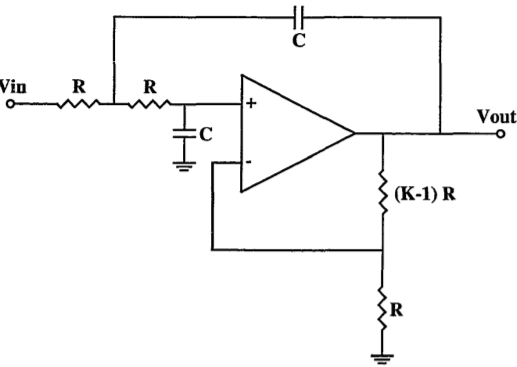
\includegraphics[scale = .7]{Figure 2.15}
	\bf\caption{  Implementation of a lowpass filter.}
	\label{fig:2.15}
\end{figure}

\setstretch{1.5}

The analog input channels on the NB-MIO-16 board were configured with a range of 0 to 10 Volts. If the filters are connected to the input channels at $V_{out}$, the analog channels will saturate at a filter input voltage of $V_{in}$ = 6 V. A voltage divider was added to step the filter gain down to unity. However, because the operational amplifier was powered by ±15 V, $V_{out}$ still saturates at 14.3 V. This saturation occurs at $V_{in}$ = 8.9 V, thus limiting the measurable voltage range to 0 — 8.9 V. In general, this was not a problem for us as most signals remained below 8 volts during normal operation of the system. The exception to this was the optical input signals where it was convenient to have the full 10 volts of range. Recently, the voltage was stepped down at the input stage using a voltage divider and unity gain buffer, as shown in Figure 2.16. This allows the full 0 - 10 V range for the measured inputs. In addition, several of the signals, such as $\text{V}_{bias}$ and power, had ranges between 0 and -10 volts. Therefore, inverting amplifiers were used to bring these voltages into the range of the input channels. Finally, the inverting amplifiers drew enough current on the $\text{V}_{bias}$ channel to actually drop the voltage at the electrode, so a high impedance unity gain buffer was used to isolate the powered electrode from the filter.

\begin{figure}[H]
	\centering
	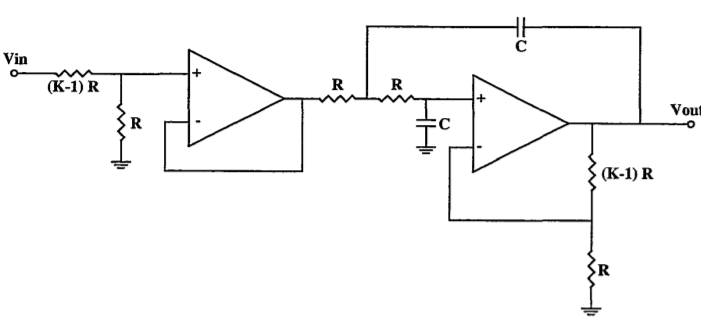
\includegraphics[scale = .7]{Figure 2.16}
	\bf\caption{  Improved lowpass filter.}
	\label{fig:2.16}
\end{figure}
	
	\setstretch{1.5}
\chapter{Dynamic Modeling of the Plasma Generation Process}


\tab In the traditional control of plasma etch tools very few process characteristics are regulated in real time. While the quality of the etch is determined by the etch characteristics presented in Section 1.1.2, real-time in situ measurement of these characteristics is difficult (if not impossible). Therefore, these etch characteristics cannot be used to control the etching process; instead, process recipes are often specified only in terms of equipment setpoints. These setpoints affect the etch characteristics only indirectly through the plasma properties. In some sense, the process engineer is handicapped in that there is only access to equipment inputs, rather than plasma parameters. As the plasma characteristics strongly influence the etch properties, controlling the plasma generation process has the potential for improving the quality of the etch. This forms the basis for the control strategies pursued
in this research.

\setstretch{1}
\section{Control-Oriented Decomposition and Control Strategy.}

\setstretch{1.5}

\tab We begin by “conceptually” decomposing the etch into two separate, but interacting, processes; the plasma generation process (PGP) and the wafer etch process (WEP). This decomposition is shown graphically in Figure 3.1. These sequential processes separate the generation of the important chemical and physical species from the action of etching the surface of the wafer. The inputs to the PGP are the various equipment settings (\textit{e.g.} throttle position, gas composition and flow rates, and applied power); the outputs are the key plasma parameters that are responsible for etching (\textit{e.g.} $V_{bias}$, pressure, ion flux,and the concentration of neutral radicals and polymer precursors\footnote{It is actually the flux of these species to the wafer surface that affects the etching process. However, as was shown in Section 1.2.2, the flux of each species is closely related to its concentration in the bulk plasma.}). The WEP is driven by these plasma parameters and has as outputs the characteristics crucial to etch performance. This decomposition actually represents a physical separation: the PGP represents the bulk plasma, the W EP represents the wafer surface phenomena, and the interface between them is the sheath. It is important to note that there does exist a certain amount of feedback coupling from the wafer surface to the plasma (see, for example, the loading effect in Section 4.2.1). The wafer itself is therefore a disturbance to the plasma generation process.

It is desirable to control the five plasma characteristics shown in Figure 3.1. While there are well established methods of measuring both $V_{bias}$ and pressure, custom sensors are necessary for the measurement of the other characteristics. Unfortunately, of these characteristics, we are presently only able to estimate the concentration of the fluorine radicals. Separate research projects are underway to measure ion current (flux) through rf electrical measurements and polymer precursors using optical emission spectroscopy. For the rest of this dissertation, control of plasma parameters will be limited to $V_{bias}$ pressure, and fluorine concentration ([F]).


The above decomposition of the RIE leads to our control structure. The key idea is to regulate the inputs to the WEP by precisely controlling the outputs of the PGP. This is accomplished by designing a real-time controller for the PG P as shown in Figure 3.2.

\setstretch{1}
\begin{figure}[H]
	\centering
	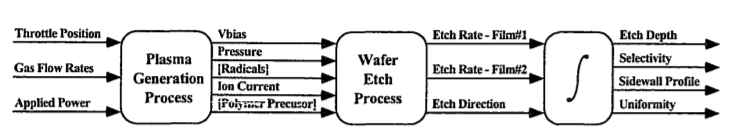
\includegraphics[scale = .7]{Figure 3.1}
	\bf\caption{ Conceptual decomposition of the RIE process.}
	\label{fig:3.1}
\end{figure}

\setstretch{1.5}

\noindent Future research is expected to include the development of a controller around the WEP and a supervisory level controller. The W EP controller will translate desired etch characteristics into setpoints for the PGP control system. The supervisory controller will perform the highlevel cell control functions that include on-line monitoring, diagnostics, and failure recovery as well as post-process analysis of the data for the purposes of sequential optimization, quality control, and so forth. At present, only the PGP controller has been implemented.

There are many merits to this approach:

\begin{itemize}
	\item W ith existing sensor technology, it is very difficult to measure the key wafer etch parameters (selectivity, anisotropy, etc.) in real time during the etch process. (Some of these can be measured in near-real-time.) Therefore, for real-time feedback control,an indirect strategy is necessary.
	
	\item
	Modeling of the etch characteristics is the most difficult part of the problem. With this controller structure, the modeling task may become more tractable. The model for the PGP can be developed first, leading to the development of the real-time plasma controller. Then the modeling task for the WEP would involve relating the effects of the key plasma parameters on the etch performance, which is much more direct than trying to build a single model from the equipment inputs to the etch characteristics.
	
	
	\item The switch from specifying the process recipes in terms of [throttle position, flow rates,
	
	\begin{figure}[H]
		\centering
		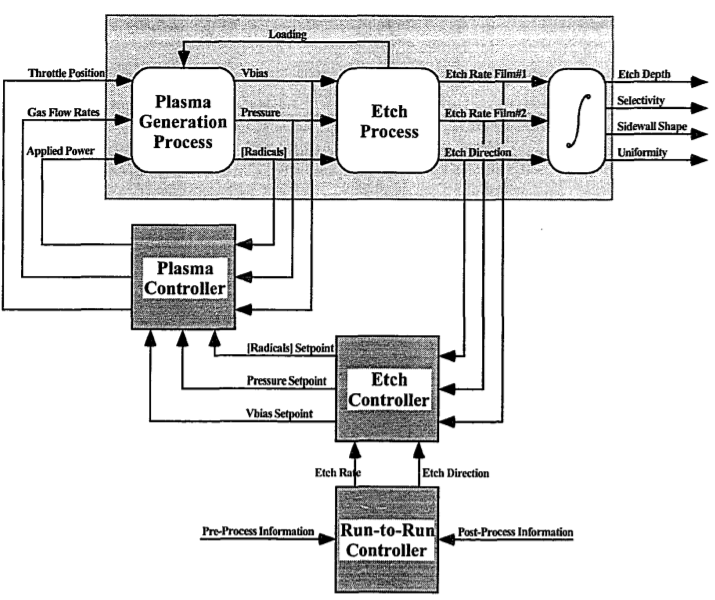
\includegraphics[scale = .7]{Figure 3.2}
		\bf\caption{ Feedback control strategy for th e reactive ion etching process.}
		\label{fig:3.2}
	\end{figure}
	
	power] to [$V_{bias}$, pressure, fluorine concentration] is a significant change of viewpoint. As was seen in Section 1.2.2, these new setpoints are, in many ways, more directly
	connected to the overall etch performance; tightly regulating them should eliminate much of the variance seen in plasma systems. Using plasma characteristics as setpoints may also facilitate the exchange of process recipes between different systems.
	
\end{itemize}

\section{System Identification of the Plasma Generation Process}

\tab The PGP controller is based upon a dynamic model of the plasma generation process. While the PGP is highly nonlinear, a linear model was desired to allow the use of linear control design techniques. Thus, instead of modeling the process dynamics over a wide range of operating conditions, a model was developed that captured the process dynamics in a small region around a give operating point. Two major factors in choosing this operating point were that the etching was in an RIE regime (both chemical and physical) and that the actuators have good authority over the plasma properties. Roughly, the AME-8300 is in an RIE regime for pressures below 50 mTorr and power above 500W.

The nonlinear nature of the throttle valve made it difficult to determine \textit{a priori} its region of highest authority. In the next section, the procedure for determining the throttle settings at which the throttle valve has maximum authority as an actuator is described. This throttle position, along with the $\text{CF}_{4}$ flow rate required to make pressure approximately 20 mTorr and a power of 1000W, defined the operating point used for the modeling of the plasma generation process.

\subsection{Conductance Through the Throttle Valve}

\tab The throttle valve is nonlinear in nature and has different levels of authority at various throttle positions and chamber pressures. Therefore, a set of experiments was devised to find an operating region where the valve was most effective in influencing the pressure.

First, the chamber was sealed from the pump stack by closing the turbo gate valve. The chamber was then filled with $\text{CF}_{4}$ to approximately 85 mTorr, after which the $\text{CF}_{4}$ flow was shut off. The throttle was then set to the desired position; experiments were run at throttle positions

\begin{align}
	\theta = [2.5,5.0,7.5,... , 22.5,25.0] (\% \text{Open}).
\end{align}

\noindent Finally, the turbo gate valve was opened and the pressure was monitored as the chamber was pumped out. A plot of pressure vs. time for the throttle setting $\theta$=12.5 \% Open is shown in Figure 3.3.

Flow can be expressed in terms of a volume per unit time

\setstretch{1}
\begin{align}
	\frac{dV}{dt} = \frac{dn}{dt}\frac{RT_{STP}}{P_{STP}},
\end{align}

\setstretch{1.5}
\noindent where $\frac{dn}{dt}$ is the change in moles of $\text{CF}_{4}$ per unit time, R is the universal gas constant, $T_{stp}$ is standard temperature (298 ° K ) and $P_{stp}$ is standard pressure (760 Torr). The slope of the pressure curve from Figure 3.3 (shown in Figure 3.4 is related to $\frac{dn}{dt}$ by

\setstretch{1}
\begin{align}
	\frac{dn}{dt} = \frac{dP}{dt}\frac{V_{cham}}{RT_{STP}},
\end{align}

\setstretch{1.5}
\noindent where $V_{cham}$ is the volume of the chamber. Thus, the flow through the throttle valve can be found from


\setstretch{1}
\begin{align}
	\frac{dV}{dt} = \frac{dP}{dt}\frac{V_{cham}}{RT_{STP}}.
\end{align}


\begin{figure}[H]
	\centering
	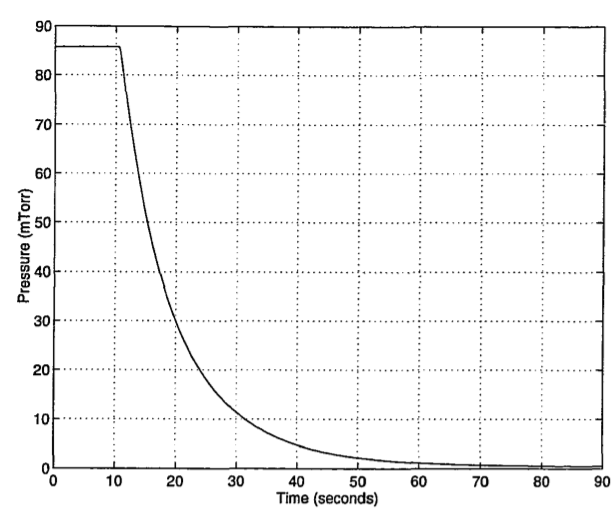
\includegraphics[scale = .6]{Figure 3.3}
	\bf\caption{ Pressure response during conductance experiment.}
	\label{fig:3.3}
\end{figure}

\begin{figure}[H]
	\centering
	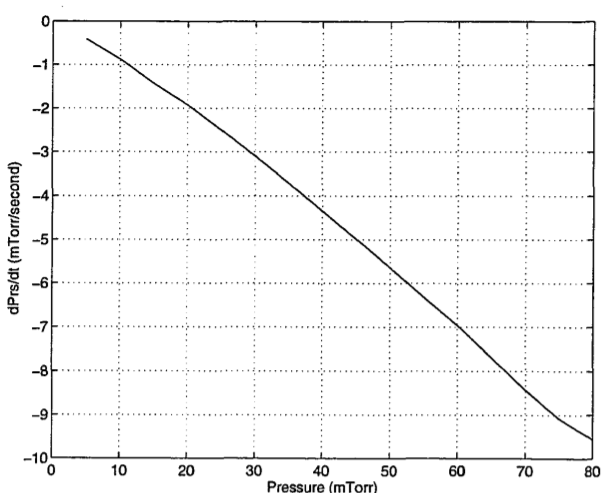
\includegraphics[scale = .6]{Figure 3.4}
	\bf\caption{ dPrs/dt vs. pressure during conductance experiment.}
	\label{fig:3.4}
\end{figure}

\begin{figure}[H]
	\centering
	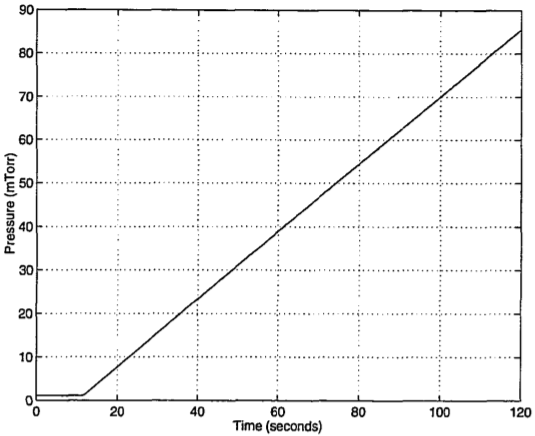
\includegraphics[scale = .75]{Figure 3.5}
	\bf\caption{ Pressure response during volume experiment with a Ar flow of 14 sccm.}
	\label{fig:3.5}
\end{figure}

\setstretch{1.5}
All that remained was to find the volume of the chamber. This was found by isolating the chamber from the pumping stack and measuring the pressure rise at a fix flow rate. The throttle valve could not be used to isolate the chamber, because there is a small (but significant for this experiment) amount of leakage when the valve is fully closed. However, on the AME-8300 there is a turbo gate valve directly above throttle valve; this valve is effective at shutting off flow out of the chamber and was thus used. The throttle valve and the turbo gate valve are very close together, thus using the gate valve does not significantly change the chamber volume. The response of the pressure during this experiment is shown in Figure 3.5.


Prom this data, the pressures $P_{1}$ and $P_{2}$ were recorded at times $t_{1}$ and $t_{2}$, respectively.

From the flow rate ($flw$), the standard volume\footnote{The volume of gas is measured at standard pressure (760 Torr) and temperature (298°K).} of gas added ($V_{added}$) was calculated,

\setstretch{1}
\begin{align}
	V_{added} = flw \times \Delta t
\end{align}

\setstretch{1.5}
\noindent where $\Delta t = t_{2} — t_{1}$. One mole of gas at standard temperature and pressure occupies a volume of $22.4 x 10^{-3}m^{3} [110]$. Next, the number of moles added ($\Delta n$) was computed by


\setstretch{1}
\begin{align}
	\Delta n = \frac{V_{added}}{22.4 x 10^{-3}m^{3}}
\end{align}

\noindent This allowed the volume of the chamber ($V_{cham}$) to be determined by

\begin{align}
	V_{cham} = \frac{\Delta n RT}{\Delta P}
\end{align}

\noindent where $\Delta P = P_{2} — P_{1}$. From this experiment, the chamber volume was calculated to be

\begin{align}
	V_{cham} = 0.211.
\end{align}

\noindent This value was verified by repeating the experiment with different flow rates and gases.

\setstretch{1.5}
Finally, the flow through the throttle valve was calculated using Equation 3.2. Figure 3.6 shows this flow vs. various throttle positions and pressures. From this figure it is seen that the throttle valve has the most authority at settings between 12.5 and 15.0 \%Open. It was determined that for a throttle position of 12.5 \%Open, a $CF_{4}$ flow rate of 30 seem yielded a chamber pressure of 20 mTorr. This operating point was used to develop the model for the plasma generation process and is given again in Table 3.1.

\subsection{Dynamic Model}

\tab The feedback controller design was based on a dynamic model of the plasma generation process. There are several different models that can be used to represent these dynamics. First principle models, such as [64], have the potential of providing a detailed physical


\setstretch{1}
\begin{figure}[H]
	\centering
	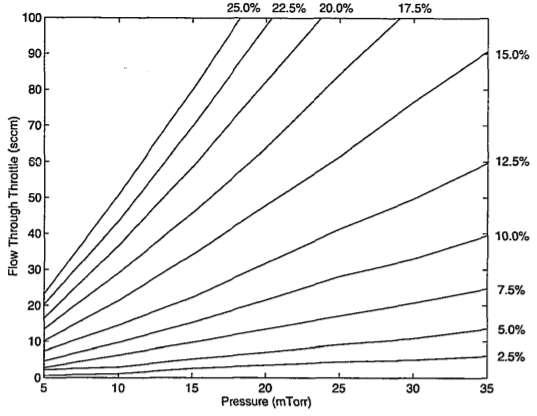
\includegraphics[scale = .75]{Figure 3.6}
	\bf\caption{  Flow through the throttle valve vs. pressure and throttle position.}
	\label{fig:3.6}
\end{figure}

\setstretch{1.5}
\noindent description of the system. Unfortunately, the modeling of plasma and surface reactions is very complex and these models are not well suited for use in real-time feedback control. Another approach is to empirically develop models with input-output data from the system. These models, while easy to develop, only apply to the reactor from which the data was collected. In addition, these models provide little insight into the underlying mechanisms of the process [12]. Many empirical models of plasma etching processes (see, for example, [2,3,57]) only give a static relationship between equipment inputs and etch characteristics. Those used for real-time feedback control need to be dynamic in nature. Between these two extremes are phenomenological models [15]. Phenomenological models attempt to capture only the dominant physical mechanisms and are often empirically tuned to a specific reactor or process.


In this research, 1 have primarily used empirical models of the plasma generation process. The fluorine concentration estimate was based on the physics presented in Section 2.1.3.

\setstretch{1}
\begin{table}[H]
	\centering
	\begin{tabular}{|c|c|}
		\hline
		Throttle Position & 12.5 \%Open \\
		\hline
		$\text{CF}_{4}$ Flow Rate & 30 sccm \\
		\hline
		Applied Power & 1000 W \\
		\hline
	\end{tabular}
	\bf\caption{ Operating point for the plasma generation process model.}
	\label{Table:3.1}
\end{table}

\setstretch{1.5}
However, the estimate itself was empirically related to the inputs of the plasma generation process. The PGP model was based on input-output data collected by separately applying steps to the inputs of our reactor. In the rest of this chapter, 1 present the procedure through which this model was developed.

The initial goal of the control strategy was to use throttle position, $CF_{4}$ flow rate, and power to control the three plasma parameters as shown in Figure 3.2. In order to independently set the steady-state values for all of these properties, the dc gain matrix between the equipment inputs and plasma characteristics must be invertible. This dc gain matrix was found by separately changing each actuator settings allowing the system to settle, and taking the ratio of the change in each plasma property to the change in the input. For the plasma generation process the dc gain matrix had the following form\footnote{The original dc gain matrix upon which conclusions were drawn was not available at the time of writing	of this dissertation. Therefore, presented here is a similar dc gain matrix that was recently collected by Oliver Patterson.}

\setstretch{1}
\begin{align}
	\mbox{\scriptsize$\begin{bmatrix} V_{bias} \\ \text{Pressure} \\ [F]\end{bmatrix} = \begin{bmatrix}	0.330 & -0.254 & 0.740 \\ -1.000 & 1.460 & 0.000 \\ 0.246 & 0.205 & 1.760\end{bmatrix} \begin{bmatrix} \text{Throttle Position} \\ \text{CF}_{4} \text{Flow Rate} \\ \text{Power.}	\end{bmatrix}$}
\end{align}

\setstretch{1.5}
\noindent The invertibility of this matrix is measured by its condition number $\kappa$. The condition number is the ratio of the largest to smallest singular value of the matrix\footnote{For a complete description of singular values and matrix condition numbers see [54].}. The singular values for the dc gain matrix were

\setstretch{1}
\begin{align}
	\sigma = \begin{bmatrix} 1.966 & 1.785 & 0.004626 \end{bmatrix},
\end{align}

\noindent and the condition number was

\begin{align}
	\kappa=425.
\end{align}

\setstretch{1.5}
\noindent This implied that the dc gain matrix was almost singular (noninvertible) and that all three outputs could not be independently controlled. The throttle position and flow inputs are almost redundant; they both primarily affect the plasma through pressure. Of the three outputs, $\text{V}_{bias}$ and fluorine concentration most directly affect the etch characteristics; therefore it was decided to regulate these two plasma properties with the feedback controller. The throttle valve was chosen over the flow controller as a manipulated input to the plasma generation process, because the throttle had a quicker time response and slightly higher command authority. For the remainder of this work, flow rate was held fixed at 30 sccm.

In collecting the data for the step experiments, it was noted that the fluorine concentration measurement was very noisy. One possible method to remove some of this noise is to lower the corner frequency of the lock-in filter; however this could potentially filter out some of the dynamics of the fluorine response. An alternative was to repeat the step experiment several times and average the responses together, thus improving the signal-to-noise ratio while preserving the time response of the signals. The $V_{bias}$ and fluorine concentration responses to the steps in power are shown in Figures 3.7 and 3.8. As can be seen in Figure 3.9, this averaging technique greatly improves the signal-to-noise ratio of the fluorine concentration estimate.

The step response data was then used to determine a model for the plasma generation process. This was done by separately identifying a transfer function for each of the input

\setstretch{1}
\begin{figure}[H]
	\centering
	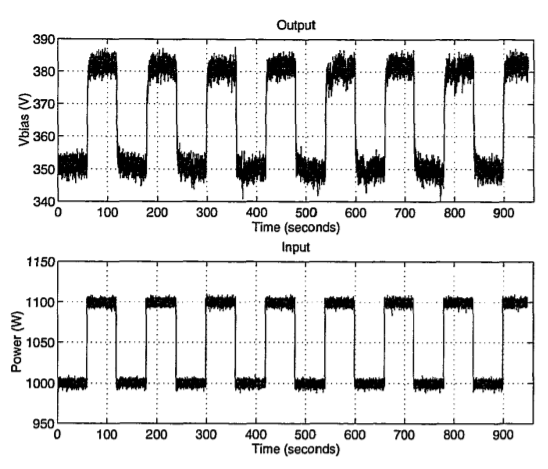
\includegraphics[scale = .7]{Figure 3.7}
	\bf\caption{ $\mathbf{V_{bias}}$ data from power step experiment.}
	\label{fig:3.7}
\end{figure}

\begin{figure}[H]
	\centering
	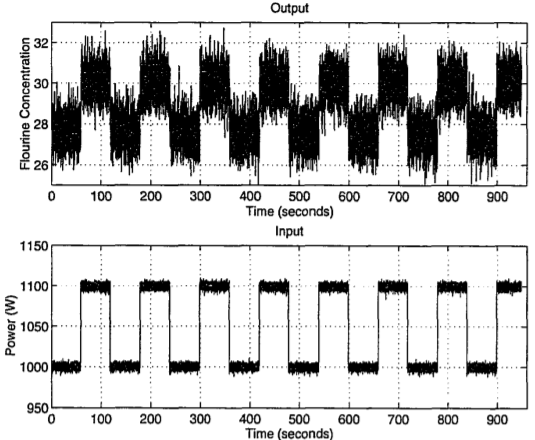
\includegraphics[scale = .7]{Figure 3.8}
	\bf\caption{ Fluorine concentration data power step experiment.}
	\label{fig:3.8}
\end{figure}

\begin{figure}[H]
	\centering
	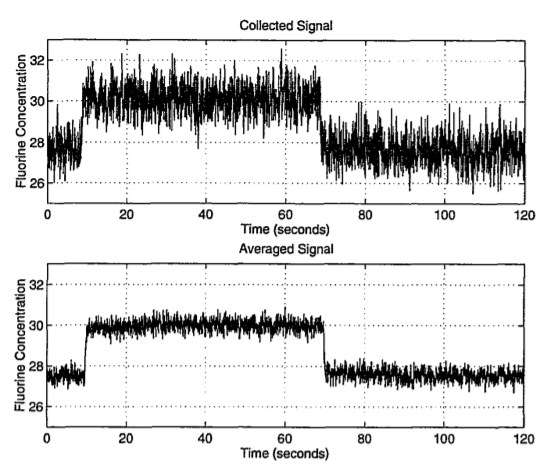
\includegraphics[scale = .7]{Figure 3.9}
	\bf\caption{ Noise reduction due to averaging of [F] signal.}
	\label{fig:3.9}
\end{figure}

\setstretch{1.5}
\noindent output pairs. There are several different linear model structures that can be used to capture the dynamics of a system. A complete description of the various model structures can be
found in [69,98]. Each of these model structures is characterized by a number of parameters which are empirically determined through a least squares optimization; this process is known
as system identification. Initially, several different model structures were compared; the Auto-Regressive Moving Average with eXogenous input (ARMAX) model provided the best fit to the experimental data and was used to model the plasma generation process. In practice, it is often useful to overparameterize the model [69]; this may lead to better fits with the experimental data. The extraneous parameters can later be removed. The system
identification algorithms used in this dissertation generate discrete-time models which were then converted to continuous time for controller design.

\setstretch{1}
\begin{table}[H]
	\centering
	\renewcommand{\arraystretch}{2}
	\begin{tabular}{|c|c|c|c|}
		\hline
		Order & Transfer Function & DC Gain & Mean Square Error \\
		\hline 
		First Order & \large{$\frac{0.3726}{s+1.195}$} & 0.3118 & 0.772 \\
		\hline
		Second Order & \large{$\frac{0.6593(s+7.543)}{(s+1.085)(s+14.639)}$} & 0.3131 & 0.739 \\
		\hline
		Third Order & \large{$\frac{0.4679(s+0.467)(s+1.9828)}{(s+0.362)(s+1.923)(s+1.9832)}$} & 0.3136 & 0.593 \\
		\hline
	\end{tabular}
	\renewcommand{\arraystretch}{1}
	\bf\caption{ Transfer functions from power to $\mathbf{V_{bias}}$ Power to $\mathbf{V_{bias}}$ Response}
	\label{Table:3.2}
\end{table}

\setstretch{1.5}
As can be seen from this Table and the simulated step responses in Figure 3.11, the third order model had the best fit to the experimental data. The differences in the models can be seen from the Bode plots in Figure 3.12. Note that the third order model has an almost pole-zero cancelation; removing the pole-zero pair yields a second order model that fits the experimental data better than the second order model obtained 

\setstretch{1}
\begin{figure}[H]
	\centering
	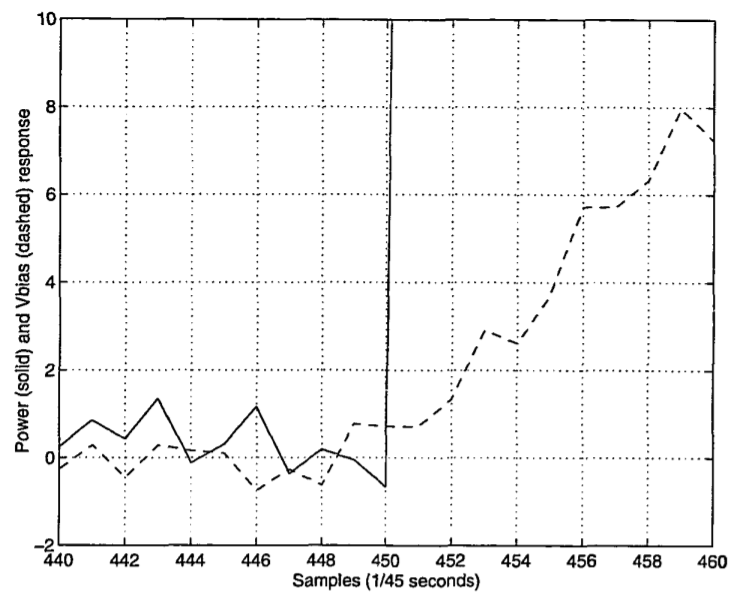
\includegraphics[scale = 0.55]{Figure 3.10}
	\bf\caption{ Delay in response of $\mathbf{V_{bias}}$ to a step in power.}
	\label{fig:3.10}
\end{figure}

\setstretch{1.5}
\noindent directly from the identification. In principle, the second order model obtained directly should be optimal; however, the parameters of this model are obtained by the gradient search technique and thus may have converged only to a local minimum. Therefore, by removing the pole-zero pair for the third order model, the following second order transfer function for the response from power to $V_{bias}$ was found to be


\setstretch{1}
\begin{align}
	G_{vp}(s) = \frac{0.468(s+0.467)}{(s+0.362)(s+1.923)}.
\end{align}

\setstretch{1.5}
\noindent\textbf{Power to Fluorine Concentration Response}

Next, the transfer function for the response from power to estimated fluorine concentration was identified. As with the response of $V_{bias}$ to this input, the fluorine concentration
also responds with a delay of only one sample. This can be seen in Figure 3.13. The armcix command was again used to identify first, second, and third


\setstretch{1}

\begin{figure}[H]
	\centering
	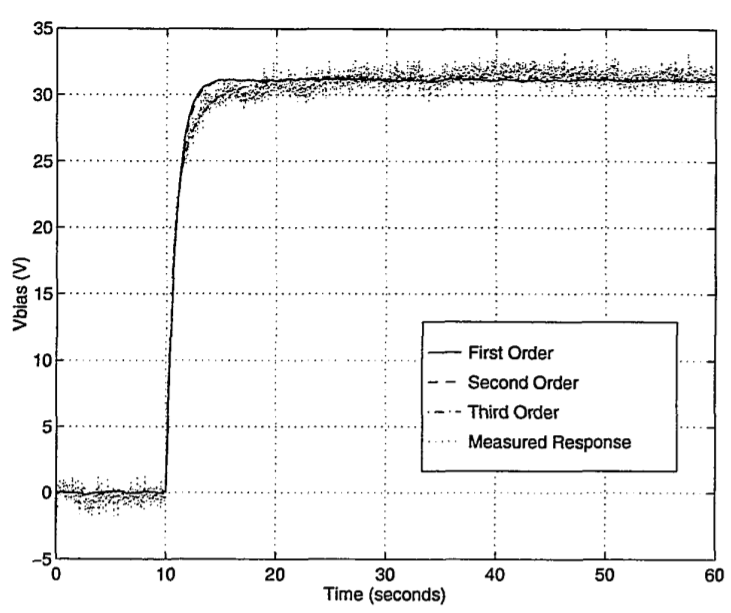
\includegraphics[scale = .55]{Figure 3.11}
	\bf\caption{ Step response: Power to $\mathbf{V_{bf}}$.}
	\label{fig:3.11}
\end{figure}

\begin{figure}[H]
	\centering
	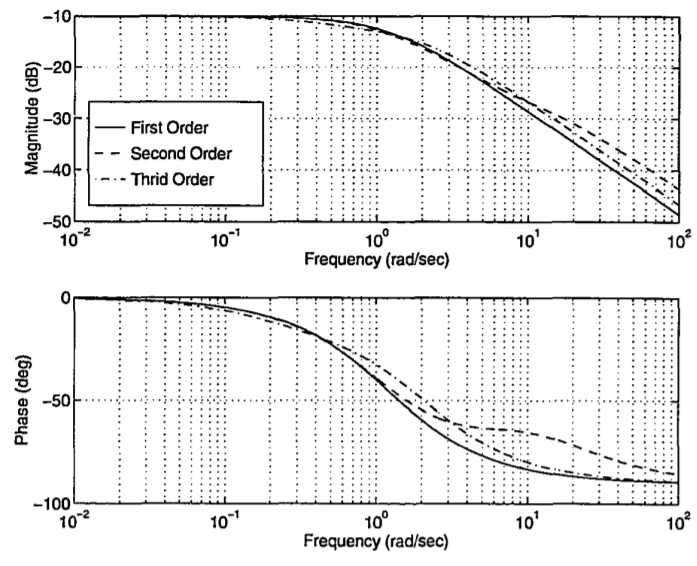
\includegraphics[scale = .55]{Figure 3.12}
	\bf\caption{ Bode plot: Power to $\mathbf{V_{bias}}$.}
	\label{fig:3.12}
\end{figure}

\begin{figure}[H]
	\centering
	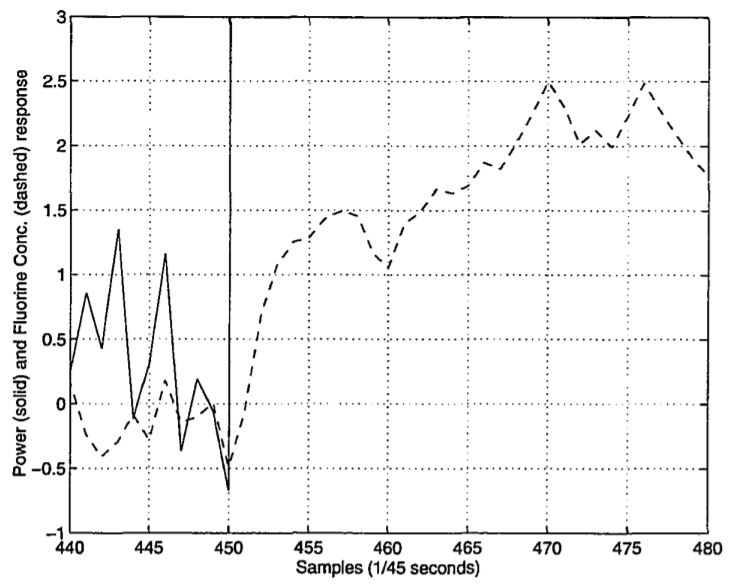
\includegraphics[scale = .55]{Figure 3.13}
	\bf\caption{  Delay in response of fluorine concentration to a step in power.}
	\label{fig:3.13}
\end{figure}

\begin{table}[H]
	\centering
	\renewcommand{\arraystretch}{2}
	\begin{tabular}{|c|c|c|c|}
		\hline
		Order & Transfer Function & DC Gain & Mean Square Error \\
		\hline 
		First Order & \large{$\frac{0.4314}{s+27.61}$} & 0.0245 & 0.248 \\
		\hline
		Second Order & \large{$\frac{0.4598(s+6.275)}{(s+2.662)(s+44.07)}$} & 0.0246 & 0.230 \\
		\hline
		Third Order & \large{$\frac{0.5630(s+5.54)(s+34.47)}{(s+2.48)(s+36.29)(s+48.23)}$} & 0.0246 & 0.230 \\
		\hline
	\end{tabular}
	\renewcommand{\arraystretch}{1}
	\bf\caption{ Transfer functions from power to fluorine concentration.}
	\label{Table:3.3}
\end{table}

\setstretch{1.5}
\noindent  order models; these are given in Table 3.3. A comparison of the step responses of each of these models, seen in Figure 3.14, shows that both the second and third order transfer functions do an adequate job of fitting the measured response. Indeed, as shown in Figure 3.15, the Bode plots of these models are very similar. This is a result of a near pole-zero cancelation in the third order model. It was concluded that that was an adequate representation of the response fluorine concentration to a step in power. Though the pole at -44.07 has no significant effect on the response, it is retained to keep
the transfer function strictly proper. This simplifies the controller design by providing a model with no direct feedthrough term.

\setstretch{1}
\begin{align}
	G_{vp}(s) = \frac{0.460(s+6.28)}{(s+2.66)(s+44.07)}.
\end{align}

\begin{figure}[H]
	\centering
	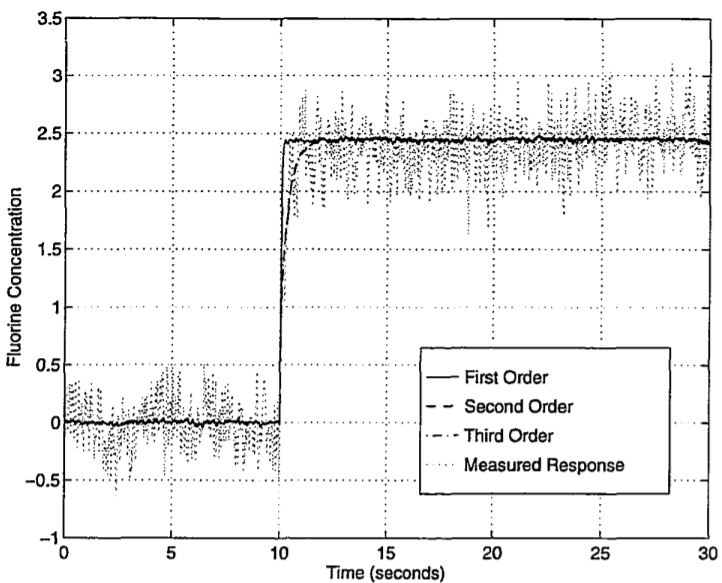
\includegraphics[scale = .55]{Figure 3.14}
	\bf\caption{  Step response: Power to fluorine concentration.}
	\label{fig:3.14}
\end{figure}

\setstretch{1.5}

\noindent \textbf{Throttle Position to $\mathbf{V_{bias}}$ Response}

The response of the system to a step change in throttle position was identified next. Determining the pure time delay for this response was more difficult than in the previous cases. There was a gradual initiation in the response and this coupled with noise made it difficult determine the time delay. Therefore to assist in calculating this delay, a line was drawn tangent to the rising slope of the response and extended back through the x-axis, as shown in Figure 3.16. From a close-up view of the region where this line intercepts the axis (Figure 3.17), the delay was determined to be approximately 28 samples or 0.622 seconds.

\setstretch{.75}
\begin{figure}[H]
	\centering
	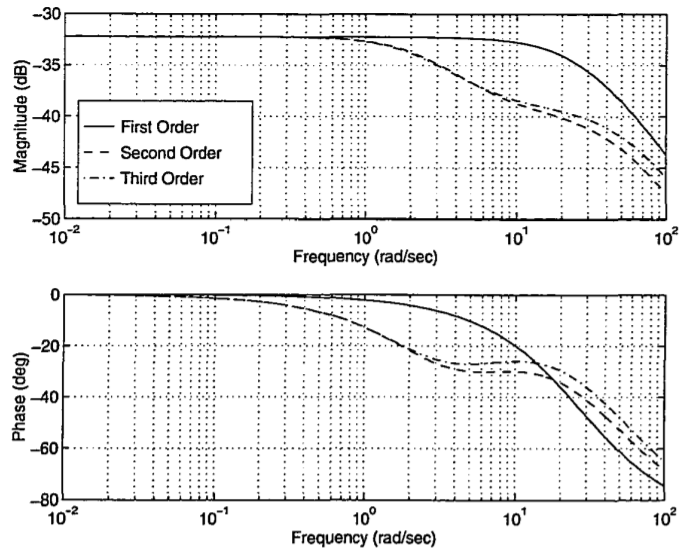
\includegraphics[scale = .5]{Figure 3.15}
	\bf\caption{  Bode plot: Power to fluorine concentration.}
	\label{fig:3.15}
\end{figure}

\begin{table}[H]
	\centering
	\renewcommand{\arraystretch}{2}
	\begin{tabular}{|c|c|c|c|}
		\hline
		Order & Transfer Function & DC Gain & Mean Square Error \\
		\hline 
		First Order & \large{$\frac{2.80}{s+0.174}$} & 16.08 & 0.614 \\
		\hline
		Second Order & \large{$\frac{2.98(s+3.48)}{(s+0.173)(s+3.72)}$} & 16.08 & 0.618 \\
		\hline
		Third Order & \large{$\frac{-0.768(s+2.35)(s-68.46)}{(s+0.175)(s+2.58)(s+16.30)}$} & 16.10 & 0.611 \\
		\hline
	\end{tabular}
	\renewcommand{\arraystretch}{1}
	\bf\caption{ Transfer functions from throttle position to $\mathbf{V_{bias}}$}
	\label{Table:3.4}
\end{table}

\setstretch{1.5}
The various order identified models are shown in Table 3.4. The dominant pole in each of these models was around s = —0.174. Indeed both the step responses (Figure 3.18 and Bode plots 3.19 show similar responses for all of these models. Thus, for this input-output pair the transfer function model was found to be

\setstretch{1}
\begin{align}
	G_{vt}(s)=\frac{2.80e^{-0.622\tau}}{s+0.174},
\end{align}

\noindent where $e^{-0.622\tau}$ represents the time delay of $\frac{28}{45}$ seconds.

\setstretch{1}
\begin{figure}[H]
	\centering
	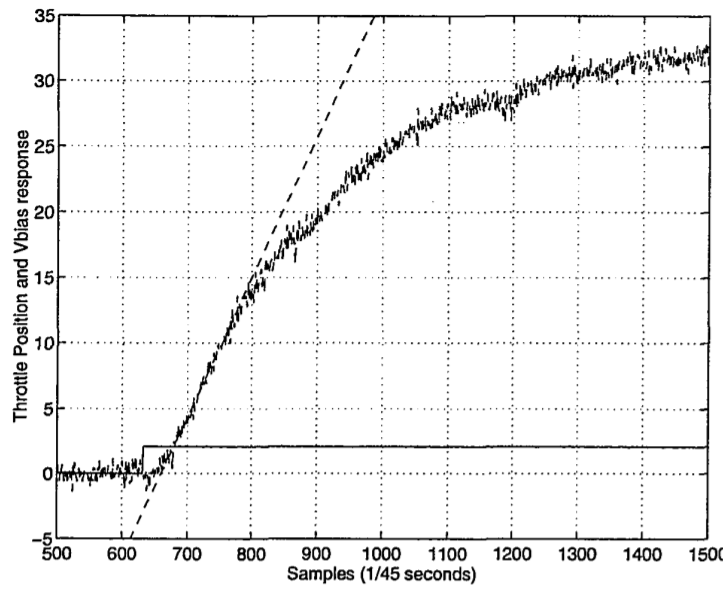
\includegraphics[scale = .5]{Figure 3.16}
	\bf\caption{  Delay in response of $\mathbf{V_{bias}}$ to a step in throttle position.}
	\label{fig:3.16}
\end{figure}

\begin{figure}[H]
	\centering
	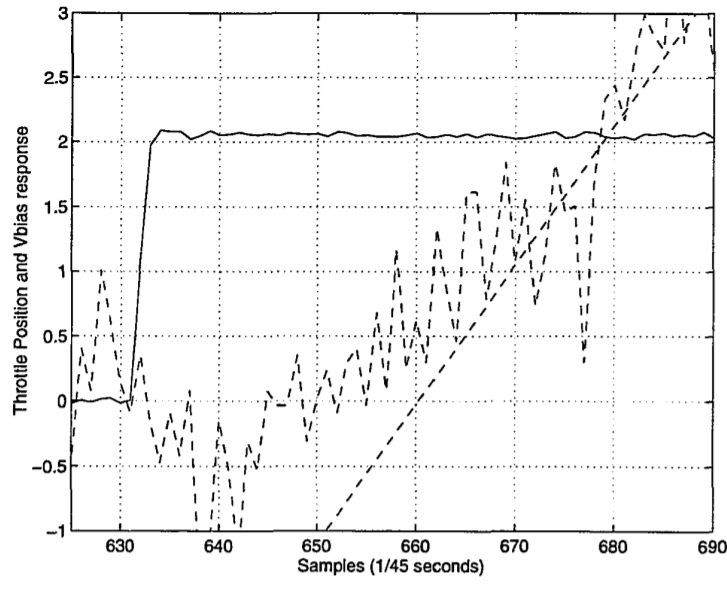
\includegraphics[scale = .5]{Figure 3.17}
	\bf\caption{  Detailed view of the delay in response of $\mathbf{V_{bias}}$ to a step throttle position.}
	\label{fig:3.17}
\end{figure}

\begin{figure}[H]
	\centering
	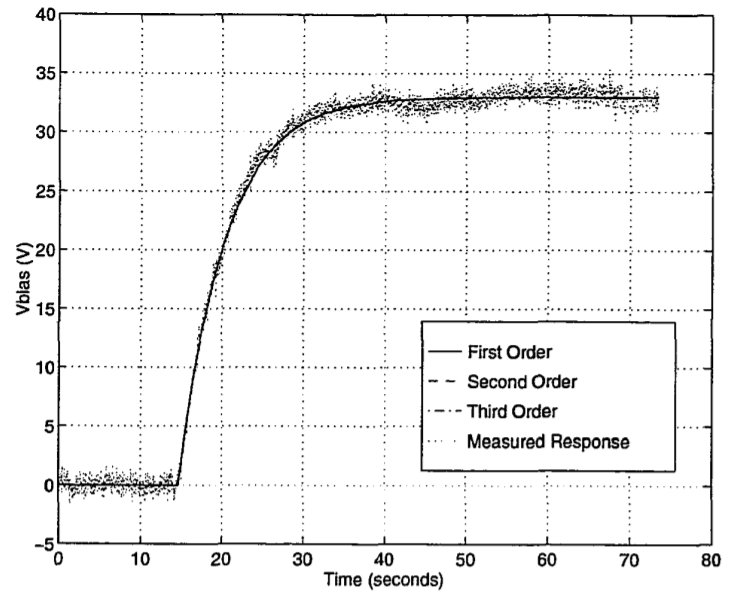
\includegraphics[scale = .5]{Figure 3.18}
	\bf\caption{  Time response: Throttle position to $\mathbf{V_{bias}}$.}
	\label{fig:3.18}
\end{figure}

\begin{figure}[H]
	\centering
	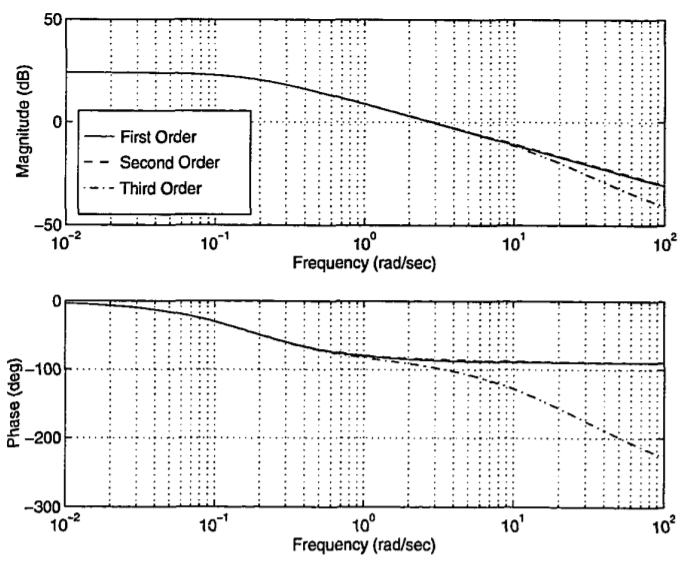
\includegraphics[scale = .5]{Figure 3.19}
	\bf\caption{  Bode plot: Throttle position to $\mathbf{V_{bias}}$.}
	\label{fig:3.19}
\end{figure}

\begin{figure}[H]
	\centering
	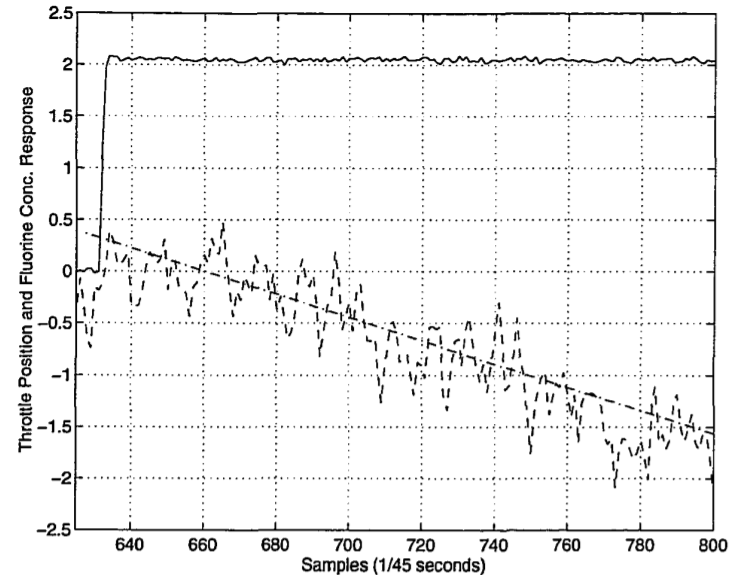
\includegraphics[scale = .5]{Figure 3.20}
	\bf\caption{  Delay in response of fluorine concentration to a step in throttle position. }
	\label{fig:3.20}
\end{figure}

\setstretch{1.5}
\noindent \textbf{Throttle Position to Fluorine Concentration Response}

The final transfer function to be identified was for the response of fluorine concentration to a step in throttle position. The time delay was determined in the same manner as the one for the $V_{bias}$ response. As is shown in Figures 3.20 and 3.21, the delay is again approximately 28 samples. The identified transfer functions are shown in Table 3.5. In this case, the second and third order models accurately simulate 

\setstretch{1}
\begin{table}[H]
	\centering
	\renewcommand{\arraystretch}{2}
	\begin{tabular}{|c|c|c|c|}
		\hline
		Order & Transfer Function & DC Gain & Mean Square Error \\
		\hline 
		First Order & \large{$\frac{-3.98}{s+2.03}$} & -1.93 & 0.728 \\
		\hline
		Second Order & \large{$\frac{4.03(s-3.56)}{(s+0.204)(s+33.38)}$} & -2.10 & 0.300 \\
		\hline
		Third Order & \large{$\frac{3.91(s+2.42)(s-3.61)}{(s+0.204)(s+2.39)(s+33.33)}$} & -2.10 & 0.300 \\
		\hline
	\end{tabular}
	\renewcommand{\arraystretch}{1}
	\bf\caption{ Transfer functions from throttle position to fluorine concentration.}
	\label{Table:3.5}
\end{table}

\begin{figure}[H]
	\centering
	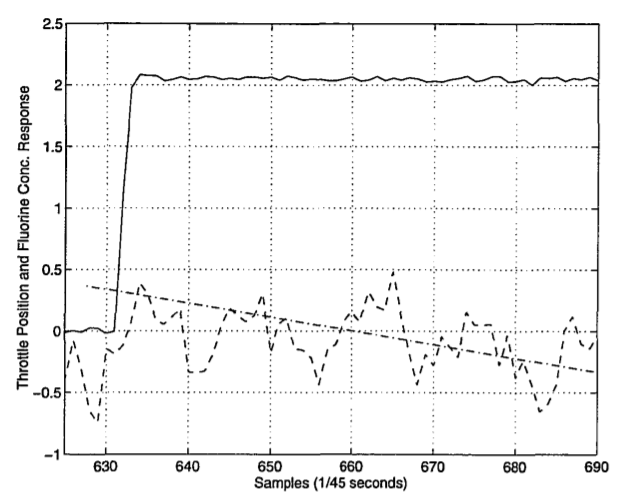
\includegraphics[scale = .5]{Figure 3.21}
	\bf\caption{  Detailed view delay in response of fluorine concentration to a step in throttle position.}
	\label{fig:3.21}
\end{figure}

\setstretch{1.5}
\noindent the fluorine response. This is shown in Figure 3.23. Likewise, both of these models have similar Bode plots (Figure 3.22).
In each model, the pole at $s = —0.204$ dominates the other poles and zeros. Therefore, including the time delay, the model was reduced to


\setstretch{1}
\begin{align}
	G_{Ft}(s) = \frac{-0.428e^{-0.622\tau}}{s+0.204}
\end{align}

\setstretch{1.5}

\noindent\textbf{Full Model}

The full system was modeled by combining the four individual transfer function (Equations 3.12, 3.13, 3.14, and 3.15) into a 2 x 2 transfer function matrix.

\setstretch{1}
\begin{figure}[H]
	\centering
	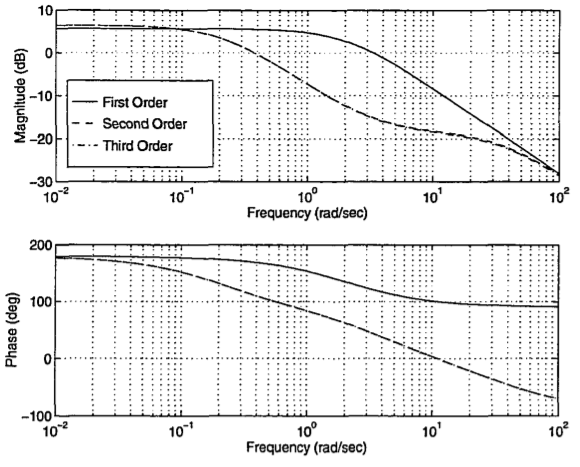
\includegraphics[scale = .6]{Figure 3.22}
	\bf\caption{  Bode plot: Throttle position to fluorine concentration.}
	\label{fig:3.22}
\end{figure}

\begin{figure}[H]
	\centering
	\includegraphics[scale = .6]{Figure 3.23}
	\bf\caption{  Time response: Throttle position to fluorine concentration.}
	\label{fig:3.23}
\end{figure}

\begin{align}
	\renewcommand\arraystretch{2} \begin{bmatrix} V_{bias} \\ [F] \end{bmatrix} = \begin{bmatrix} \frac{2.80e^{-0.622\tau}}{s+0.174} & \frac{0.468(s+0.467)}{(s+0.362)(s+1.923)} \\ \frac{-0.428e^{-0.622\tau}}{s+0.204} & \frac{0.460(s+6.28)}{(s+2.66)(s+44.07)}  \end{bmatrix} \begin{bmatrix} \text{Throttle Position} \\ \text{Power} \end{bmatrix}
\end{align}

\setstretch{1.5}

\section{Model Validation}

\tab In order to determine if the 2 x 2 transfer function model was a good approximation of the physical system, an experimental test was performed. The model was identified by exciting the system with only one actuator at a time; in the real system, it is of course possible to vary both the throttle position and power simultaneously. In principle, our linear model should predict the response to small simultaneous variations in the actuators with the same fidelity as it predicts the response to individual variations. In practice, however, the model may fail to accurately describe the system response due to neglected nonlinearities. To test the fidelity of our model’s ability to describe simultaneous actuator variations, two simultaneous pseudo random binary signals (PRBS) [98] were applied to the actuators; these are shown in Figure 3.24. The PRBS applied to the throttle position was given a slower switching rate because the dynamics associated with the throttle were slower than those associated with the power input. The response of the model and the actual system, as well as the error between them, is plotted in Figure 3.25 for the $V_{bias}$ signal. As can be seen from this plot, except for a small bias in the response, the model accurately represents the dynamics of the system; a tentative explanation for this bias is that it is due to nonlinearity. A similar comparison for fluorine concentration is shown in Figure 3.26. In this case the resulting error shows very little bias, though the signal-to-noise ratio is very poor.

\setstretch{1}
\begin{figure}[H]
	\centering
	\includegraphics[scale = .6]{Figure 3.24}
	\bf\caption{ PRBS applied in model validation experiment.}
	\label{fig:3.24}
\end{figure}

\begin{figure}[H]
	\centering
	\includegraphics[scale = .6]{Figure 3.25}
	\bf\caption{  Comparison of actual and simulated $\text{V}_{bias}$ response to simultaneous PRBS inputs.}
	\label{fig:3.25}
\end{figure}

\begin{figure}[H]
	\centering
	\includegraphics[scale = .75]{Figure 3.26}
	\bf\caption{ Comparison of actual and simulated fluorine concentration response to simultaneous PRBS inputs.}
	\label{fig:3.26}
\end{figure}
	
	\setstretch{1.5}
\chapter{Etch Rate Control and Disturbance Rejection}

\tab The principle aim of this research was to show how modern real-time control techniques can be used to improve the quality of the reactive ion etching process. It was based on the hypothesis that regulating plasma properties, instead of simply setting equipment inputs, provides tighter control of important etch characteristics. In this chapter, the ability of this control strategy to attenuate the effect of exogenous perturbations on etch rate was explored. First, a controller for the plasma generation process was designed based upon the dynamic model developed in Section 3.2. This controller allowed the operator to specify process condition in terms of plasma properties ($\text{V}_{bias}$ and fluorine concentration), as opposed to the standard industrial practice of only using feedback control to regulate pressure (in this case, gas flow rates and applied power are set to constant values). The PG P controller is then compared to standard practice in its ability to reject disturbances to etch rate.

\section{Plasma Generation Process Controller}

\tab The plasma generation process controller was designed to regulate the plasma properties by manipulating the inputs to the AME-8300. It was desired that the plasma setpoints be held at constant values during the etch; therefore, the controller was designed to have zero steady-state error in tracking constant reference signals. At the process conditions used for this research, the duration of a typical etch was at least 900 seconds. It was decided that a settling time of approximately 25 seconds was sufficient for an etch of this length.


In meeting these performance objectives, there were a number of constraints that limited the bandwidth of the controller. These included the time delay in the response of the system to changes in the throttle position, the noise on the fluorine concentration estimate, and the throttle nonlinearity. Of these, the throttle nonlinearity was dominant and thus the overshoot in the throttle valve response was limited to 20\%.

\subsection{Controller Design}

\tab The design of the plasma generation process controller was done using a state space representation\footnote{in the state space representation, the system is modeled by a first order matrix differential equation. Complete details of the state space representation can be found in [17].} of the transfer function matrix from Equation 3.16. The pure time delay in the system’s response to changes in throttle position was represented by a Fade approximation. Both first and second order approximations were compared. The controller bandwidth was expected to be below 1 radian/second. Since, as shown in Figure 4.1, the phase lag of both approximations was similar out to the expected controller bandwidth, it was decided that the first order approximation was sufficient. Therefore, the delay was represented as Using this approximation, a Simulink\footnote{Simulink is a block-diagram-based simulation package that is part of Matlab.} model

\setstretch{1}
\begin{align}
	e^{-s\tau} \approx \frac{-\frac{\tau}{2} s +1}{\frac{\tau}{2} s +1}
\end{align}

\setstretch{1.5}
\noindent of the dynamics from throttle position and
power to $\text{V}_{bias}$ and [F] was developed. This is shown in Figure 4.2. In order to equate changes in the inputs and outputs, each was scaled by its nominal value. For convenience,

\setstretch{1}
\begin{figure}[H]
	\centering
	\includegraphics[scale = .6]{Figure 4.1}
	\bf\caption{ Phase lag from the Fad\'{e} approximations o f time delay.}
	\label{fig:4.1}
\end{figure}

\begin{figure}[H]
	\centering
	\includegraphics[scale = .6]{Figure 4.2}
	\bf\caption{ Simulink block diagram: plasma generation process model.}
	\label{fig:4.2}
\end{figure}

\noindent the Simulink command linmod [73] was used to create the state space representation

\begin{align*}
	\dot x(t) = A_{p} x(t) + B_{p}u(t)
\end{align*}

\begin{align}
	y(t) = C_{p} x(t) + D_{p}u(t)
\end{align}

\noindent where $u(t)$ are the process inputs, $y(t)$ are the process outputs, $x(t)$ are the states of the model, and

\begin{align}
	\renewcommand\arraystretch{2} A_{p} &= \begin{bmatrix}
		-8.436 & -1.304 & 0 & 0 & 0 & 0 & 0 \\ 1.304 & 0 & 0 & 0 & 0 & 0 & 0 \\ 0 & 0 & -0.2221 & 0 & 0 & 0 & 6.429 \\ 0 & 0 & 0 & -145.4 & -5.239 & 0 & 0 \\ 0 & 0 & 0 & 5.239 & 0 & 0 & 0 \\ 0 & 0 & 0 & 0 & 0 & -0.167 & 6.429 \\ 0 & 0 & 0 & 0 & 0 & 0 & -3.214 
	\end{bmatrix} \\
	B_{p} &= \begin{bmatrix}
		0 & 1000 \\ 0 & 0 \\ -12.5 & 0 \\ 0 & 1000 \\ 0 & 0 \\ -12.5 & 0 \\ 12.5 & 0
	\end{bmatrix} \\
	C_{p} &= \begin{bmatrix}
		0 & 0 & 0 & 0.0983 & 0.0043 & 0.0055 & 0 \\ 0.0019 & 0.0005 & -0.0044 & 0 & 0 & 0 & 0
	\end{bmatrix} \\
	D_{p} &= \begin{bmatrix}
		0 & 0 \\ 0 & 0
	\end{bmatrix}
\end{align}

\setstretch{1.5}
\noindent This model of the system dynamics is known as the p la n t For the rest of this dissertation, the time dependence will be dropped from this notation and it should be understood that the inputs $u$, states $x$ , and outputs $y$ are all functions of time. Also, since $D_{p}=0$, it does not enter into the calculations presented below.


The most important performance objective was to have zero steady-state error in tracking plasma setpoints. This was accomplished by using integral control [25]. The first step in the design was to augment the system with integrators. A set of states $q$, equal to the integral of the error between the plant output and the desired output $r$, was defined by

\setstretch{1}
\begin{align}
	\dot q = y-r.
\end{align}

\noindent Augmenting the system in Equation 4.2 with these states, the new plant became

\begin{align*}
	\begin{bmatrix}
		\dot x \\ \dot q
	\end{bmatrix} &=
	\myunderbrace{\begin{bmatrix}
			A_{p} & 0 \\ C_{p} & 0 
	\end{bmatrix}}{A_{m}} 
	\begin{bmatrix}
		x \\ q
	\end{bmatrix} + 
	\myunderbrace{\begin{bmatrix}
			B_{p} \\ 0
	\end{bmatrix}}{B_{m}} u +
	\myunderbrace{\begin{bmatrix}
			0 \\ -I
	\end{bmatrix}}{G_{m}} r,
\end{align*}

\begin{align}
	y &= 
	\myunderbrace{\begin{bmatrix}
			C_{p} & 0 
	\end{bmatrix}}{C_{m}} 
	\begin{bmatrix} 
		x \\ q
	\end{bmatrix}.
\end{align}

\noindent To simplify notation, we define the augmented state vector $ x_{m} = \begin{bmatrix}
	x \\ q
\end{bmatrix}$ and rewrite Equation 4.8 as

\begin{align*}
	\dot x = A_{m}x_{m} + B_{m}u + G_{m} r
\end{align*}

\begin{align}
	y = C_{m} x_{m} . 
\end{align}

\begin{figure}[H]
	\centering
	\includegraphics[scale = .75]{Figure 4.3}
	\bf\caption{ State feedback diagram.}
	\label{fig:4.3}
\end{figure}

\setstretch{1.5}
In selecting the feedback gains, it was first assumed that the states $x_{m}$ were measurable and that the controlled inputs had the form


\setstretch{1}
\begin{align}
	u = -Kx_{m},
\end{align}

\noindent where

\begin{align}
	K = \begin{bmatrix}
		K_{1} & K_{2}
	\end{bmatrix}
\end{align}

\setstretch{1.5}
was the state feedback gain as shown in Figure 4.3. This state feedback gain was found by solving the linear quadratic regulator (LQR) problem. Briefly, in the LQR problem the controller gain $K$ is found by minimizing the cost function


\setstretch{1}
\begin{align}
	J = \int_{0}^{\infty} \left( x'Qx+u'Ru \right) dt,
\end{align}

\setstretch{1.5}
subject to the system in Equation 4.9 and the control input from Equation 4.10. In this equation, $Q$ is a matrix of weights for the states and $R$ is a matrix of weights for the inputs. Complete details of the LQR problem can be found in [4]. In this research, the weight
matrix for the states had the form

\setstretch{1}
\begin{align}
	\renewcommand\arraystretch{1.5} Q = \begin{bmatrix}
		\alpha C'_{p}C_{p} & 0 \\ 0 & Q_{p}
	\end{bmatrix}
\end{align}

\setstretch{1.5}
\noindent where $\alpha$ was a scalar and $Q_{q}$ was a diagonal matrix of the weights for each integrator state. The input weight matrix $R$ was a diagonal matrix of weights for each individual input.

Applying the control inputs from Equation 4.10 to the system in Equation 4.9 yields the following closed loop system


\setstretch{1}
\begin{align*}
	\dot x_{m} = \left( A_{m} - B_{m}K \right) x_{m} + G_{m} r
\end{align*}

\begin{align}
	y = C_{m}x_{m}.
\end{align}

\setstretch{1.5}
\noindent Parameters for the weight matrices were chosen and the closed loop system simulated to determine if the performance objectives and design constraints were satisfied. After several iterations, the following parameters were settled upon

\setstretch{1}
\begin{align}
	\alpha &= 1,\\
	Q_{p} &= \begin{bmatrix}
		0.6 & 0.0 \\ 0.0 & 0.5 
	\end{bmatrix},
\end{align}

\noindent and

\begin{align}
	R = \begin{bmatrix}
		4.0 & 0.0 \\ 0.0 & 3.0 
	\end{bmatrix}.
\end{align}

\setstretch{1.5}
\noindent The Iqr command from the Matlab Control Systems Toolbox [40] was used to calculate the state feedback gains

\setstretch{1}
\begin{align}
	\renewcommand\arraystretch{1.5}
	K_{1} = \begin{bmatrix}
		0.000 & 0.000 & 0.006 & 0.000 & 0.001 & 0.004 & 0.019 \\ 0.000 & 0.000 & -0.002 & 0.011 & 0.001 & 0.005 & 0.004
	\end{bmatrix}
\end{align}

\begin{figure}[H]
	\centering
	\includegraphics[scale = .6]{Figure 4.4}
	\bf\caption{ Simulated response of closed loop system to a step in $\text{V}_{bias}$}
	\label{fig:4.4}
\end{figure}

\noindent and

\begin{align}
	K_{2} = \begin{bmatrix}
		0.162 & -0.321 \\ 0.406 & 0.171
	\end{bmatrix}.
\end{align}

\setstretch{1.5}
\noindent Figure 4.4 shows the simulated response of the plasma to a step change in the $\text{V}_{bias}$ command. The corresponding responses of the actuators are shown in Figure 4.5. Likewise, the plasma and actuator responses for a step change in the fluorine concentration setpoint are shown in Figures 4.6 and 4.7.

\noindent\textbf{Observer Design}

In practice, the states of the system are not available for feedback, therefore they must be estimated. Actually, only the states of the plant $x$ needed to be estimated, as the integrated error states $q$ are calculated in the controller. The true system has disturbances

\setstretch{1}
\begin{figure}[H]
	\centering
	\includegraphics[scale = .6]{Figure 4.5}
	\bf\caption{ Simulated response of actuators to a step in $\text{V}_{bias}$.}
	\label{fig:4.5}
\end{figure}

\begin{figure}[H]
	\centering
	\includegraphics[scale = .6]{Figure 4.6}
	\bf\caption{ Simulated response of closed loop system to a step in fluorine concentration.
	}
	\label{fig:4.6}
\end{figure}

\begin{figure}[H]
	\centering
	\includegraphics[scale = .75]{Figure 4.7}
	\bf\caption{ Simulated response of actuators to a step in fluorine concentration.}
	\label{fig:4.7}
\end{figure}

to the process and noise in the measurements. This was represented by

\begin{align*}
	\dot x(t) = A_{p}x+B_{p}u+v
\end{align*}

\begin{align}
	y(t) = C_{p}x+w,
\end{align}

\setstretch{1.5}
where $v$ and $w$ were assumed to be white noise. The states of this system were then estimated using an observer of the form [17]


\setstretch{1}
\begin{align}
	\dot{\hat{x}} = A_{p}x + B_{p}u + L'(y-\hat{y}),
\end{align}

\setstretch{1.5}
\noindent where $L'$ is the observer gain and $\hat{y} = C_{p}\hat{x}$. The LQG/LTR technique [26] was used to find the observer gain by minimizing the the covariance between the actual and estimated values for the states. The lqr command was used again to find this gain. However, this time the LQR problem was solved for ($A'_{p}$,$C'_{p}$) where the weightings were the covariance matrices $V$ and $W$ , for the process and measurement noise, respectively. These matrices were assumed to have the following form


\setstretch{1}
\begin{align}
	V = B'_{p} B_{p}
\end{align}

and

\begin{align}
	W = \rho I,
\end{align}

\setstretch{1.5} 
\noindent where $I$ is the identity matrix and $\rho$ is a scalar. For the PGP controller $\rho = 1$ was used.

Combining the observer with the state feedback gain leads to a controller of the form

\setstretch{1}
\begin{align*}
	\renewcommand\arraystretch{1.5}
	\begin{bmatrix}
		\dot{\hat{x}} \\ \dot q
	\end{bmatrix} &=
	\myunderbrace{\begin{bmatrix}
			A_{p}-B_{p}K_{1}-L'C_{p} & -B_{p}K_{2} \\ 0 & 0 
	\end{bmatrix}}{A_{c}} 
	\begin{bmatrix}
		\hat{x} \\ q
	\end{bmatrix} + 
	\myunderbrace{\begin{bmatrix}
			L' & 0 \\ I & -I
	\end{bmatrix}}{B_{b}} +
	\begin{bmatrix}
		y \\ r
	\end{bmatrix}
\end{align*}

\begin{align}
	\renewcommand\arraystretch{2}
	u = \myunderbrace{-K}{C_{c}} \begin{bmatrix}
		\hat{x} \\ q 
	\end{bmatrix}.
\end{align}

\begin{figure}[H]
	\centering
	\includegraphics[scale = .5]{Figure 4.8}
	\bf\caption{ LQG/LTR closed loop system.}
	\label{fig:4.8}
\end{figure}

\noindent Defining the controller states as $x_{c}=\begin{bmatrix}
	\hat{x} \\ q
\end{bmatrix}$ yields the closed loop system

\begin{align*}
	\renewcommand\arraystretch{1.5}
	\begin{bmatrix}
		\dot x_{c} \\ \dot{x}
	\end{bmatrix} = 
	\begin{bmatrix}
		A_{c} & B_{c}C_{p} \\ B_{p}C_{c} & A_{p}
	\end{bmatrix}
	\begin{bmatrix}
		x_{c} \\ x
	\end{bmatrix} +
	\begin{bmatrix}
		0 \\ -I
	\end{bmatrix} r,
\end{align*}

\begin{align}
	\renewcommand\arraystretch{1.5}
	y = \begin{bmatrix}
		0 &  C_{p} 
	\end{bmatrix}
	\begin{bmatrix}
		x_{c} \\ x
	\end{bmatrix}.
\end{align}

\setstretch{1.5}
\noindent The closed loop system is shown graphically in Figure 4.8. Simulations showed that this controller had virtually identical performance to the state feedback design.

\noindent\textbf{Model Reduction}

In order to reduce the computational complexity of the controller, states that weakly affect the input-output properties were eliminated. This is known as \textit{model order reduction} and was done using a technique called balanced truncation. The states of the controller were transformed from physically meaningful variables to a balanced realization. In this realization the relative effect of each state on the input-output dynamics of the controller can be examined. Details of this method of model reduction can be found in [60].

In order to transform the controller into a balanced realization, the integrator states must first be removed. The controller was therefore decomposed into two parts

\setstretch{1}
\begin{align*}
	\renewcommand\arraystretch{1.5}
	\begin{bmatrix}
		\dot{q}
	\end{bmatrix} = 
	\myunderbrace{\begin{bmatrix}
			0
	\end{bmatrix}}{A_{i}}
	\begin{bmatrix}
		q
	\end{bmatrix} +
	\myunderbrace{\begin{bmatrix}
			I & -I 
	\end{bmatrix}}{B_{i}}
	\begin{bmatrix}
		y \\ r
	\end{bmatrix}
\end{align*}

\begin{align}
	\renewcommand\arraystretch{1.5}
	\begin{bmatrix}
		u_{q} \\ y
	\end{bmatrix}
	\myunderbrace{\begin{bmatrix}
			-K_{2} \\ 0 
	\end{bmatrix}}{C_{i}} 
	\begin{bmatrix}
		q
	\end{bmatrix} +
	\myunderbrace{\begin{bmatrix}
			0 & 0 \\ I & 0
	\end{bmatrix}}{D_{i}}
	\begin{bmatrix}
		y \\ r
	\end{bmatrix}
\end{align}

\noindent and

\begin{align*}
	\renewcommand\arraystretch{1.5}
	\begin{bmatrix}
		\dot{\hat{x}}
	\end{bmatrix} = 
	\myunderbrace{\begin{bmatrix}
			A_{p}-B_{p}K_{1}-L'C_{p}
	\end{bmatrix}}{A_{s}}
	\begin{bmatrix}
		\hat{x}
	\end{bmatrix} + 
	\myunderbrace{\begin{bmatrix}
			B_{p} & L' 
	\end{bmatrix}}{B_{s}}
	\begin{bmatrix}
		u_{q} \\ y
	\end{bmatrix}
\end{align*}

\begin{align}
	\renewcommand\arraystretch{1.5}
	u = 
	\myunderbrace{\begin{bmatrix}
			-K_{1}
	\end{bmatrix}}{C_{s}} \hat{x} +
	\myunderbrace{\begin{bmatrix}
			I & 0
	\end{bmatrix}}{D_{s}}
	\begin{bmatrix}
		u_{q} \\ y
	\end{bmatrix}
\end{align}

\setstretch{1.5}
\noindent where the system [$A_{i},B_{i},C_{i},D_{i}$] was the integral portion and the system [$A_{s},B_{s},C_{s},D_{s}$] was the state feedback portion. The state feedback portion was then balanced using the balreal command from the Matlab Control System Toolbox. From this command, the relative effect of each state on the input-output dynamics was found to be


\setstretch{1}
\begin{align}
	g = \begin{bmatrix}
		0.2119 & 0.0610 & 0.0313 & 0.0045 & 0.0036 & 0.0006 & 0.0001
	\end{bmatrix}.
\end{align}

\setstretch{1.5}
\noindent The order of the controller was then reduced by eliminating those states corresponding to elements of g more than an order of magnitude smaller than the largest element. This was done using the m o d re d command and yielded a reduced state feedback portion with three states. Incorporating the integral states back into the controller yielded

\setstretch{1}
\begin{align}
	A_{cr} &= \renewcommand\arraystretch{1.25}\begin{bmatrix}
		-0.3297 & 0.0269 & -0.4947 & -0.0545 & 0.1201 \\ -0.1154 & -2.1648 & 14.9135 & 0.1731 & 0.0997 \\ 0.7559 & 14.7504 & -114.6750 & -0.9359 & -0.5572 \\ 0 & 0 & 0 & 0 & 0 \\ 0 & 0 & 0 & 0 & 0
	\end{bmatrix} \\
	B_{cr} &= \renewcommand\arraystretch{1.25}\begin{bmatrix}
		0.0465 & -0.0494 & 0 & 0 \\ -0.2259 & -0.0478 & 0 & 0 \\ 0.9371 & 0.0661 & 0 & 0 \\ 1.0000 & 0 & -1.0000 & 0 \\ 0 & 1.0000 & 0 & -1.0000
	\end{bmatrix} \\
	C_{cr} &= \renewcommand\arraystretch{1.25}\begin{bmatrix}
		-0.3637 & -0.1224 & 0.4062 & -0.1612 & 0.3234 \\ -0.0865 & 0.4990 & -2.6466 & -0.4024 & -0.1707
	\end{bmatrix} \\
	D_{cr} &= \renewcommand\arraystretch{1.25}\begin{bmatrix}
		-0.0000345 & 0.0003689 & 0 & 0 \\ -0.0005203 & 0.0003663 & 0 & 0
	\end{bmatrix}
\end{align}

\setstretch{1.5}
\noindent The Bode plots of the gains of the full and reduced order controllers from $\text{V}_{bias}$ and fluorine concentration are shown in Figures 4.9 and 4.10, respectively. As can be clearly seen, the reduced order controller has very similar input-output properties to the full order controller.

\setstretch{1}
\begin{figure}[H]
	\centering
	\includegraphics[scale = 0.5]{Figure 4.9}
	\bf\caption{ Controller gains from $\text{V}_{bias}.$}
	\label{fig:4.9}
\end{figure}

\begin{figure}[H]
	\centering
	\includegraphics[scale = .5]{Figure 4.10}
	\bf\caption{ Controller gains from fluorine concentration.}
	\label{fig:4.10}
\end{figure}

\setstretch{1.5}
\subsection{Implementation}

\tab The controller design was based on a model of the PG P with normalized inputs and
outputs. Before the controller could be implemented, these scalings need to be incorporated.
This was done in the Simulink block diagram shown in Figure 4.11. Also, the controller
needed to be discretized for implementation on a digital computer (using the Lab VIEW
system described in Section 2.2). This was accomplished using the c2d command from the
Matlab Control Systems Toolbox and yielded a controller of the structure


\setstretch{1}
\begin{align*}
	x(k+1) = \bar{A}_{c}x(k) + \bar{B}_{c} \renewcommand\arraystretch{1.5}\begin{bmatrix}
		y(k) \\ r(k)
	\end{bmatrix},
\end{align*}

\begin{align}
	u(k+1) = \bar{C}_{c}x(k) + \bar{D}_{c} \renewcommand\arraystretch{1.5}\begin{bmatrix}
		y(k) \\ r(k)
	\end{bmatrix}.
\end{align}

\setstretch{1.5}
\section{Disturbance Rejection Experiments}

\tab A number of experiments were designed to examine the ability of the plasma generation
process controller to attenuate process disturbances. The controller was compared to the
standard practice in.its ability to reject disturbances to etch rate. Etches were performed
on unmasked wafers with material layers polysilicon/$\text{SiO}_{2}$/Si substrate. Etch rate data was collected in real time using the reflectometry system described in Section 2.1.4. This data was processed after the experiments, as described in Section 2.1.4, and was not available to be used for etch rate control.

\begin{figure}[H]
	\centering
	\includegraphics[scale = .75]{Figure 4.11}
	\bf\caption{ Simulink block diagram: controller structure.}
	\label{fig:4.11}
\end{figure}

\subsection{Description of Experiments}
\tab All of the experiments have a common disturbance due to the lack of a load lock on our
AME-8300. W ithout a load lock, the chamber must be opened to the ambient atmosphere
when a wafer is loaded before each etch. As a result, water vapor adsorbs onto the inner
walls of the reactor; the thickness of this film seems to vary with the degree of polymer
buildup on the reactor’s inner surfaces and the ambient conditions in the cleanroom. The
desorption of this moisture into the chamber acts as a “wall disturbance” to the etch process
and is present in all of our experiments. As our reactor has a large surface area, this is a
very large disturbance. While in a production environment etchers are usually load locked,
the condition of the chamber walls varies as the reactor seasons. We shall use the wall
disturbance as a test to demonstrate the power of feedback control.

The experiments that were run are now described:

\begin{enumerate}
	\item \textit{Baseline, Standard Practice Etch:} This etch was run with the pressure, $\text{CF}_{4}$ flow rate, and applied power set to their nominal values, i.e., 20 mTorr, 30 sccm, and 1000 W, respectively. In this experiment, pressure was regulated by a PID loop internal to the throttle valve controller, and $\text{V}_{bias}$ and $[F]$ were not regulated.
	
	\item \textit{Baseline, Closed-Loop Etch:} In this case, the plasma generation process controller was used to demonstrate the efficacy of feedback control in reducing the effect of the wall disturbance upon etch rate. The setpoints for $\text{V}_{bias}$ and $[F]$ were chosen to be 342 V and 47.1 (arbitrary units), respectively.
	\item \textit{Loading Effect Experiment:} The amount of exposed surface area to be etched will often vary from batch to batch or during a single run as material is removed; see Figure 4.12. As the amount of exposed material on the wafer increases, so does the
	\begin{figure}[H]
		\centering
		\includegraphics[scale = .5]{Figure 4.12}
		\bf\caption{ Loading effect.}
		\label{fig:4.12}
	\end{figure}
	rate of consumption of the etchant. This may result in a decrease in the etch rate,
	and is often referred to as the “loading effect” [109]. To assess the effect of a loading
	disturbance upon etch rate, etches were run with two wafers in the chamber, instead
	of just one, therefore doubling the area of exposed silicon.
	\item \textit{Oxygen Leak Experiment:} The addition of small amounts of oxygen has been found empirically to cause a significant increase in the etch rate of polysilicon. It is believed that this is caused by reactions between $\text{CF}_{x},x=(1-3)$, and oxygen atoms. These reactions liberate more fluorine atoms and prevent recombination, thus resulting in an increased fluorine concentration [85]. The effect of an $\text{O}_{2}$ disturbance on etch rate was explored by introducing 1 sccm of $\text{O}_{2}$ in increments of $\frac{1}{2}$ sccm of $\text{O}_{2}$ applied at 600 and 1200 seconds into the etch.
	
	\item \textit{Power Mismatch Experiment:} As mentioned previously, an rf matching network was used for impedance matching between the power source and the reactor load. The impact of variations in the matching network or other variations in the power supply
	was examined by having the power generation unit respond with 2\% more power
	\begin{figure}[H]
		\centering
		\includegraphics[scale = .5]{Figure 4.13}
		\bf\caption{ Wall disturbance experiment.}
		\label{fig:4.13}
	\end{figure}
	than was commanded. In the open-loop case, this resulted in shifting the power from
	lOOOW to 1020W.
\end{enumerate}

\noindent In all of the experiments the wall disturbance was present. Therefore, the first two experiments serve as a baseline to which the others were compared.

\subsection{Experimental Results}

\tab In Figure 4.13, the dash-dot curve is the etch rate under a standard practice open-loop
etch. Notice that the etch rate decreased slowly over the length of the experiment. As
can be seen in Figure 4.14, the fluorine concentration follows a similar trajectory during the etch. A possible explanation for this is that, during the initial phase of the etch, a significant amount of moisture is desorbed from the walls into the chamber. This moisture leads to an increased fluorine concentration and hence increased etch rate[84]. This hypothesis is supported by experiments that showed that optical emission from the 451.1 nm line of CO
followed a trajectory similar to that of fluorine concentration. As the experiment progresses, the desorption of moisture decreases, as does the etch rate. The etch rate under the closedloop conditions is shown by the dotted hue. The corresponse trajectories for the plasma characteristics and actuator commands are shown in Figure 4.15 and 4.16, respectively. As one can see, the etch rate was much more constant under closed-loop conditions. The etch rates settled to different values because the setpoints under closed-loop control were different from the steady-state values of the plasma conditions in the open-loop experiment\footnote{The reason that the plasma setpoints did not match the open-loop steady-state values was due to operator error.}. In Figure 4.17 it is shown that, if the plasma setpoints are chosen to be the steady-state open-loop conditions, then the etch rates do indeed settle to the same rate. 

In this closed-loop experiment, as well as the others, the etch rate started off below the steadystate value. However, the values of $\text{V}_{bias}$ and $[F]$ remain constant throughout the etch. One potential explanation is th at the fluorine estimate, $[F]=\frac{I_{F}}{I_{Ar}}P$ , overestimated the fluorine concentration resulting from the Og disturbance [47]. The controller responded by reducing the actual fluorine concentration below the desired value and thus decreased the etch rate. As the disturbance decayed during the run, the estimate was more accurate and the etch rate approached its steady-state value. Another possible reason for the reduced etch rate during the first portion of the etch is that factors other than $\text{V}_{bias}$ and $[F]$ affect the etch rate. In other words, while regulating $\text{V}_{bias}$ and $[F]$ does reduce the impact of the disturbance substantially, it does not eliminate its effect.


Figure 4.18 shows the etch rates during the loading effect experiment. Here, the dashed
curve represents the open-loop etch rate while the solid curve represents the closed-loop etch rate. The dash-dot and dotted lines from the wall disturbance experiments are included on this and the other plots to make comparisons easier. 


\setstretch{1}
\begin{figure}[H]
	\centering
	\includegraphics[scale = .75]{Figure 4.14}
	\bf\caption{  Response of plasma characteristics during standard practice etch.}
	\label{fig:4.14}
\end{figure}

\begin{figure}[H]
	\centering
	\includegraphics[scale = .75]{Figure 4.15}
	\bf\caption{  Response of plasma characteristics during closed-loop etch.}
	\label{fig:4.15}
\end{figure}

\begin{figure}[H]
	\centering
	\includegraphics[scale = .6]{Figure 4.16}
	\bf\caption{  Corresponding actuator responses during closed-loop etch.}
	\label{fig:4.16}
\end{figure}

\begin{figure}[H]
	\centering
	\includegraphics[scale = .6]{Figure 4.17}
	\bf\caption{  Etch rate with plasma setpoints matching steady-state conditions from standard practice baseline etch.}
	\label{fig:4.17}
\end{figure}

\begin{figure}[H]
	\centering
	\includegraphics[scale = .5]{Figure 4.18}
	\bf\caption{  Loading experiment.}
	\label{fig:4.18}
\end{figure}

\setstretch{1.5}
\noindent As expected, increased loading led to a decrease in etch rate under open-loop conditions. However, comparison of the closed-loop data (the solid and dotted lines) showed that the impact of the loading on etch rate was greatly attenuated.

Etch rate data for the oxygen leak experiment is shown in Figure 4.19. Notice that upon
injection of oxygen, the etch rate increased during the standard practice etch, as expected.
Under closed-loop conditions, the addition of oxygen appeared to make virtually no difference to the etch rate. However, recall from Section 2.1.4 that the etch rate measurement was
actually the average rate between a peak and valley in the reflected interference pattern.
During the disturbance experiments, etch rate measurements were available approximately
every 90 seconds. Therefore, it is likely that the etch rate did change at each step in $\text{O}_{2}$ flow, but the effect was attenuated before the next etch rate measurement was available. Notice that, despite very similar operating conditions, there was a difference in the openloop experiment between the dashed curve and the dash-dot curve even before the injection of oxygen. An explanation for this phenomenon is that the amount of moisture absorbed on the walls varies from

\setstretch{1}
\begin{figure}[H]
	\centering
	\includegraphics[scale = .55]{Figure 4.19}
	\bf\caption{  Oxygen disturbance experiment.}
	\label{fig:4.19}
\end{figure}

\setstretch{1.5}
\noindent etch to etch depending upon the duration of the exposure to the
atmosphere while loading the wafer and the condition of the chamber.

Finally, the power disturbance results are shown in Figure 4.20. As expected, an increase
in applied power increased the etch rate under open-loop conditions. However, under closedloop control, there was a much smaller change in etch rate.

These results demonstrate that closed-loop control of the key plasma parameters, such
as $\text{V}_{bias}$ and $[F]$, can result in a significant reduction in the effects of common disturbances as compared to the standard practice open-loop etches. This was certainly quite true for the loading effects, oxygen disturbance, and the power disturbance. This can be seen very clearly in Figure 4.21, where results from the various disturbances using each control strategy are presented again. Even for the wall disturbance, we have achieved a significant reduction in the impact of the disturbance, but there is room for improvement.

\setstretch{1}
\begin{figure}[H]
	\centering
	\includegraphics[scale = .55]{Figure 4.20}
	\bf\caption{  Power disturbance experiment.}
	\label{fig:4.20}
\end{figure}

\setstretch{1.5}
\section{Comparison of Vbias/[F] vs. Vbias/Pressure Control}

\tab It is becoming common in industrial applications to use feedback control to regulate
both pressure and $\text{V}_{bias}$. The oxygen disturbance experiment was repeated to compare the effect of controlling only pressure, $\text{V}_{bias}$ and pressure, and $\text{V}_{bias}$ and fluorine concentration. In this experiment, 1 sccm of $\text{O}_{2}$ was introduced into the feed gas at 600 seconds into the etch. As can be seen in Figure 4.22, that while $\text{V}_{bias}$/pressure control slightly attenuates the effect of the wall disturbance during the first portion of the etch, this strategy is ineffective against the oxygen disturbance. This result is not surprising as the oxygen disturbance primarily effects etch chemistry and hence fluorine concentration.


\setstretch{1}
\begin{figure}[H]
	\centering
	\includegraphics[scale = .75]{Figure 4.21}
	\bf\caption{  Comparison of the effects of the various disturbances.}
	\label{fig:4.21}
\end{figure}

\begin{figure}[H]
	\centering
	\includegraphics[scale = .75]{Figure 4.22}
	\bf\caption{  Comparison of controlling pressure, $\text{V}_{bias}$/pressure, and $\text{V}_{bias}$/[Fp}
	\label{fig:4.22}
\end{figure}

	
	\setstretch{1.5}
\chapter{Sidewall Profile Control Strategy}

\tab In the previous chapter, it was shown that real-time multivariable feedback control can
be used to stabilize etch rate during reactive ion etching. While the stabilization of etch rate shows the utility of real-time feedback control, there are other important etch characteristics that also need to be controlled. As was described in Section 1.1.2, these include sidewall profile, selectivity, uniformity, and smface damage. In particular, control of sidewall profile has been an active area of research [1,61,66,93]. I have developed a strategy for sidewall profile control based on applying real-time feedback to the plasma generation process. In this chapter, a study of the feasibility of this strategy is presented.


\section{Sidewall Control Strategy}

\tab Sidewall profiles are difficult to characterize due to the small size (< 1 $\mu m$) of most features in integrated circuit devices. These profiles are often measured using scanning
electron microscopy (SEM). Unfortunately, SEM is inherently destructive (the wafer must
be cleaved through the structure of interest) and can therefore only be used on selective
samples. Recently, a non-destructive optical technique know as scatterometry has been explored to characterize reactive ion etch profiles [45,80,81]. 

\setstretch{1}
\begin{figure}[H]
	\centering
	\includegraphics[scale = .5]{Figure 5.1}
	\bf\caption{  Sidewall Control Strategy.}
	\label{fig:5.1}
\end{figure}

\setstretch{1.5}
\noindent In scatterometry, laser light
is scattered off a periodic structure on the wafer surface. The sidewall profile can then
be estimated from the intensity of the scattered light at various diffraction angles. Scatterometry requires the measurement of diffracted light intensity over the entire 180 degrees above the wafer. Therefore, as there are a limited number of viewports on most chambers, scatterometry is not suited for \textit{in situ} measurements during the etch process. In addition, the analysis can be problematic when a mask layer is present over the profile. Therefore, scatterometry is not suited for real-time profile measurement during reactive ion etching, and an indirect strategy must be used to control sidewall profile.


The strategy for sidewall profile control that has been developed is based on a decomposition similar to that used in Section 3.1. This strategy can be broken down into two
parts: 1) determining the plasma characteristics necessary to achieve a desired sidewall
profile and 2) using a feedback controller to set these characteristics during an etch. The
mapping of sidewall profile to plasma properties is, in turn, divided into two parts. First, the etch rate components associated with the sidewall profile are found using a string model
simulation. Next, the plasma characteristics necessary to generate these etch rate components are determined using a response surface. Once the necessary plasma properties are
found, the etch can be performed using a feedback controller to regulate the plasma to these
conditions. In order to implement this strategy, a linear model of the plasma generation
process must first be developed. Prom this model, a real-time feedback controller can be
designed to hold plasma characteristics at desired values despite disturbances. Next, for
each of a variety of plasma conditions the resulting sidewall profile must be mapped into
etch rate components. Results from different operating points can then be used to construct
a response surface relating plasma characteristics to etch rate components. In the rest of
this chapter, the feasibility of this strategy is shown by relating the etch rate components
to a sidewall profile etched using real-time feedback control.

\section{Process Chemistry}
\tab In using plasma characteristics to control sidewall profile, it is likely that all three
properties ($\text{V}_{bias}$, pressure, and fluorine concentration) play an important role. As was seen in Section 3.2.2, in a pure $\text{CF}_{4}$ chemistry only two of these characteristics could be independently controlled. In order to achieve control over a third characteristic, $\text{O}_{2}$ was added to the feed gas. Oxygen causes the following reactions to occur in the plasma [85,90,91]

\setstretch{1}
\begin{align}
	\text{CF}_{3} + \text{O} &\rightarrow \text{COF}_{2} + \text{F}, \\
	\text{CF}_{2} + \text{O} &\rightarrow \text{COF} + \text{F}, \\
	\text{COF} + \text{O} &\rightarrow \text{CO}_{2} + \text{F}, 
\end{align}

\noindent and

\begin{align}
	\text{CF}_{2} + O \rightarrow \text{CO} +\text{F}
\end{align}

\setstretch{1.5}
\noindent These reactions lead to a higher fluorine concentration by liberating more fluorine radicals and by blocking the recombination reaction

\setstretch{1}
\begin{align}
	\text{CF}_{x} + F \rightarrow \text{CF}_{x+1}
\end{align}

\setstretch{1.5}
\noindent where $x = {0 ,...3 }$. Oxygen has a small effect on total dissociation and the electrical properties of the discharge; thus its addition does not greatly effect $\text{V}_{bias}$ and pressure. The use of \%$\text{O}_{2}$, in addition to throttle position and applied power, should allow independent control of all three plasma characteristics. This was verified by using the dc gain matrix for the plasma generation process

\setstretch{1}
\begin{align}
	\renewcommand\arraystretch{1.5} \begin{bmatrix}
		V_{bias} \\ \text{Pressure} \\ \text{Fluorine}
	\end{bmatrix} = 
	\renewcommand\arraystretch{1.5} \begin{bmatrix}
		0.3713 & 0.0088 & 0.8232 \\ -1.2194 & 0.0168 & 0.0084 \\ -0.6279 & 0.5932 & 1.0835
	\end{bmatrix}
	\renewcommand\arraystretch{1.5} \begin{bmatrix}
		\text{Throttle} \\ \text{\%O}_{2} \\ \text{Power}
	\end{bmatrix}
\end{align}

\noindent The singular values for this matrix were

\begin{align}
	\renewcommand\arraystretch{1.5} \begin{bmatrix}
		1.6016 & 1.2560 & 0.2835
	\end{bmatrix},
\end{align}

\noindent yielding condition number of

\begin{align}
	\kappa = 5.7.
\end{align}

\setstretch{1.5}
\noindent Thus, the dc gain matrix was invertible and independent control of the three plasma characteristics was possible.

In general, sidewall passivation is often used to control etch profiles. As was discussed
in Section 1.2.3, in a $\text{CF}_{4}$ chemistry the passivation occurs when polymers form on the poly silicon in areas where ion bombardment is not present. While the addition of hydrogen into the plasma chemistry potentially allows for the control of polymerization, there is a significant amount of preliminary research that needs to be performed before this procedure may be used in a real-time control strategy. This is beyond the scope of this dissertation. To focus our research, we decided to simplify the plasma/surface interactions by not exploiting sidewall passivation. The addition of oxygen to the plasma chemistry not only provides an extra degree of plasma control, but also reduces polymerization from the plasma [23].

In order to show that a variety of sidewall profiles could be achieved using the $\text{CF}_{4}\ \text{O}_{2}$
chemistry, a number of etches were performed using the standard industrial practice of
setting pressure, flow rates, and applied power. Figure 5.2 shows an isotropic sidewall
profile resulting from an etch performed at 20 mTorr, \%5 $\text{O}_{2}$, 30 sccm total fiow, and
1000 W applied power. Likewise, Figure 5.3 shows a near vertical profile resulting from an
etch performed at 10 mTorr, \%1 $\text{O}_{2}$, 30 sccm total flow, and 1200 W applied power. These etches show that the $\text{CF}_{4}$/$\text{O}_{2}$ chemistry is capable of etching a wide variety of sidewall profiles.

\section{Plasma Generation Process Model}
\tab As in the previous chapter, the process of designing a controller begins by developing a
model of the plasma generation process for the $\text{CF}_{4}/\text{O}_{2}$ chemistry. As before, the first step in developing this model was the selection of an operating point around which the model would be identified. The operating conditions for throttle position and applied power were chosen to be the same as in the pure $\text{CF}_{4}$ case. It has been 


\setstretch{1}
\begin{figure}[H]
	\centering
	\includegraphics[scale = .5]{Figure 5.2}
	\bf\caption{  Sidewall profile resulting from an etch with settings of 20 mTorr,
		5 \%$\text{O}_{2}$, 30 sccm total flow, and 1000 W power.}
	\label{fig:5.2}
\end{figure}

\begin{figure}[H]
	\centering
	\includegraphics[scale = .5]{Figure 5.3}
	\bf\caption{  Sidewall profile resulting from an etch with settings of 10 mTorr,
		\%$\text{0}_{2}$, 30 sccm total flow, and 1200 W power.}
	\label{fig:5.3}
\end{figure}

\begin{table}[H]
	\centering
	\renewcommand\arraystretch{1.5}
	\begin{tabular}{|c|c|}
		\hline
		Throttle Position & 12.5 \%Open \\
		\hline
		\% $\text{O}_{2}$ & 5 \% \\
		\hline
		Applied Power & 1000 W \\
		\hline
		Total Flow Rate & 30 sccm \\
		\hline
	\end{tabular}
	\bf\caption{ Operating point for $\text{CF}_{4}$/$\text{O}_{2}$ plasma.}
	\label{table:5.1}
\end{table}

\setstretch{1.5}
\noindent shown that while fluorine concentration continues to increase up to the addition of ~ 25\% $\text{O}_{2}$, the etch rate decreases after the addition of ~ 12\% $\text{O}_{2}$ [79]. Hence, the operating point was selected at 5\% $\text{O}_{2}$ with a total gas flow (flow of $\text{CF}_{4}$ + Ar + $\text{O}_{2}$) of 30 sccm. The operating point is given in Table 5.1.

Using the same techniques outlined in Section 3.2.2 the following model was identified
for the $\text{CF}_{4}/\text{O}_{2}$ plasma generation process

\setstretch{1}
\begin{align}
	\renewcommand\arraystretch{2}\begin{bmatrix}
		V_{bias} \\ \text{Pressure} \\ \text{Fluorine}
	\end{bmatrix} = 
	\renewcommand\arraystretch{2}\begin{bmatrix}
		\frac{1.65e^{-0.42s}}{s+0.16} & \frac{0.25e^{-0.77s}}{s+0.41} & \frac{12.23(s+0.27)}{(s+0.19)(s+62.42)} \\
		\frac{-0.97e^{-0.42s}}{(s+0.18)(s+3.00)} & \frac{0.024e^{-0.77s}}{s+0.40} & \frac{-0.011(s-0.006)}{(s+0.19)(s+2.33)} \\
		\frac{4.85(s-0.73)e^{-0.42s}}{(s+0.11)(s+39.76)} & \frac{0.33e^{-0.77s}}{s+0.17} & \frac{0.49(s+0.067)}{(s+0.095)(s+19.69)}
	\end{bmatrix}
	\renewcommand\arraystretch{2}\begin{bmatrix}
		\text{Throttle} \\ \text{\% O}_{2} \\ \text{Power}
	\end{bmatrix}
\end{align}

\setstretch{1.5}
\noindent As shown in Figure 5.4, in this case the time delay from the throttle valve was found to be
0.42 seconds, as opposed to the 0.62 seconds in Chapter 3. It is unlikely that the addition
of $\text{O}_{2}$ to the plasma chemistry would have such an effect on the delay in response to throttle
changes. Instead, this difference might be accounted for by the fact that the models were
developed over a year and a half apart.

\section{Plasma Controller}

\tab A plasma generation process controller for the $\text{CF}_{4}$/$\text{O}_{2}$ chemistry was designed to meet the same performance objective and design constraints outlined in Section 4.1. The state

\setstretch{1}
\begin{figure}[H]
	\centering
	\includegraphics[scale = .5]{Figure 5.4}
	\bf\caption{  Delay in response of pressure to change in throttle position.}
	\label{fig:5.4}
\end{figure}

\noindent feedback and observer gains were found using the same design methodology with weights

\begin{align}
	\alpha &= 3, \\
	Q_{q} &= \renewcommand\arraystretch{1.5} \begin{bmatrix}
		1.3 & 0 & 0 \\ 0 & 0.3 & 0 \\ 0 & 0 & 0.5
	\end{bmatrix} \\
	R &= \renewcommand\arraystretch{1.5} \begin{bmatrix}
		1.5 & 0 & 0 \\ 0 & 1.5 & 0 \\ 0 & 0 & 0.5
	\end{bmatrix}
\end{align}

\noindent and

\begin{align}
	\rho = 1.
\end{align}

\setstretch{1.5}
As can be seen in Figures 5.5 through 5.10 the controller achieves its performance objectives.
The controller had 19 states, but was reduced to 8 states using the model reduction method
outlined in Section 4.1.1. Inspection of the Bode plots for the full and reduced order controllers (shown in Figures 5.11 through 5.13), shows that the controllers have similar responses in their crossover regions.

\subsection{Anti-Windup Design}

\tab As was mentioned in Section 4.2.1, a large disturbance due to outgassing from the
chamber walls was present during every etch performed on our AME-8300. This disturbance
primarily effects the fluorine concentration. As can be seen from the dc gain matrix in
Equation 5.6, the controller will respond to this disturbance by reducing the \%$\text{O}_{2}$ in the
feed gas. Because the gain from this actuator to fluorine concentration was not very large,
there was the potential that \%$\text{O}_{2}$ would saturate during the initial portion of an etch.
Therefore, anti-windup logic was added to the controller to minimize the effect of this
saturation.

The controller designed above had the form

\setstretch{1}
\begin{align}
	\dot{x} &= A_{c}x + B_{c}y + G_{c}r \\
	u &= C_{c}x + D_{c}y.
\end{align}

Rather than let the actuators saturate, each input was software limited

\begin{align}
	\hat{u} = \begin{cases}
		u_{lower} \quad \text{if} \ u \leq u_{lower}, \\
		u \quad \text{if} \ u_{lower} < u < u_{upper}, \\
		u_{upper} \quad \text{if} \ u \geq u_{upper},
	\end{cases}
\end{align}

\setstretch{1.5}
\noindent as shown in Figure 5.14. These limits are shown in Table 5.2. The compensator was then
modified by multiplying Equation 5.15 by the anti-windup gain $\text{K}_{u}$ and subtracting it from
Equation 5.14 [6]. This yields


\setstretch{1}
\begin{align}
	\dot{x} = (A_{c}-K_{u}C_{c})x + (B_{c}-K_{u}D_{c})y + K_{u}\hat{u} + G_{c}r,
\end{align}

\begin{figure}[H]
	\centering
	\includegraphics[scale = .5]{Figure 5.5}
	\bf\caption{  Simulated response of closed loop system to step in $\text{V}_{bias}$.}
	\label{fig:5.5}
\end{figure}

\begin{figure}[H]
	\centering
	\includegraphics[scale = .75]{Figure 5.6}
	\bf\caption{  Simulated response of actuators to step in $\text{V}_{bias}$.}
	\label{fig:5.6}
\end{figure}

\begin{figure}[H]
	\centering
	\includegraphics[scale = .75]{Figure 5.7}
	\bf\caption{  Simulated response of closed loop system to step in pressure.}
	\label{fig:5.7}
\end{figure}

\begin{figure}[H]
	\centering
	\includegraphics[scale = .75]{Figure 5.8}
	\bf\caption{  Simulated response o f actuators to step in pressure.}
	\label{fig:5.8}
\end{figure}

\begin{figure}[H]
	\centering
	\includegraphics[scale = .75]{Figure 5.9}
	\bf\caption{  Simulated response of closed loop system to step in fluorine	concentration.}
	\label{fig:5.9}
\end{figure}

\begin{figure}[H]
	\centering
	\includegraphics[scale = .75]{Figure 5.10}
	\bf\caption{  Simulated response of actuators to step in fluorine concentration.}
	\label{fig:5.10}
\end{figure}

\begin{figure}[H]
	\centering
	\includegraphics[scale = .75]{Figure 5.11}
	\bf\caption{  Bode plots of controller from $\text{V}_{bias}$ to equipment inputs.}
	\label{fig:5.11}
\end{figure}

\begin{figure}[H]
	\centering
	\includegraphics[scale = .75]{Figure 5.12}
	\bf\caption{  Bode plots of controller from pressure to equipment inputs.}
	\label{fig:5.12}
\end{figure}

\begin{figure}[H]
	\centering
	\includegraphics[scale = .75]{Figure 5.13}
	\bf\caption{  Bode plots of controller from fluorine concentration to equipment inputs.}
	\label{fig:5.13}
\end{figure}

\begin{figure}[H]
	\centering
	\includegraphics[scale = .5]{Figure 5.14}
	\bf\caption{  Controller with anti-windup logic.}
	\label{fig:5.14}
\end{figure}

\setstretch{1.5}
\noindent When the actuators are not saturated ($\hat{u} = u$), Equation 5.17 reduces to Equation 5.14 and
the anti-windup logic has no affect on the performance of the controller. When the actuators
saturate, the anti-windup logic helps to keep the states of the controller from continuing to
grow. The gain $K_{u}$ was found by solving the linear quadratic regulator problem for ($A'_{c}, C'_{c}$)
using weighting matrices

\setstretch{1}
\begin{align}
	Q_{u} = 2 \times I_{8}
\end{align}

\noindent and

\begin{align}
	R_{u} = I_{3}
\end{align}

\noindent where $I_{n}$ is the identity matrix of the dimension $n$. This yielded and input feedback gain of

\begin{align}
	K_{u} = \renewcommand\arraystretch{1.5} \begin{bmatrix}
		0.107 & 0.049 & 0.161 & -0.094 & -0.128 & -0.457 & 1.262 & 0.445 \\ 0.031 & -0.016 & 0.082 & -0.072 & 0.048 & 0.918 & 0.638 & -0.867 \\ -0.181 & 0.011 & 0.267 & 0.145 & 0.051 & -0.974 & 0.009 & -1.025
	\end{bmatrix}.
\end{align}

\setstretch{1.5}
\noindent The ability of the controller, with and without anti-windup logic, to reject an exponentially
decaying disturbance to fluorine concentration was simulated. As can be seen from Figure 5.15, the controller with anti-windup logic comes off saturation more quickly than the one without the added logic.

\setstretch{1}

\begin{table}[H]
	\centering
	\renewcommand\arraystretch{1.5}
	\begin{tabular}{|c|c|c|}
		\hline
		Actuator & Lower Limit & Upper Limit\\
		\hline
		Throttle Position & 1 \%Open & 50 \%Open \\
		\hline
		\%$\text{O}_{2}$ & 1\% & 12.5\% \\
		\hline
		Applied Power & 300 & 1500 W \\
		\hline 
	\end{tabular}
	\bf\caption{Software saturation limits.}
	\label{table:5.2}
\end{table}

\setstretch{1.5}
\subsection{Implementation}
\tab This controller was implemented using the LabVIEW data acquisition and control system. The actuator commands from the controller were software limited by the LabVIEW code and fed back to the controller as shown in Figure 5.16.


The \%$\text{O}_{2}$ command from the controller must be converted to $\text{CF}_{4}/\text{Ar}$ and $\text{O}_{2}$ commands for the mass flow controllers. The total flow was held constant at 30 sccm and the percentage of oxygen was taken with respect only to the $\text{CF}_{4}$ flow. Lab VIEW calculated the two flow commands as

\setstretch{1}
\begin{align}
	\text{CF}_{4}/\text{Ar} = \frac{\text{Total Flow}}{1+\text{\% O}_{2}(1-\alpha)}
\end{align}

\noindent and

\begin{align}
	\text{O}_{2} = \text{Total Flow} - \text{CF}_{4}/\text{Ar}
\end{align}

\noindent where $\alpha$ is the percentage of argon in the premixed $\text{CF}_{4}/\text{Ar}$ bottle.

\begin{figure}[H]
	\centering
	\includegraphics[scale = .75]{Figure 5.15}
	\bf\caption{  Simulated response of \% $\text{O}_{2}$ to fluorine disturbance for controller with and without anti-windup logic.}
	\label{fig:5.15}
\end{figure}

\begin{figure}
	\centering
	\includegraphics[scale = 0.75]{Figure 5.16}
	\bf\caption{Controller structure with anti-windup.}
	\label{fig:5.16}
\end{figure}

\setstretch{1.5}
\section{Etch Study}
\tab In the overall control strategy, a response surface will be used to map plasma characteristics to etch rate components. An etch study will be performed to obtain the sidewall profiles resulting from etches at a variety of plasma conditions. These profiles will then bevanalyzed to yield the associated etch rate components; thus allowing the construction of a model relating plasma properties to isotropic and anisotropic etch rates. In this section, the feasibility of this method is shown by performing these steps for a single set of operating conditions.

\subsection{Wafer Preparation}
\tab In this etch study, the real-time feedback controller was used to control the etcher at
constant plasma characteristics during the etching of a masked polysilicon/$\text{SiO}_{2}$/Si wafer.
The selectivity of polysilicon to photoresist in a $\text{CF}_{4}/\text{O}_{2}$ plasma is very poor. Therefore, the features in a photoresist mask would change significantly during the etch. To focus
this research, a metal mask, which will not etch in a $\text{CF}_{4}$ chemistry, was used. This mask
allowed us to concentrate on modeling the effect that plasma properties have on etch rate
components without having to account for the efiects of mask erosion. A lift-off process
[102] (shown in Figure 5.17) was used to define the metal mask, which contains 1 $\mu m$, 2
$\mu m$, and 5 $\mu m$ linewidths with various spacings.


Nickel masks were initially used during this research. However, nickel masks have been
shown to enhance etch rate, and thus affect sidewall profile, in a $\text{CF}_{4}/\text{O}_{2}$ chemistry [31]. It is suspected that this is due to nickel acting as a catalyst for the dissociation of $\text{CF}_{x}$. As an alternative, etches were performed using aluminum and chromium for the mask layer, since these two metals have less of a catalytic effect. With both of these etches, a large amount of polymer was observed under the masks (see Figure 5.18). This amount of polymerization
is not typical for a $\text{CF}_{4}/\text{O}_{2}$ plasma and the exact cause has not been determined. To limit, the scope of this feasibility study, attempts were made to minimize polymer deposition, so we continued to use nickel masks.

The first step in the lift-off process is to make a photoresist mask layer with the inverse of the desired pattern. This was done using a Karl-Suss MA-6 contact aligner with an exposure wavelength of 350 nm. Initially, a clear field mask with the inverse pattern and Shipley Microposit S1822 photoresist were used. This led to the following problem. In order to define the smaller linewidths it was required that the aligner be in the hard-contact mode; however, in this mode, the wafers would adhere to the clear field 

\setstretch{1}
\begin{figure}[H]
	\centering	
	\includegraphics[scale = 0.75]{Figure 5.17}
	\bf\caption{ The lift-off process.}
	\label{fig:5.17}
\end{figure}

\begin{figure}[H]
	\centering	
	\includegraphics[scale = 0.5]{Figure 5.18}
	\bf\caption{ Polymer formation under a chromium mask.}
	\label{fig:5.18}
\end{figure}

\setstretch{1.5}
\noindent mask after exposure. It is thought that some of the photoresist was vaporized during exposure and that after cooling it “glued” the wafer to the mask.

A dark field mask and Hoechst AZ 5214 image reversing photoresist [99] was used to overcome the adhesion problem. Before patterning, the wafers were put through a dehydration bake at 110 °C to remove any moisture from their surfaces. Then the 5214 photoresist was spin-coated onto the surface at 4000 rpm for 30 seconds. After a soft bake for 30 minutes at 90 °C, this resulted in a 1.4 $\mu m$ thick resist layer. The wafers were then exposed for 10.4 seconds with a light intensity of 5 mA. A 30 minute bake at 100 °C was used to cross link polymers in the exposed portion of the photoresist. Next, the wafers were flood exposed, with no mask, for 30 seconds. Finally, the wafers were developed for 1.0 minute with MF 312 developer.

The metal mask was defined by evaporating nickel onto the wafer surface. Prior to evaporation, the wafers were plasma ashed (at 80 W and 250 mTorr) to remove any photoresist residue. Next, 1000$\dot{\text{A}}$ of nickel was deposited onto the wafer using a Denton SJ-20 e-beam evaporator. An SEM image of the wafer after nickel deposition is shown in Figure 5.19. Finally, the photoresist, and the nickel above it, was removed using heated XX 1112A developer and ultrasonic agitation.

\subsection{Controlled Etch}

\tab As an initial starting point for the etch study, the plasma conditions associated with
the nominal operating point for the system identification were used. These turned out to
be a bias voltage of 361 V, a chamber pressure of 18.25 mTorr, and a fluorine concentration
of 9.59 (arbitrary units). As can be seen in Figure 5.20, the controller compensates for the
wall disturbance and drives all three plasma characteristics to their desired setpoints. The
corresponding actuator commands are shown in Figure 5.21. After the etch, the wafer was
cleaved and imaged using a Joel MSJ-6 scanning electron microscope.

\setstretch{1}
\begin{figure}[H]
	\centering	
	\includegraphics[scale = 0.6]{Figure 5.19}
	\bf\caption{ Wafer after nickel deposition.}
	\label{fig:5.19}
\end{figure}

\setstretch{1.5}
\subsection{String Model Simulation}
\tab The final step is to extract the isotropic and anisotropic etch rate components from the
SEM image. This is done by using a string model [59] to obtain a simulated sidewall profile
from specified etch rate components. In the string model, the exposed polysilicon surface
is represented by a series of nodes connected by straight line segments. The progression
of each node is determined by its local etch rate. This etch rate is the vector sum of an
isotropic component along the angle bisector of the two adjacent segments and an anisotropic
component in regions not masked by the nickel (see Figure 5.23). As the separation between
points changes during the etch simulation, nodes are added and subtracted from the string
to maintain sufficient resolution and relieve computational load. This model has been
implemented in C and uses etch rate components and etch time to produce a profile. The
source code is list in Appendix B.

\setstretch{1}
\begin{figure}[H]
	\centering	
	\includegraphics[scale = 0.75]{Figure 5.20}
	\bf\caption{ Plasma characteristics during feedback control of the plasma generation process.}
	\label{fig:5.20}
\end{figure}

\begin{figure}[H]
	\centering	
	\includegraphics[scale = 0.75]{Figure 5.21}
	\bf\caption{ Corresponding actuator responses during feedback control.}
	\label{fig:5.21}
\end{figure}

\begin{figure}[H]
	\centering	
	\includegraphics[scale = 0.6]{Figure 5.22}
	\bf\caption{ SEM image of resulting sidewall profile.}
	\label{fig:5.22}
\end{figure}

\begin{figure}[H]
	\centering	
	\includegraphics[scale = 0.6]{Figure 5.23}
	\bf\caption{ Isotropic and anisotropic etch rate components.}
	\label{fig:5.23}
\end{figure}

\setstretch{1.5}
\subsection{Determining Etch Rate from the SEM Image}
\tab The SEM image was captured on Polaroid 553 film and then scanned into a digital
format. Edges were extracted from this image using the Matlab Image Processing Toolbox
[103] to identify the regions of greatest intensity gradient. Then, using the m-files presented in Appendix A.2, the sidewall profile is extracted.

The string simulation is iterated to produce a good fit with the sidewall profile extracted
from the SEM image. As can be seen in Figure 5.24, the simulation does an excellent job
of capturing slope and shape of the sidewall profile. There is some mismatch between the
two in the corners, likely due to the simulation not accounting for local diffusion effects of
the reactive species. For this operating point, the etch rate components were found to be
6.0 $\dot{\text{A}}$/s isotropic and 6.5 $\dot{\text{A}}$/s anisotropic.

\section{Implementations of the Sidewall Profile Control~Strategy}
\tab This feasibility study has extended the RIE control work presented in Chapter 4 in
two directions. First, it has been shown that, by using \%$\text{O}_{2}$ as an actuator, it is possible to have independent control over the three plasma characteristics: $\text{V}_{bias}$, pressure, and fluorine concentration. Second, it has been shown that the sidewall profile resulting from a fixed set of plasma characteristics may be modeled by decomposing etch rate into isotropic and anisotropic components. The final portion of modeling that remains to be done is to relate the sidewall profile to etch rate components at a number of plasma operating conditions. This data can then be used to construct a response surface [10,53] relating etch rate components to plasma characteristics.

\setstretch{1}
\begin{figure}[H]
	\centering	
	\includegraphics[scale = 0.8]{Figure 5.24}
	\bf\caption{  Comparison of extracted edge profile with results from string simulation (solid line).}
	\label{fig:5.24}
\end{figure}

\setstretch{1.5}

Completion of the response surface model will allow the implementation of the sidewallcontrol strategy presented in Section 5.1. First, the string model will be used to determine
the etch rate trajectories that must be followed to achieve a desired sidewall profile. The
response surface can then be used to translate these etch rate trajectories into the corresponding trajectories th at must be followed by the plasma characteristics. Finally, the
real-time controller can be used to force the plasma characteristics to follow these trajectories.

The implementation of this control strategy will provide a mechanism for translating
desired sidewall profiles into specific etch recipes. Once it is shown that this is possible, the work can be extended to more complicated etch situations. This may include using a more
industrially relevant masking layer, such as photoresist, and working with an etch process
which takes advantage of sidewall passivation.
	
	\setstretch{1.5}
\chapter{Conclusion}

\tab From this dissertation, we have concluded that real-time feedback control does provide
the potential ability to achieve tighter control over microelectronic fabrication processes.
This has been shown by applying feedback control to the reactive ion etching process, an
important fabrication step. Because \textit{in situ} sensors were unavailable for measuring etch characteristics, we approached the control problem by regulating the plasma environment
in which the etch is performed. The control strategy was based on the hypothesis that,
by better regulating characteristics of the plasma, tighter control over the etch is obtained.
The first phase of our work validated this approach. Feedback control was used to regulated
the plasma properties, which in turn allowed us to reject the effects of disturbances upon
the wafer etch process. This ability was demonstrated consistently over a period of several
months. In the second phase of the work, this same strategy was applied to controlling sidewall profile. It was shown that sidewall profiles can be represented as etch rate components, which themselves can be related to plasma characteristics.

It was also concluded that the ability to obtain the benefits of feedback control depends
strongly upon the control infrastructure: sensors, actuators, control-oriented models, and
data acquisition/control software and hardware. The ability to achieve tighter process
control is dependent on the quality of this infrastructure. Only those disturbances which
can be sensed or modeled and effected by the actuators can be attenuated by feedback
control.

A detailed summary of the specific accomplishments of this dissertation is presented in
the following section.

\section{Summary of work}

\tab The Applied Materials Precision Etch 8300 used in this research had to be modified
for implementation of real-time feedback control. A number of actuators were upgraded to
provide more control authority and better repeatability. In addition, two custom sensors
were added to the system to allow the estimation of fluorine concentration and the measurement of \textit{in situ} etch rate. The fluorine concentration estimate was based on optical emission spectroscopy using a technique known as actinometry. The etch rate was measured using laser interferometry; though this measurement was not available for feedback control, the data was post-processed to determine etch rate after the etch was completed.

Dynamic models of the plasma generation process were empirically determined. Step
changes in the settings of each input were individually made and the effect on the plasma
properties recorded. Transfer functions were then identified for each input-output pair. The
fidelity of this model was investigated by simultaneously applying PRBS to both inputs. The
identified model accurately predicted the response of the system to the PRBS inputs. These
models were then used to design real-time feedback controller for the plasma generation
process. This controller was used to regulate $\text{V}_{bias}$ and fluorine concentration during etches.

The main goal of this dissertation was to show that real-time feedback control improved
the quality of the reactive ion etching process. The plasma generation process controller was compared to standard industrial practice (controlling only pressure) in its ability to reject
disturbances to etch rate. Four types of disturbances were used for this comparison; 1) a wall
disturbance, 2) the loading effect, 3) an oxygen disturbance, and 4) a power disturbance. In
each of the cases, the plasma generation process controller was more effective in attenuating
the affect of these disturbances on etch rate.

A strategy for sidewall profile control was then developed based on the etch decomposition. In this strategy, a string model simulation is used to determine the isotropic and
anisotropic etch rate components that will produce a desired sidewall profile. The plasma
characteristics necessary to generate these etch rate components are then determined using
a response surface. Finally, the real-time feedback controller is used to regulate the plasma
to these condition during an etch. In this dissertation, an etch study is performed to show
the feasibility of this strategy. First, oxygen was added to the $\text{CF}_{4}$ chemistry to allow independent control of three plasma properties ($\text{V}_{bias}$, pressure, and fluorine concentration). Next, a real-time controller was designed based on an empirical model of the $\text{CF}_{4}/\text{O}_{2}$ plasma generation process. This controller was used to regulate the plasma properties to constant values during the etching of a polysilicon layer masked with nickel. Finally, it was shown how a string model simulation could be used to extract the isotropic and anisotropic etch rate components from the resulting sidewall profile.

\section{Future Directions}

\tab This research has shown that the use of real-time feedback control has the potential for
improving the quality of a reactive ion etching process. There are a number of directions
in which this work can be extended. A few of these are suggested in the following sections.

\subsection{Long Term Etch Study}

\tab Throughout this research, etch experiments were always performed in sets that spanned
only a few days. This was because the ratio between the gains of each channel of the optical
emission spectroscopy system varied with time; therefore making it difficult to compare
fluorine concentration estimates taken even just weeks apart. Work is in progress towards
developing a technique to calibrate the gain of the actinometry system and thus allow
comparison of fluorine concentration measurements over time. This calibration procedure
should allow a long term etch study to compare the variance of etches performed using
our real-time control strategy to those performed using only pressure control. In addition,
the open loop process has changed since our original work in ways th at do not show up in
our models or sensor measurements. This fact has caused the performance of the feedback
controller to deteriorate. Work is currently in process to understand possible sources of this
process change. This work, along with the optical calibration procedure, should allow an
evaluation of the ability of real-time feedback control to decrease long term process variance.


\subsection{Implementation of Sidewall Profile Control Strategy}

\tab There is still a significant amount of work that needs to be done towards implementing
the sidewall profile control strategy presented in Chapter 5. The next step in the development of this strategy is to repeat the etch experiments at a range of different plasma
conditions. The string model can then be used to determine the etch rate components
corresponding to these conditions. From this data, a response surface can be developed to
relate plasma characteristics to isotropic and anisotropic etch rate components. It remains
to be seen how the string model simulation and response surface might be used to translated
a desired sidewall profile into a set of plasma properties.

Once this strategy has been shown to work using a nickel masking layer, it will be
important to extend it to a more industrially relevant mask, such as photoresist. In using
photoresist, it will be important to understand polymerization mechanisms from the plasma,
as photoresist erosion will be a source of carbon near the wafer surface. In addition, the
string model simulation will need to be modified to account for mask erosion. This can be
done by treating the photoresist as a separate string and simulating its evolution during
the etch.


\subsection{Additional Plasma Sensors}

\tab In Chapter 5, it was shown that a third plasma parameter could be independently
controlled by adding oxygen to the gas chemistry. At this time, no attem pts have been
made to control, or even measure, the other two characteristics: ion flux and polymer
precursor concentration. As was pointed out in Section 1.2.2, the ion enhanced etch rate is
proportional to ion flux. An Advanced Energy RFZ 60 Plasma Impedance Probe will soon
be installed on our AME-8300. It is possible that this probe will provide an estimate of
ion flux. In addition to ion flux, polymer deposition has a strong influence on the net etch
rate and is important in determining sidewall profile. It has been found that the polymer
deposition rate can be related to optical emission from $\text{CF}_{2}$ [78]. It may be possible to develop an \textit{in situ} sensor for polymerization based on the concentration of precursors such as $\text{CF}_{2}$. Real-time measurement of both of these plasma characteristics will greatly improve our understanding of the etching process and possibly our ability to control it.


\subsection{Other Etch Chemistries}

\tab This research has been performed using a $\text{CF}_{4}$ plasma chemistry. Though this chemistry has been the most throughly explored in the literature, there are other etch chemistries that might be better suited for real-time control. While F atoms readily etch Si at room temperature. Cl atoms are less reactive and Br atoms will not spontaneously etch silicon at all [21]. For chlorine and bromine chemistries ion bombardment has a stronger influence on the resulting etch characteristics than it does in fluorine etching. It might be possible to saturate the plasma with bromine radicals and control the etch exclusively through the ions. If the ion flux and energy can be electrically measured, this may simplify our control task by allowing us to avoid the uncertainty in the optical measurements, at the expense of uncertainty in the electrical measurements.

\subsection{High Density Plasma Sources}

\tab In capacitively coupled plasmas, such as those used for reactive ion etching, the ion flux
and energy can not be independently controlled [67]. Therefore, variations in both ion flux
and energy may limit our ability to control the etching process. This may be overcome
by using a high density plasma source, such as an ECR or an inductively coupled source.
These sources use microwave or inductively coupled rf power to generate the radicals and
ions in the bulk plasma, and a capacitively coupled rf source to control ion energy. T his
allows independent control of both ion flux and energy. However, the use of a high density
plasma may complicate the wafer etch process. For example, while in low density plasmas
ions do not significantly participate in chemical reactions on the surface, this is not the case for high density plasmas. In these plasmas the etch yield can be as low as 0.2 Si atoms/ion. This corresponds to a fluorine requirement of less than 1 F atom/ion [20], which can be satisfied by the ions. Therefore, chemical reactions involving the ions become important. In addition, the estimate of reactive species by actinometry is complicated by the dilution of argon being dependent of plasma conditions [58].


	
	\begin{appendices}

		\chapter{M-files Used in This Research}\appcaption{Appendix A}

\section{M-files for System Identification and Control Design}

\tab The empirical model building and controller design were done using Matlab. During this
research, three Matlab m-files were used to automate the system identification and control
design procedures. These m-file were

\begin{description}
	\item[id\_arm ax.m] - Identifies various order ARMAX model based on input-output data.
	\item[ctrldsgn .m] - Designs controllers based upon the LQG/LTR technique and performs model reduction.
	\item[ctrlsat.m] - Adds anti-windup logic to a controller designed with ctrldsgn.
\end{description}

\newpage

\subsection{id\_armax.m}

\begin{lstlisting}[gobble=4]
	function [th,simout]=id_armax(z,dt,order,delay,filename,plots,pauses);
	%%%%%%%%%%%%%%%%%%%%%%%%%%%%%%%%%%%%%%%%%%%%%%%%%%%%%%%%%%%%%%%%%%
	%
	%Descritpion: id_armax takes input-output data and identifies various order armax models and writes the results to filename.diary
	%
	%Parameter List:
	%
	%	Inputs:
	%			z:		the input/output data to be used for identification in the form: z = [output, input]
	%			dt:		the sampling period for the data
	%			order:	vector containing the order models to be identified
	%			delay:	pure time delay, in samples, present in data
	%			filename: file name for diary and plots (id_armax will
	%					automatically add extension)
	%			plots: 
	%					0 - don't save plots to files
	%					1 - save plots to files
	%			pauses:
	%					0 - no pause in program
	%					1 - pauses after each plot
	%
	%	Outputs:
	%			th:		th-format model for last identified order
	%			simpout:	matrix containing simulated output for each order
	%
	%%%%%%%%%%%%%%%%%%%%%%%%%%%%%%%%%%%%%%%%%%%%%%%%%%%%%%%%%%%%%%%%%%
	
	%
	% set default arguments
	%
	if nargin < 7, pauses = 0; end;
	if nargin < 6, plots = 0; end;
	if nargin < 5, filename = 'junk'; end;
	if nargin < 4, delay = 1; end;
	
	%
	% Plot Neasured Response
	%
	y = z(:,1);
	[xs,ys] = size(z);
	t = dt*[0:xs-1]';
	plot(t,z(:,1)),grid;
	title(['Measured Response of System'])
	xlabel('Time (seconds)')
	ylabel('Output')
	
	if plots == 1,
	plotfile = [filename,'.actual.ps'];
	diary on
	disp(['Printing Plot of Measured Response in file ', plotfile])
	diary off
	eval(['print ', plotfile]);
	end % End If - Print Plot
	
	if pauses == 1, disp('Hit Any Key to Continue'),pause, end
	
	%
	% Start Identification
	%
	
	for j = 1:max(size(order)), % Loop through for each element in order
		
		i = order(j);
		th = armax(z,[i i i delay],50,-1,-1,-1,dt);
		
		eval(['diary ', filename,'.diary']);
		disp(['Theta - Armax Model -  Order ',int2str(i)])
		disp(['--------------------------------'])
		disp([' '])
		present(th)
		diary off
		
	% Evaluate System
		
		na = [1:i];
		nb = [i+1:2*i];
		a  = [1 th(3,na)];
		b  = [th(3,nb)];
		[bc,fc] = contin(tj,1,1);
		
		diary on
		disp(' ')
		disp('Discrete G(z)')
		disp('Numerator')
		disp(b)
		disp('Denominator')
		disp(a)
		disp('Zeros')
		disp(roots(b))
		disp('Poles')
		disp(roots(a))
		disp(' ')
		disp('Continuous G(s)')
		disp('Numerator')
		disp(bc)
		disp('Denominator')
		disp(fc)
		disp('DC gain')
		disp(polyval(bc,0)/polyval(fc,0))
		disp('Zeros')
		disp(roots(bc))
		disp('Poles')
		disp(roots(fc))
		disp(['delay = ' int2str(delay)])
		disp(' ')
		disp(' ')
		diary off
		
		[mag(:i) phase(:,i)] = bode(bc,fc,logspace(-3,3,200));
		loss(j) = th(1,1);
	
	%
	% Simulate System with Identified Theta
	%
		[ysim] = idsim(z(:2),th);
		
		plot(t,ysim,t,z(:,1),'y
		:');
		grid;
		title(['Measured and Simulated Response of Order ',int2str(i), ...
			' ARMAX Model'])
		xlabel('Time (seconds)')
		ylabel('Simulated Output')
		legend('Simulated Response','Actual Response')
		simout(:,j) = ysim;
		
		if plots == 1,
			plotfile = [filename,'.sim',int2str(i),'.ps'];
			diary on
			disp(['Printing Simulated response of Order ',int2str(i), ...
				' in file ', plotfile])
			diary off
			eval(['print ', plotfile]);
		end % End If - Print Plot
		
		
		if pauses == 1, disp('Hit Any Key to Continue'),pause, end
	
	%
	% Find Resuduals
	%
		titl = ['Correlation of Residuals for Order ',int2str(i),' ARMAX Model'];
		[e,r] = resid2(z,th,titl);
		
		
		if plots == 1,
			plotfile = [filename,'.resid',int2str(i),'.ps'];
			diary on
			disp(['Printing resid for Order ',int2str(i),' in file ', plotfile])
			disp(' ')
			diary off
			eval(['print ', plotfile]);
		end % End If - Print Plots
	end % End For Loop
	
	if pauses == 1, disp('Hit Any Key to Continue'),pause, end
	
	%
	% bode
	%
	
	subplot([211])
	loglog(logspace(-3,3,200),mag)
	title(['Bode pplots of orders [' int2str(order) ']'])
	ylavel('mag'), xlabel('rad/sec'), grid
	subplot([212])
	semilogx(logspace(-3,3,200),phase)
	ylabel('phase'), xlabel('rad/sec'), grid
	
	if plots == 1,
	plotfile = [filename,'.bode.ps'];
	diary on
	disp(['Printing bode for orders[',int2str(order), ...
				'] infile ', plotfile])
	disp(' ')
	diary off
	eval(['print ', plotfile]);
	end % End if - Print Plots
	
	%
	% Log Loss Functions
	%
	format short e
	diary on
	disp(['		Order 		Loss Function'])
	disp([order',loss']);
	diary off
	format short
	
	end;

\end{lstlisting}

\newpage

\subsection{ctrldsgn.m}

\begin{lstlisting}[gobble=4]
	function [Acr,Bcr,Ccr,Dcr] = ctrldsgn(Ap,Bp,Cp,Dp,alpha,Qq,Rr,rho)
	%%%%%%%%%%%%%%%%%%%%%%%%%%%%%%%%%%%%%%%%%%%%%%%%%%%%%%%%%%%%%%%%%%
	%
	% Description: LQG/LTR controller design with model reduction
	%
	% Parameter List:
	%
	%		Inputs:
	%					[Ap,Bp,Cp,Dp] - state space representation of the plant
	%			
	%				LQR Design
	%					State weights Q = [alpha*Cp'*Cp,zeros(ns,no);zeros(no,ns),Qq];
	%					Input Weights R = Ru;
	%
	%				LQG/LTR Design
	%								W = Bp*Bp'
	%								V = rho*I
	%
	%		Outputs:
	%				[Acr,Bcr,Ccr,Dcr] - state space representation of the reduced order control
	%%%%%%%%%%%%%%%%%%%%%%%%%%%%%%%%%%%%%%%%%%%%%%%%%%%%%%%%%%%%%%%%%%
	
	w = logspace(-2,2);
	time = [0:1/20:40];
	
	%
	% Determine size of plant
	%
	
	[ns,ni] = size(Bp);
	[no,ns] = size(Cp);
	
	%
	% Augment thhe plant with integrators
	%
	%		\dot{x} = Ap x + Bp u
	%		\dot{q} = y - r
	%			y = Cp x
	%
	
	Am = [Ap, zeros(ns,no); Cp, zeros(no,no)];
	Bm = [Bp; zeros(no,no)];
	Cm = [Cp, zeros(no,no)];
	Dm = zeros(no,ni);
	
	%
	% LQR Design
	%
	
	Q = [alpha*Cp'*Cp, zeros(ns,no); zeros(no,ns), Qq];
	R = Rr;
	[K,S] = lqr(Am,Bm,Q,R);
	
	%
	% Analysis of LQR Design
	%
	%		Loop Gain of hte State Feedback Design
	%
	
	for i = 1:ni,
		str = ['Loop Gain: Input ',num2str(i)];
		[mag,ph] = mbode(Am,Bm,-K,Dm,i,i,w,str);
		disp('Hit Any Key To Continue');
		pause;
	end
	
	%
	%		Step Response for Closed Loop System
	%
	
	Asf = [Am-Bm*K];
	Bsf = [zeros(ns,ni); -eye(ni)];
	Csf = Cm;
	Dsf = Dm;
	
	for i=1:ni,
		y = step(Asf,Bsf,Csf,Dsf,i,time);
		titl = ['Response of outputs to a step in reference ',num2str(i)];
		for j = 1:no,
			subplot(no,1,j), plot(time,y(:,j)),grid
			if j == 1, title(titl), end
			xlabel('Time (seconds)');
			ylabel(['Output ',num2str(j)]);
		end
		keyboard
		
		u = step(Asf,Bsf,-K,Dsf,i,time);
		titl = ['Response of inputs to a step in reference ',num2str(i)];
		for j = 1:ni,
			subplot(ni,1,j), plot(time,u(:,j)),grid
			if j == 1, title(titl), end
			xlabel('Time (seconds)');
			ylabel(['Input ',num2str(j)]);
		end
		keyboard
	end
	
	%
	%	Loop Transfer Recovery
	%
	
	[L,Y] = lqr(Ap',Cp',Bp*Bp',rho*eye(no));
	
	nas = ns+no;
	
	K1 = K(:,1:ns);
	K2 = K(:,ns+1:nas);
	
	Ac = [Ap-Bp*K1-L'*Cp, -Bp*K2; zeros(no,nas)];
	Bc = [L', zeros(ns,no); eye(no), -eye(no)];
	Cc = -L;
	Dc = zeros(ni,2*no);
	
	
	%
	%	Loop Gain at Output
	%
	
	Ao = [Ac, zeros(nas,ns); Bp*Cc, Ap];
	Bo = [L'; eye(no);zeros(ns,no)];
	Co = [zeros(no,nas), Cp];
	Do = zeos(no,no);
	
	for i = 1:no,
		str = ['Loop Gain: Output ',num2str(i)];
		[mag,ph] = mbode(Ao,Bo,Co,Do,i,i,w,str);
		keyboard
	%	disp('Hit Any Key To Continue');
	%	pause;
	end
	
	%
	%	Closed Loop System
	%
	
	Acl = [Ac, [L';eye(no)]*Cp; Bp*Cc, Ap]l
	Bcl = [zeros(ns,np);-eye(no),zeros(ns,no)];
	Ccl = [zeros(no,nas), Vp];
	Dcl = zeros(no,no);
	
	for i=1:ni,
		y = step(Act,Bcl,Ccl,Dcl,i,time);
		titl = ['Response of outputs to a step in reference ',num2str(i)];
		for j = 1:no,
			subplot(no,1,j), plot(time,y(:j)),grid
			if j == 1, title(titl), end
			xlabel('Time (seconds)');
			ylabel(['Output',num2str(j)]);
		end
	  disp('Keyboard Cmds - type return to continue')
	  keyboard
	
		u = step(Acl,Bcla,[-K,zeros(ni,ns)],Dcl,i,time);
		titl = ['Response of inputs to a step in reference ',num2str(i)]l
		for j = 1:ni,
			subplot(ni,1,j), plot(time,u(:,j)),grid
			if j == 1, title(titl), end
			xlabel('Time (seconds)');
			ylabel(['Input ',num2str(j)]);
		end
	  disp('Keyboard Cmds - type return to contine')
	  keyboard
	
	end
	
	disp('Calculating BalReal');
	%
	%	Balanced Realization
	%
	
	Ae = Ap-Bp*K1-L'*Cp;
	Be = [Bp, L'];
	Ce = -K1;
	De = [eye(no), zeros(ni,no)];
	
	Ai = zeros(no,no);
	Bi = [eye(no), -eye(no)];
	Ci = [-K2; zeros(no,no)]l
	Di = [zeros(no,2*no); eye(no), zeros(no,no)];
	
	[Ab,Bb,Cb,G,T] = balreal(Ae,Be,Ce);
	disp('Singular Values of (Ab,Bb,Cb)');
	disp(G)
	nsk = input('Enter number of states to keep: ','s');
	nk = str2num(nsk);

	%
	%	Controller Model Reduction
	%
	
	elim = [nk+1:length(G)];
	[Ar,Br,Cr,Dr] = modred(Ab,Bb,Cb,De,elim);
	[nsr,ni] = size(Br);
	
	Acr = [Ar, Br*Ci; zeros(no,nsr), zeros(no,no)];
	Bcr = [Br*Di; eye(no), -eye(no)];
	Ccr = [Cr, Dr*Ci];
	Dcr = [Dr*Di];
	
	
	Aro = [Acr, zeros(nsr+no,ns); Bp*Ccr, Ap];
	Bro = [Bcr(:,[1,no]);zeros(ns,no)];
	Cro - [zeros(no,nsr+no), Cp];
	Dro = zeros(no,no);
	
	for i = 1:no,
		clg;
		[mag,ph] = bode(Ac,Bc,Cc,Dc,i,w);
		[magr,phr] = bode(Acr,Bcr,Ccr,Dcr,i,w);
		mag = 20*log10(mag);
		magr = 20*log10(magr);
		
		for j = 1:no,
			subplot(no,1,j),semilogx(w,mag(:,j),'-',w,magr(:j),'--'),grid
			if j==1,12=legend('Full order','Reduced Order'),end;
		end
	
	disp('Keyboard Cmds - type return to continue')
	keyboard
	
	end
	
\end{lstlisting}

\newpage

\subsection{ctrlsat.m}

\begin{lstlisting}[gobble=4]
	function [au,bu,cu,du,ku] = ctrlsat(ac,bc,cc,dc,Qu,ru)
	%%%%%%%%%%%%%%%%%%%%%%%%%%%%%%%%%%%%%%%%%%%%%%%%%%%%%%%%%%%%%%%%%%
	%
	%	Description: Add anti-windup logic to controller
	%
	%	Parameter List:
	%
	%		Inputs:	
	%				[ac,bc,cc,dc]		controller
	%				Qu					state weights
	%				Ru					command error weights
	%		Outputs:
	%				 [au,bu,cu,du]		anti-windup controller
	%				 ku					anti-windup gain
	%				
	%%%%%%%%%%%%%%%%%%%%%%%%%%%%%%%%%%%%%%%%%%%%%%%%%%%%%%%%%%%%%%%%%%
	
	ku = lqr(ac',cc',Qu,Ru);
	ku = ku';
	
	[ci,cj] = size(cc);
	
	au = ac-ku*cc;
	bu = [bc-ku*dc ku];
	cu = cc;
	du = [dc 0*eye(ci)];
	
	disp(ku)
	
	end
	
\end{lstlisting}

\begin{figure}[H]
	\centering
	\includegraphics[scale = .8]{Figure A.1}
	\bf\caption{ Cartesian and pixel coordinate systems.}
	\label{fig:A.1}
\end{figure}

\section{M-files for Extraction of Sidewall Profile}

\tab The Matlab Image Processing Toolbox was used to analyze the SEM images. The first
step was to extract the areas of greatest intensity gradient using the edge command. This
command produces an binary image matrix (with element of either 0 or 1) with the edge
denoted with I ’s. This matrix used the pixel coordinate system shown in Figure A.l. A
plot of the image m atrix for the edge of the SEM image in Figure 5.22 is shown in Figure
A.2. A series of custom m-files were used to extract the etch profile from the image matrix. 

These m-files were

\begin{description}
	\item[clpt.m] - Returns the Cartesian coordinates of a point selected with the mouse,
	\item[edfill.m] - Fills in gaps in the edge profile.
	
	\begin{figure}[H]
		\centering
		\includegraphics[scale = 0.5]{Figure A.2}
		\bf\caption{Edge Profile}
		\label{fig:A.2}
	\end{figure}
	
	\item[edscale.m] - Scales the image matrix from pixels to microns.
	\item[edshow.m] - Returns Cartesian coordinates of edges from image matrix.
	\item[mat2pic.m] - Converts from Cartesian coordinates to pixel coordinates.
	\item[pic2mat.m] - Converts from pixel coordinates to Cartesian coordinates,
	\item[snake.m] - Extracts specific edge profile from the image matrix.
\end{description}

\subsection{clpt.m}

\begin{lstlisting}
	function [i,j] = clpt(BW);
	%%%%%%%%%%%%%%%%%%%%%%%%%%%%%%%%%%%%%%%%%%%%%%%%%%%%%%%%%
	%
	%	Description: Return cartesian coordinates of points selected with mouse
	%
	%	Parameter List:
	%
	%		Inputs:
	%				BW = matrix containing edge image
	%
	%		Outputs:
	%				[i,j] = selected points in cartesian coordinates
	%
	%	Subfunctions:
	%			pic2mat.m
	%			mat2pic.m
	%
	%%%%%%%%%%%%%%%%%%%%%%%%%%%%%%%%%%%%%%%%%%%%%%%%%%%%%%%%%
	
	[si,sj] = size(BW);
	[gx,gy] = ginput(1);
	
	gx = floor(gx);
	gy = floor(gy);
	
	[gi,gj] = pic2mat(gx,gy,si,sj);
	
	found = 0;
	
	if BW(gi,gj) == 1,
	i = gi;
	j = gj;
		else
	R = 1;
	while found == 0
	theta = 0;
				while (theta < 2*pi) & (found == 0),
	i = round(gi + R*cos(theta));
					j = round(gj - R*sin(theta));
	[xtest,ytest] = mat2pic(i,j,si,sj);
	if BW(i,j) == 1,
	found = 1;
		else
	Theta = theta+(pi/20);
	end
	end
	R = R+1;
	end
	end
	
	end
	
\end{lstlisting}

\newpage 

\subsection{edfill.m}

\begin{lstlisting}
	function [BW2] = edfill(BW);
	%%%%%%%%%%%%%%%%%%%%%%%%%%%%%%%%%%%%%%%%%%%%%%%%%%%%%%%%%
	%
	%	Descritption: Fill in gaps in the edge profile image
	%
	%	Parameter List:
	%
	%		Inputs:
	%				BW = matrix containg edge image
	%		Outputs:
	%				BW2 = new image matrix
	%
	%	Subfunction:
	%		clpt.m
	%		edshow.m
	%%%%%%%%%%%%%%%%%%%%%%%%%%%%%%%%%%%%%%%%%%%%%%%%%%%%%%%%%
	
	edshow(BW);
	
	BW2 = BW;
	
	disp('Select First Point')
	
	[i1,j1] = clpt(BW);
	
	disp('Select Second Point')
	
	[i2,j2] = clpt(BW);
	
	i2-i1
	j2-j1
	
	if abs(i2-i1) > abs(j2-j1),
	
		v = polyfit([i1,i2],[j1,j2],1);
		
		imin = min(i1,i2);
		imax = max(i1,i2);
		
		x = [imin:imax]';
		
		y = round(polyval(v,x));
		
		for k = 1:length(x);
			BW2(x(k),y(k))=1;
		end
		
	else
	
		v = polyfit([j1,j2],[i1,i2],1);
		
		jmin = min(j1,j2);
		jmax = max(j1,j2);
		
		y = [jmin:jmax]';
		
		x = round(polyval(v,y));
		
		for k = 1:length(x);
			BW2(x(k),y(k))=1;
		end
		
	end
	
	edshow(BW2);
	
	end
	
\end{lstlisting}

\newpage

\subsection{edscale.m}

\begin{lstlisting}
	function [cent,scale] = edscale(BW);
	%%%%%%%%%%%%%%%%%%%%%%%%%%%%%%%%%%%%%%%%%%%%%%%%%%%%%%%%%
	%
	%	Description: Find scale factors from pixels to microns
	%
	%	Parameter List:
	%
	%		Inputs:
	%			BW = matrix containing edge image
	%
	%		Outputs:
	%			cent = origin for scaled image
	%			scale = scale factor from pixels to microns
	%
	%	Subfunctions:
	%		edshow.m
	%		clpt.m
	%
	%%%%%%%%%%%%%%%%%%%%%%%%%%%%%%%%%%%%%%%%%%%%%%%%%%%%%%%%%
	
	function [cent,scale] = edscale(BW);
	
	edshow(BW);
	
	disp('Select Center Point')
	[ic,jc] = ginput(1);
	cent = [ic,jc];
	
	disp('Select First Point')
	[i1,j1] = clpt(BW);
	
	disp('Select Second Point')
	[i2,j2] = clpt(BW);
	
	sc = input('Enter distance between pts. 1 and 2: ','s');
	
	dist = sqrt((i2-i1)^2 + (j2-j1)^2);
	scale = str2num(sc)/dist;
	
	end
	
\end{lstlisting}

\newpage

\subsection{edshow.m}

\begin{lstlisting}
	function [x,y]=edshow(BW);
	%%%%%%%%%%%%%%%%%%%%%%%%%%%%%%%%%%%%%%%%%%%%%%%%%%%%%%%%%
	%
	%	Description: Plot a edge detection image in cartesian (pic) coordinates
	%
	%	Parameter List:
	%
	%		Inputs:
	%			BW = matrix containing edge image
	%
	%		Outputs:
	%			[x,y] = coordinates (pic) of each pixel = 1 in matrix
	%
	%	Subfunctions: mat2pic.m
	%
	%%%%%%%%%%%%%%%%%%%%%%%%%%%%%%%%%%%%%%%%%%%%%%%%%%%%%%%%%
	
	[si,sj] = size(BW);
	k = 0;
	
	for i = 1:si-1,
		for j = 1:sj-1,
			if BW(i,j) == 1,
				k = k+1
	[x(k),y(k)] = mat2pic(i,j,si,sj);
			end
		end
	end
	plot(x,y,'.')
	
\end{lstlisting}

\newpage

\subsection{mat2pic.m}

\begin{lstlisting}
	function [x,y] = mat2pic(i,j,si,sj);
	%%%%%%%%%%%%%%%%%%%%%%%%%%%%%%%%%%%%%%%%%%%%%%%%%%%%%%%%%
	%
	%	Description: Convert between matrix coordinates of a BW file to plot (pic) coordinates
	%
	%	Parameter List:
	%
	%		Inputs:
	%			i = row number in matrix
	%			j = column number in matrix
	%			si = total number of rows of matrix
	%			sj = total number of columns of matrix
	%
	%		Outputs:
	%			x = x-coordinate corresponding to column
	%			y = y-coordinate corresponding to row
	%
	%%%%%%%%%%%%%%%%%%%%%%%%%%%%%%%%%%%%%%%%%%%%%%%%%%%%%%%%%
	
	x = j;
	y = si-i;
	
	end
	
\end{lstlisting}

\newpage

\subsection{pic2mat.m}

\begin{lstlisting}
	function [i,j] = pic2mat(x,y,sx,sy);
	%%%%%%%%%%%%%%%%%%%%%%%%%%%%%%%%%%%%%%%%%%%%%%%%%%%%%%%%%
	%
	%	Description: Convert between Matrix coordinates of a BW file to plot (pic) coordinates
	%
	%	Parameter List:
	%
	%		Inputs:
	%			x = x-coordinate
	%			y = y-coordinate
	%			sx = size in x direction
	%			sy = size in y direction
	%
	%		Outputs:
	%			i = column corresponding to x-coordinate
	%			j = row corresponding to y-coordinate
	%
	%%%%%%%%%%%%%%%%%%%%%%%%%%%%%%%%%%%%%%%%%%%%%%%%%%%%%%%%%
	
	j = x;
	i = sx-y;
	
	end
	
\end{lstlisting}

\newpage

\subsection{snake.m}

\begin{lstlisting}
	function [x,y] = snake(BW,Nmax);
	%%%%%%%%%%%%%%%%%%%%%%%%%%%%%%%%%%%%%%%%%%%%%%%%%%%%%%%%%
	%
	%	Description: Extract a specific edge profile from the image matrix
	%
	%	Parameter List:
	%
	%		Inputs:
	%			BW = matrix containing edge image
	%			Nmax = number of points to find along the edge
	%
	%		Outputs:
	%			[x,y] = coordinates of the edge
	%
	%%%%%%%%%%%%%%%%%%%%%%%%%%%%%%%%%%%%%%%%%%%%%%%%%%%%%%%%%
	
	if nargin < 2, Nmax = 100; end
	
	[si,sj] = size(BW);
	
	disp('Displaying edge Profile - Please Be Patient')
	edshow(BW);
	
	disp(' ');
	disp('Select Starting Point With Mouse');
	disp(' ');
	
	[gx,gy] = ginput(1);
	
	gx = floor(gx);
	gy = floor(gy);
	
	[gi,gj] = pic2mat(gx,gy,si,sj);
	
	% find nearest point
	
	found = 0;
	
	if BW(gi,gj) == 1,
	i = gi;
	j = gj;
		else
	R = 1;
	while found == 0,
	theta = 0;
				while (theta < 2*pi) & (found == 0),
	i = round(gi + R*cos(theta));
					j = round(gj - R*sin(theta)):
					
	[xtest,ytest] = mat2pic(i,j,si,sj);
	if BW(i,j) == 1,
	found = 1;
		else
	theta = theta+(pi/20);
	end
	end
	R = R+1
	end
	end
	
	[x,y] = mat2pic(i,j,si,sj);
	
	hold on
	plot([gx x],[gy y], 'x')
	hold off
	
	%
	%	Move along edge
	%
	
	disp(' ');
	disp('Starting to move along edge')
	disp(' ');
	
	ep = 1E-10;
	
	j_old = j;
	i_old = i-1;
	thold = 0;
	
	hold on
	
	for n = 2:Nmax
		found = 0;
		thold = (atan2((j_old-j),(i-i_old+ep))+thold)/2;
		i_old = i;
		j_old = j;
		R = 1;
		d = 1;
		whole found == 0,
	theta = thold;
	dtheta = pi/20;
	d = 1;
	if R <= 2,
			thmax = 5*pi/8;
		else
	thmax = 3*pi/4;
	end
			while (abs(dtheta) < thmax) & (found == 0),
	i = round(i_old + R*cos(theta));
				j = round(j_old - R*sin(theta));
	if BW(i,j) == 1,
	found = 1;
		else
	theta = thold + (d*dtheta);
	dtheta = dtheta+(pi/20);
	d = -1*d;
	end
	end
		R = R+1;
		end
		th(n) = theta;
		[x(n),y(n)] = mat2pic(i,j,si,sj);
		plot(x(n-1:n),y(n-1:n),'w');
	end
	
	x = x';
	y = y';
	th = th';
	end

\end{lstlisting}
		
		\chapter{Surface Evolution Simulation}\appcaption{Appendix B}

\tab The evolution of the surface during an etch was simulated by using a string model. The
following is the C implementation string model used in this research. The header file is
presented first followed by the main program.


\subsection{string.h}

\begin{lstlisting}[language=C]
	/* Header File for String Model */
	
	/* Globally Defined Constants */
	
	#define PI		3.14159
	
	
	/* Define Global Variables */
	
	int		NODES,ITERATIONS,NNODE;
	float	WIDTH,TIME,ISO,ANISO,DMIN,DMAX;
	float	PR_HEIGHT,PR_WIDTH,PR_ISO,PR_ANISO
	
	/* Difine Structures */
	
	strict position
	{
		float x,y;
	};

	struct node
	{
		struct node *prev;
		struct position last;
		float theta;
		in nodenum;
		struct position new;
		struct node *next;
	};

	/* Declare Functions */
	
	void initialize(struct node *pntr);
	void angle(struct node *pntr);
	void iso_evolve(struct node *pntr);
	void ansio_evolve(struct node *pntr);
	void evolve(struct node *pntr);
	void update(struct node *pntr);
	void addnode(struct node *pntr);
	void remnode(struct node *pntr);
	float dist(struct node *pntr);
	int leftbound(struct node *pntr);
	int rightbound(struct node *pntr);
	void PRinitialize(struct node *pntr);
	
\end{lstlisting}

\newpage

\subsection{string.c}

\begin{lstlisting}[language=C]
	/* String Model Programs		*/
	/*								*/
	/* Created By: Brian Rashap		*/
	/* Date		   6/20/94			*/
	
	#include <stdio.h>
	#include <math.h>
	#include "string.h"
	
	main()
	{
	 struct node first,*point;
	 int i,k,numofnodes,*nnum;
	 float distance,timestep;
		
	 char *calloc ();
		
	/*	Scan in Simulation Data 				*/
	/*	WIDTH = mastk linewidth (um)			*/
	/*	NODES = initial number of nodes			*/
	/*	ITERATIONS = iterations of evolution	*/
	/*	TIME = etch length (seconds)			*/
	/*	ISO = isotropic etch rate (A/sec)		*/
	/*	ANISO = anisotropic etch rate (A/sec)	*/
	/*	DMAX = max. distance between nodes		*/
	/*	DMIN = min. distance between nodes		*/
		
	  scanf("%f %d %d",&WIDTH, &NODES, &ITERATIONS);
	  scanf("%f %f %f",&TIME,&ISO,&ANISO);
	  scanf("%f %f,&DMAX, &DMIN);
			
	  timestep = TIME/ITERATIONS;	/* Time step in seconds	*/
	  ISO = ISO * timestep;		/* Isotropic ER in A/step	*/
	  ANISO = ANISO * timestep; /* Anisotropic ER in A/step */
	
	/*	Initialize First Node	*/
	
	  point = (struct node *) malloc (sizeof (structnode));
	  first.theta = -PI/2;
	  first.next = point;
	  first.last.x = -(WIDTH/2.0);
	  first.last.y = 0.0;
	  first.prev = &first;
	  first.nodenum = 1;
	  
	/*	Initialize Rest of Starting String	*/
	  
	  initialize(first.next);
	  (first.next)->prev = &first;
	  angle(first.next);
	  
	  NNODE = NODES+1;
	  
	/*	Surface Evolution	*/
	
	  for (k = 1; k < ITERATIONS; k++)
	  	{
	/*	print("Calculating Iteration %d \n",k);	*/
		  point = &first;
	  	  evolve(point);
	  	  update(point);
  	  	}
    	
    /*	Display final surface	*/
    
      whole ( point != (struct node *) 0 )
      	{
      	  distance = dist(point);
      	  printf("%d %6.4f %6.4f %6.4f %4.3f %d %d \n",(*point).nodenum, (*point).last.x, (*point).last.y, (*point).theta,distance,leftbound(point),rightbound(point));
      	  point = (*point).next;
      	}
	 }
 
 	/*	Subroutine - initialize string */
 	
 	void initialize(struct node *pntr)
 	{
 	  int i;
 	  
 	  for (i = 2; i < NODES; i++)
 	  	{
 	  	  (*pntr).last.x = -(WIDTH/2.0)+(i-1)*(WIDTH/(NODES-1));
 	  	  (*pntr).last.y = 0.0;
 	  	  (*pntr).theta = 0.0;
 	  	  (*pntr).nodenum = i;
 	  	  (*pntr).next = (struct node *) mallox (size of (strict node));
 	  	  (*pntr->next).prev = pntr;
 	  	  pntr = (*pntr).next;
   		}
   	  (*pntr).theta = i;
   	  (*pntr).nodenum = i;
   	  (*pntr).last.x = (WIDTH/2.0);
   	  (*pntr).last.y = 0.0;
   	  
   	  (*pntr).next = (struct node *) 0;
    }

	/*	Subroutine - Determine surface nurmals	*/
	
	void angle(struct node *pntr)
	{
	  double x1,y1,x2,y2,x3,y3
	  float a12,a23;
	  
	  while ( (*pntr).next != (struct node *) 0 )
	  	{
	  	  x1 = (*pntr->prev).last.x;
	  	  y1 = (*pntr->prev).last.y;
	  	  x2 = (*pntr).last.x;
	  	  y2 = (*pntr).last.y;
	  	  x3 = (*pntr->next).last.x;
	  	  y3 = (*pntr->next).last.y;
	  	  a12 = atan2((y2-y1),(x2-x1));
	  	  a23 = atan2((y3-y2),(x3-x2));
	  	  (*pntr).theta = (a12+a23)/2;
	  	  pntr - (*pntr).next;
  		}
  	  (*pntr).theta = PI/2;
	}

	/*	Isotropic surface evolution	*/
	
	void iso_evolve(struct node *pntr)
	{
	  float th;
	  
	  th = (*pntr).theta;
	  (*pntr).new.x = (*pntr).last.x + ISO*sin(th);
	  (*pntr).new.y = (*pntr).last.y - ISO*cos(th);
	}

	/*	Anisotropix surface evolution	*/
	
	void aniso_evolve(struct node *pntr)
	{
	  (*pntr).new.y = (*pntr).new.y - ANISO;
  	}
  	
  	/*	Evolve Surface on iteration	*/
  	
  	void evolve(struct node *pntr)
  	{
  	  float th;
  	  
  	  while ( pntr != (struct node *) 0 )
  	  	{
  	  	  iso_evolve(pntr);
  	  	  if (leftbound(pntr) == 0 && rightbound(pntr) == 0)
  	aniso_evolve(pntr);
  		  if (dist(pntr) < DMAX)
  	addnode(pntr);
  		  if (dist(pntr) < DMIN)
  			remnode(pntr);
  		  pntr = (*pntr).next;
    	}
  	}
  
  	/*	Update nodes to reflext current positions	*/
  	
  	void update(struct node *pntr)
  	{
  	  struct node *first;
  	  
  	  first = pntr;
  	  while (pntr != (struct node *) 0 )
  	  	{
  	  	  (*pntr).last.x = (*pntr).new.x;
  	  	  (*pntr).last.y = (*pntr).new.y;
  	  	  pntr = (*pntr).next;
    	}
      angle((*first).next);
  	}
  	
  	/*	Determine distance between adjacent nodes	*/
  	
  	float dist(struct node *pntr)
  	{
  	  float distance;
  	  float x1,y1,x2,y2
  	  
  	  x1 = (*pntr->prev).new.x;
  	  y1 = (*pntr->prev).new.y;
  	  x2 = (*pntr).new.x;
  	  y2 = (*pntr).new.y;
  	  
  	  distance = sqrt((y2-y1,2) + pow(x2-x1,2));
  	  return(distance);
  	}
  
  	/*	Add a node to surface string	*/
  	
  	void addnode(struct node *pntr)
  	{
  	  struct node *newnode;
  	  float x1,y1,x2,y2,th;
  	  
  	  newnode = (struct node *) mallox (sizeof (struct node));
  	  
  	  x1 = (*pntr->prev).last.x;
  	  y2 = (*pntr->prev).last.y;
  	  x2 = (*pntr).last.x;
  	  y2 = (*pntr).last.y;
  	  
  	  (*newnode).last.x = (x1+x2)/2;
  	  (*newnode).last.y = (y1+y2)/2;
  	  (*newnode).theta = atan2((y2-y1),(x2-x1));
  	  
  	  (*newnode).prev = (*pntr).prev;
  	  (*newnode).next = pntr;
  	  (*newnode).nodenum = NNODE;
  	  (*pntr->prev).next = newnode;
  	  (*pntr).prev = newnode;
  	  
  	  (NNODE)++;
  	  
  	  iso_evolve(newnode);
  	  if (leftbound(newnode) == 0 && rightbound(newnode) == 0)
  	  	aniso_evolve(newnode);
  	}
  
  	/*	Remove a node from surface string	*/
  	
  	void remnode(struct node *pntr)
  	{
  	  (*pntr->next).prev = (*pntr).prev;
  	  (*pntr->prev).next = (*pntr).next;
  	}
  
  	/*	Determind if node is shadowed on left	*/
  	
  	int leftbound(struct node *pntr)
  	{
  	  int isleft;
  	  
  	  isleft = 0;
  	  if ((*pntr).last.x < -WIDTH/2)
  	  	isleft = 1;
  	  	
  	  return(isleft);
  	}
  
  	/* Determine if node is shadowed on right	*/
  	
  	int rightbound(struct node *pntr)
  	{
  	  int isright;
  	  
  	  isright = 0;
  	  if ((*pntr).last.x > WIDTH/2)
  	  	isright = 1;
  	  	
  	  return(isright;)
  	}
\end{lstlisting}
		
	\end{appendices}

	 \addcontentsline{toc}{chapter}{Bibliography}
 
 \begin{thebibliography}{100}% 100 is a random guess of the total number of
	%references
	
	\addtolength{\leftmargin}{0.2in} % sets up alignment with the following line.
	\setlength{\itemindent}{-0.2in}
	
	\bibitem{A.C. Adams and C.D. Capio} A.C. Adams and C.D. Capio. Edge profiles in the plasma etching of polycrystalline silicon. \emph{Journal of the Electrochemical Society}, 128(2):366-370, February 1981.

	
	\bibitem{K.D. Allen and H.H. Sawin} K.D. Allen and H.H. Sawin. The plasma etching of polysilicon with $\text{CF}_{3}\text{Cl}/\text{Ar}$ discharges. II. Modeling of ion bombardment energy distributions. \emph{Journal of the Electrochemical Society}, 133(ll):2326-2338, November 1986.

	
	\bibitem{K.D. Allen, H.H. Sawin, M.T. Mocella, and M,W. Jenkins} K.D. Allen, H.H. Sawin, M.T. Mocella, and M,W. Jenkins. The plasma etching of polysilicon with $\text{CF}_{3}\text{Cl}/\text{Ar}$ discharges. I. Parametric modeling and impedance analysis. \emph{Journal of the Electrochemical Society}, 133(ll):2315-2325, November 1986.
	
	\bibitem{B.D.O. Anderson and J.B. Moore} B.D.O. Anderson and J.B. Moore. \emph{Optimal Control: Linear Quadratic Methods}. Prentice Hall, 1990.
	
	\bibitem{J.C Arnold} J.C. Arnold. \emph{Material Transport and Reaction Effects on Surface Topography Evolution During Plasma Etching}. Ph.D. Dissertation, Massachusetts Institute of Technology, 1994.
	
	\bibitem{K.J. Astrom and B. Wittenmark.} K.J. Astrom and B. Wittenmark. \emph{Computer-Controlled Systems: Theory and Design.} Prentice Hall, 1990.

	\bibitem{D.M. Auslander and C.H. Tham} D.M. Auslander and C.H. Tham. \emph{Real Time Software fo r Control: Program Examples in C}. Prentice-Hall, 1990.
	
	\bibitem{A.J. Bariya, C.W. Frank, and J.P. McVittie} A.J. Bariya, C.W. Frank, and J.P. McVittie. A surface kinetic model for plasma polymerization with application to plasma etching. \emph{Journal of the Electrochemical Society}, 137(8):2575-2581, August 1990.
	
	\bibitem{T.E. Benson, P.D. Hanish C.K. Hanish} T.E. Benson, P.D. Hanish C.K. Hanish, L.I. Kamlet, P. Klimecky, B.A. Rashap, S.M. Ruegsegger, J.S. Freudenberg, J.W. Grizzle, P.P. Khargonekar, F.L. Terry, Jr., and B. Barney. Sensor systems for real-time feedback control of reactive ion etching. \emph{In Proceedings of the NCCAVS Advanced Plasma Tools Workshop}, 1995.

	
	\bibitem{G.E.P. Box and N.R. Draper} G.E.P. Box and N.R. Draper. \emph{Empirical Model-Building and Response Surfaces}. John Wiley \& Sons, 1987.

	
	\bibitem{T. Breedijk} T. Breedijk. \emph{Model Identification and Nonlinear Predictive Control of Rapid Thermal Processing Systems}. Ph.D. Dissertation, University of Texas at Austin, 1994.
	
	\bibitem{S.W. Butler} S.W. Butler. \emph{Etching and Polymerization in Fluorocarbon-Hydrogen Plasma: Mathematical Modeling and Experimental Investigation}. Ph.D. Dissertation, University of Texas at Austin, 1991.
	
	\bibitem{S.W. Butler, K.J. McLaughlin} S.W. Butler, K.J. McLaughlin, T.F. Edgar, and I. Trachtenberg. Development of techniques for real-time monitoring and control in plasma etching: II. Multivariable control system analysis of manipulated, measured, and performance variables. \emph{Journal of the Electrochemical Society}, 138(9):2727-2735, September 1991.

	
	\bibitem{E.G. Celii, T.-C. Kao, A.J. Katz} E.G. Celii, T.-C. Kao, A.J. Katz, T.S. Moise, M. Woolsey, and B. Jobs. EUipsometrybased control for III-V MBE growth. \emph{In Extended Abstracts: 187th Meeting of the Electrochemical Society}, pages 203-204, May 1995.

	
	\bibitem{M. Chandhok, P.D. Hanish} M. Chandhok, P.D. Hanish, and J.W. Grizzle. Phenomenological modehng for real-time control of RIE. \emph{In Extended Abstracts: 187th Meeting of the Electrochemical Society}, pages 162-164, May 1995.
	
	\bibitem{B. Chapman} B. Chapman. \emph{Glow Discharge Processes: Sputtering and Plasma Etching}. John Wiley \& Sons, 1980.

	
	\bibitem{C.T. Chen} C.T. Chen. \emph{Linear Systems Theory and Design}. Harcourt Brace Jovanovich, 1984.
	
	\bibitem{X. Cheng, T.J. Knight} X. Cheng, T.J. Knight, B.H. Krogh, D.W. Greve, and M.A. Gibson. Application of sampling quadrupole mass spectrometry to multivariable process control. \emph{In Extended Abstracts: 187th Meeting of the Electrochemical Society}, pages 201-202, May 1995.
	
	\bibitem{Y.M. Cho and T. Kailath} Y.M. Cho and T. Kailath. Model identification in rapid thermal processing systems. \emph{IEEE Transactions on Semiconductor Manufacturing}, 6(3):233-245, August 1993.
	
	\bibitem{J.W. Coburn} J.W. Coburn. Role of ions in reactive ion etching. \emph{Journal of Vacuum Science and Technology A}, 12(4):1417-1424, July/August 1994.
	
	\bibitem{J.W. Coburn. Surface} J.W. Coburn. Surface-science aspects of plasma-assisted etching. \emph{Applied Physics A}, 59:451-458, November 1994.

	
	\bibitem{J.W. Coburn and M. Chen} J.W. Coburn and M. Chen. Optical emission spectroscopy of reactive plasmas: A method for correlating emission intensities to reactive particle density. \emph{Journal of Applied Physics}, 51(6);3134-3136, June 1980.
	
	\bibitem{J.W. Coburn and H.F. Winters} J.W. Coburn and H.F. Winters. Plasma etching - A discussion of mechanisms. \emph{Journal of Vacuum Science and Technology A}, 16(2):391-403, March/April 1979.
	
	\bibitem{T.J. Dalton} T.J. Dalton. \emph{Pattern Dependencies in the Plasma Etching of Polysilicon}. Ph.D. Dissertation, Massachusetts Institute of Technology, 1994.
	
	\bibitem{R.C. Dorf} R.C. Dorf. \emph{Modern Control Systems}. Addison-Wesley, 1989.
	
	\bibitem{J. C. Doyle and G. Stein} J. C. Doyle and G. Stein. Multivariable feedback design; Concepts for classical/modern synthesis. \emph{IEEE Transactions on Automatic Control}, 26(1):4-16, February 1981.
	
	\bibitem{D. Edelson and D.L. Flamm} D. Edelson and D.L. Flamm. Computer simulation of a CF4 plasma etching silicon. \emph{Journal of Applied Physics}, 56(5):1522-1531, September 1984.
	
	\bibitem{T.F. Edgar} T.F. Edgar. Model-based control of rapid thermal processes. \emph{In Extended Abstracts: 187th Meeting of the Electrochemical Society}, page 198, May 1995.
	
	\bibitem{M. Elta, H. Etemad} M. Elta, H. Etemad, J.S. Freudenberg, M.D. Giles, J.W. Grizzle, P.T. Kabamba, P.P. Khargonekar, S. Lafortune, S.M. Meerkov, J.R. Moyne, B.A. Rashap, D. Teneketzis, and F.L. Terry, Jr. Applications of real-time feedback control to semiconductor manufacturing; Reactive ion etching. \emph{In Proceedings of the 1993 American Controls Conference}, pages 2990-2995, June 1993.
	
	\bibitem{M. Elta, J. Fournier} M. Elta, J. Fournier, J.S. Freudenberg, M.D. Giles, J.W. Grizzle, P.T. Kabamba, P.P. Khargonekar, S. Lafortune, S.M. Meerkov, B.A. Rashap, F. L. Terry, Jr., and T. Vincent. Real-time feedback control of reactive ion etching. \emph{In Proceedings of the 1993 SPIE Symposium on Microelectronic Processing}, pages 438-451, September 1993.
	
	\bibitem{T.H. Fedynyshyn, G.W. Grynkewich}  T.H. Fedynyshyn, G.W. Grynkewich, and B.A. Chen T.P. Ma. The effect of metal masks on the plasma etch rate of sihcon. \emph{Journal of the Electrochemical Society}, 136(6);1799-1804, June 1989.
	
	\bibitem{T.H. Fedynyshyn, G.W. Grynkewick, and R.H. Dumas}  T.H. Fedynyshyn, G.W. Grynkewick, and R.H. Dumas. Mask dependent etch rates: III. the effect of a silver etch masking on the plasma etch rate of silicon. \emph{Journal of the Electrochemical Society}, 135(l);228-269, January 1988.

	
	\bibitem{T.H. Fedynyshyn, G.W. Grynkewick, T.B. Hook} T.H. Fedynyshyn, G.W. Grynkewick, T.B. Hook, M.D. Liu, and T.P. Ma. The effect of aluminum vs. photoresist masking on the etching rates of silicon and silicon dioxide in $\text{CF}_{4}/\text{O}_{2}$ plasmas. \emph{Journal of the Electrochemical Society}, 134(1):206-209, January 1987.
	
	\bibitem{citekey} T.H. Fedynyshyn, G.W. Grynkewick, and T.P. Ma. Mask dependent etch rates: II. The effect of aluminum vs. photoresist masking on the etching rates of silicon and silicon dioxide in $\text{CF}_{4}/\text{O}_{2}$ plasmas. \emph{Journal of the Electrochemical Society}, 134(10):2580-2585, October 1987.
	
	\bibitem{D.L. Flamm and Y.M. Donnelly}  D.L. Flamm and Y.M. Donnelly. The design of plasma etchants. \emph{Plasma Chemistry and Plasma Processing}, 1(4) :317-363, December 1981.
	
	\bibitem{J.P. Fournier, M.L. Passow} J.P. Fournier, M.L. Passow, T.J. Cotier, and M.E. Elta. A solution for pressure variations in vacuum process tools due to pressure regulator fluctuations. \emph{Journal of Vacuum Science and Technology A}, 9(2):358-359, March/April 1991.
	
	\bibitem{J.S. Freudenberg, J.W. Grizzle, and B.A. Rashap} J.S. Freudenberg, J.W. Grizzle, and B.A. Rashap. A feedback limitation of decentralized controllers for tito systems, with application to a reactive ion etcher. \emph{In Proceedings of the 33rd IEEE Conference on Decision and Control}, pages 2312-2317, December 1994.
	
	\bibitem{U. Gerlach-Meyer, J.W . Coburn} U. Gerlach-Meyer, J.W . Coburn, and E. Kay. Ion-enhanced gas-surface chemistry: the influence of the mass of the incident ion. \emph{Surface Science}, 103:177-188, 1981.
	
	\bibitem{R. Gottscho and V. Donnelly.} R. Gottscho and V. Donnelly. Optical emission actinometry and spectral line shapes in rf glow discharges. \emph{Journal of Applied Physics}, 56(2):245-250, July 1984.
	
	\bibitem{A. Grace, A.J. Laub, J.N. Little}  A. Grace, A.J. Laub, J.N. Little, and C.M. Thompson. \emph{Control System Toolbox: For Use with MATLAB}. The MathWorks, 1992.

	
	\bibitem{D.B. Graves. Plasma processing in microelectronics manufacturing.} D.B. Graves. Plasma processing in microelectronics manufacturing. \emph{AIChE Journal}, 35(l):l-29, January 1989.
	
	\bibitem{D.B. Graves. Plasma processing.} D.B. Graves. Plasma processing. \emph{IEEE Transactions on Plasma Science}, 22(l):31-42, February 1994.
	
	\bibitem{D.C. Gray, I. Tepermeister} D.C. Gray, I. Tepermeister, and H.H. Sawin. Phenomenological modeling of ionenhanced surface kinetics in fluorine-based plasma etching. \emph{Journal of Vacuum Science and Technology B}, 11(4):1243-1257, July/August 1993.
	
	\bibitem{A. Grill} A. Grill. \emph{Cold Plasma in Materials Fabrication: From Fundamentals to Applications}. IEEE Press, 1994.
	
	\bibitem{ D.S. Grimard.} D.S. Grimard. \emph{Utilizing Diffraction for Real-Time In Situ Wafer Monitoring}. Ph.D. Dissertation, University of Michigan, 1990.
	
	\bibitem{J.W. Grizzle, M.E. Elta} J.W. Grizzle, M.E. Elta, J.S. Freudenberg, P.P Khargonekar, and F.L. Terry, Jr. Improving rie process robustness via real-time feedback control. \emph{In Extended Abstracts: 187th Meeting of the Electrochemical Society}, pages 199-200, May 1995.

	
	\bibitem{P.D. Hanish, J.W. Grizzle,} P.D. Hanish, J.W. Grizzle, M.D. Giles, and F.L. Terry, Jr. A model-based technique for real-time estimation of absolute fluorine concentration in a $\text{CF}_{4}/\text{Ar}$ plasma. \emph{Journal of Vacuum Science and Technology A}, 13(3):1802-1807, M ay/June 1995.
	
	\bibitem{W.R. Harshbarger, R.A. Porter} W.R. Harshbarger, R.A. Porter, T.A. Miller, and P. Norton. A study of the optical emission from an rf plasma during semiconductor etching. \emph{Applied Spectroscopy}, 31(3):201-207, March 1977.
	
	\bibitem{O.S. Heavens} O.S. Heavens. \emph{Optical Properties of Thin Solid Films}. Dover Publications, 1965.
	
	\bibitem{E. Hecht} E. Hecht. \emph{Optics}. Addison-Wesley, 1987.
	
	\bibitem{J.S. Herman, T.E. Benson, O.D. Patterson} J.S. Herman, T.E. Benson, O.D. Patterson, C.Y. Chen, A.T. Demos, P.P. Khargonekar, F.L. Terry, Jr., and M.E. Elta. Real-time control of reactive ion etching of amorphous silicon for thin film transistor applications. \emph{In Proceedings of the 186th Meeting of the Electrochemical Society}, October 1994.

	
	\bibitem{N. Hershkowitz} N. Hershkowitz. How does the potential get from a to b in a plasma? \emph{IEEE Transactions on Plasma Science}, 22(1):11-21, February 1994.
	
	\bibitem{W. J. Hill and W. G. Hunter} W. J. Hill and W. G. Hunter. A review of response surface methodology: A literature survey. \emph{Technometrics}, 8(4):571-590, November 1966.

	
	\bibitem{R.A. Horn and C.R. Johnson} R.A. Horn and C.R. Johnson. \emph{Matrix Analysis}. Cambridge University Press, 1985.
	
	\bibitem{P. Horowitz and W. Hill} P. Horowitz and W. Hill. \emph{The Art of Electronics}. Cambridge University Press, 1989.
	
	\bibitem{I.H. Hutchinson} I.H. Hutchinson. \emph{Principles of Plasma Diagnostics}. Cambridge University Press, 1987.
	
	\bibitem{M.W. Jenkins, M.T. Mocella} M.W. Jenkins, M.T. Mocella, K.D. Allen, and H.H. Sawin. The modeling of plasma etching processes using response surface methodologies. \emph{Solid State Technology}, 29(4):175-182, April 1986.
	
	\bibitem{J. Jenq, J. Ding} J. Jenq, J. Ding, J.W. Taylor, and N. Hershkowitz. Absolute fluorine concentrations in RIE and ECR $\text{CF}_{4}$ plasmas measured by actinometry. \emph{Plasma Sources for Science and Technology}, 3:154-161, 1994.
	
	\bibitem{R.E. Jewett, P.I. Hagouel} R.E. Jewett, P.I. Hagouel, A.R. Neureuther, and T. van Duzer. Line-profile resist development simulation techniques. \emph{Polymer Engineering and Science}, 17(6):381-384, June 1977.
	
	\bibitem{T. Kailath} T. Kailath. \emph{Linear Systems}. Prentice-Hall, 1980.
	
	\bibitem{M. Kimizuka and K. Hirata} M. Kimizuka and K. Hirata. Pattern profile control of polysilicon etching. \emph{Journal of Vacuum Science and Technology B}, 3(1):16-19, January/February 1985.
	
	\bibitem{T.J. Knight, X. Cheng, D.W. Greve} T.J. Knight, X. Cheng, D.W. Greve, B.H. Krogh, and M.A. Gibson. Multivariable control of plasma enhanced chemical vapor deposition using real-time mass spectroscopy. \emph{In Proceeding of the Thirty-Second Annual Allerton Conference on Communication, Control, and Computing}, pages 765-773, September 1994,
	
	\bibitem{H.R. Koenig and L.I. Maissel} H.R. Koenig and L.I. Maissel. Application of rf discharges to sputtering. \emph{IBM Journal of research and development}, 14(2):168-171, March 1970.
	
	\bibitem{M.J. Kushner} M.J. Kushner. Monte-carlo simulation of electron properties in rf parallel plate capacitively coupled discharges. \emph{Journal of Applied Physics}, 54(9);4958-4965, September 1983.
	
	\bibitem{H.H. Lee} H.H. Lee. \emph{Fundamentals of Microelectronic Processing}. McGraw-Hill, 1990.
	
	\bibitem{Y.H. Lee and M. Chen} Y.H. Lee and M. Chen. Silicon etching mechanisms and anisotropy in $\text{CF}_{4}+\text{O}_{2}$ plasma. \emph{Journal of Applied Physics}, 54(10):5966-5973, October 1983.

	
	\bibitem{M.A. Lieberman and A.J. Lichtenberg} M.A. Lieberman and A.J. Lichtenberg. \emph{Principles of Plasma Discharges and Materials Processing}. John Wiley \& Sons, 1994.
	
	\bibitem{L. Ljung. System Identification Toolbox} L. Ljung. \emph{System Identification Toolbox: For Use with MATLAB}. The MathWorks, 1991.
	
	\bibitem{L. Ljung. System Identification} L. Ljung. \emph{System Identification: Theory for the User}. Prentice-Hall, 1987.
	
	\bibitem{D.P. Looze, F. Azad, B. Bernstein} D.P. Looze, F. Azad, B. Bernstein, and T. Collins. Control analysis and design for Czochralski growth of GaAs. \emph{In Proceeding of the Thirty-Second Annual Allerton Conference on Communication, Control, and Computing}, pages 794-803, September 1994.
	
	\bibitem{D.P. Looze, F. Azad, B. Bernstein, and T. Collins}  D.P. Looze, F. Azad, B. Bernstein, and T. Collins. Modeling and identification of the liquid encapsulated Czochralski GaAs process for control. \emph{Journal of Crystal Growth}, 148(l-2):79-95, 1995.
	
	\bibitem{D.M. Manos and D.L. Flamm} D.M. Manos and D.L. Flamm, editors. \emph{Plasma Etching}. Academic Press, 1989.
	
	\bibitem{The Mathworks} The Mathworks. \emph{Simulink User’s Guide}, 1993.
	
	\bibitem{J.L. Mauer, J.S. Logan, L.B. Zielinski} J.L. Mauer, J.S. Logan, L.B. Zielinski, and G.C. Schwartz. Mechanism of silicon etching by a CF4 plasma. \emph{Journal of Vacuum Science and Technology}, 15(5):1734- 1738, September/October 1978.

	
	\bibitem{K.J. McLaughlin} K.J. McLaughlin. \emph{Development of techniques for real-time monitoring and control in plasma etching}. Ph.D. Dissertation, University of Texas at Austin, 1989.
	
	\bibitem{K.J. McLaughlin, S.W. Butler} K.J. McLaughlin, S.W. Butler, T.F. Edgar, and I. Trachtenberg. Development of techniques for real-time monitoring and control in plasma etching: I. Response surface modeling of $\text{CF}_{4}/\text{O}_{2}$ and $\text{CF}_{4}/\text{H}_{2}$ etching of silicon and sihcon dioxide. \emph{Journal of the Electrochemical Society}, 138:789-799, March 1991.

	
	\bibitem{R.H. Middleton and G.C. Goodwin} R.H. Middleton and G.C. Goodwin. \emph{Digital Control and Estimation: A Unified Approach}. Prentice Hall, 1990.
	
	\bibitem{M.M Millard and E. Kay} M.M Millard and E. Kay. Difluorocarbene emission spectra from fluorocarbon plasmas and its relationship to fluorocarbon polymer formation. \emph{Journal of Electrochemical Society}, 129(1):160-165, January 1982.

	
	\bibitem{C.J. Mogab, A.C. Adams} C.J. Mogab, A.C. Adams, and D.L. Flamm. Plasma etching of Si and $\text{SiO}_{2}$ - The effect of oxygen additions to $\text{CF}_{4}$ plasma. \emph{J. Appl. Phys.}, 49(7):3796-3803, July 1978.
	
	\bibitem{T.M. Morris, D.S. Grimard} T.M. Morris, D.S. Grimard, C.S. Shu, F.L. Terry, Jr., M.E. Elta, and R.C. Jain. Utilizing diffraction imaging for non destructive wafer topography measurements. \emph{In Proceedings of the 1993 SP IE Symposium on Integrated Circuit Metrology, Inspection, and Process Control}, pages 27-32, March 1993
	
	\bibitem{M.R. Murnane, C.J. Raymond} M.R. Murnane, C.J. Raymond, S.L. Prins, S.S.H. Naqvi, and J.R. McNeil. Scatterometry for 0.24 firrt, - 0.70 p m developed photoresist metrology. \emph{In Proceedings of the 1995 SPIE Symposium on Integrated Circuit Metrology, Inspection, and Process Control}, pages 427-436, February 1995.
	
	\bibitem{N. Mutsukura, Y. Fukasawa} N. Mutsukura, Y. Fukasawa, Y. Machi, and T. Kubota. Diagnostics and control of radio-frequency discharge. \emph{Journal of Applied Physics}, 72:3126-3130, December 1994.
	
	\bibitem{National Research Council} National Research Council. \emph{Plasma Processing of Materials: Scientific Opportunities and Technology Challenges}, 1991.
	
	\bibitem{M.L. Passow} M.L. Passow. \emph{Microwave, R F and Hybrid Reactor Generated Discharges for Semiconductor Processing}. Ph.D. Dissertation, University of Michigan, 1991.
	
	\bibitem{L.C. Plumb and K.R. Ryan} L.C. Plumb and K.R. Ryan. A model of the chemical processes occuring in $\text{CF}_{4}/\text{O}_{2}$ discharges used in plasma etching. \emph{Plasma Chemistry and Plasma Processing}, 6(3):205-230, September 1986.
	
	\bibitem{B.A. Rashap, M. Elta} B.A. Rashap, M. Elta, H. Etemad, J.S. Freudenberg, J.P. Fournier, M.D. Giles, J.W. Grizzle, P.T. Kabamba, P.P. Khargonekar, S. Lafortune, J.R. Moyne, D. Teneketzis, and F.L. Terry, Jr. Control of semiconductor manufacturing equipment: Real-time feedback control of a reacHve ion etcher. \emph{IEEE Transactions on Semiconductor Manufacturing}, 8(3):286-297, August 1995.
	
	\bibitem{B.A. Rashap, J.S. Freudenberg} B.A. Rashap, J.S. Freudenberg, and M. Elta. Real-time feedback for sidewall profile control in reactive ion etching. \emph{Journal of Vacuum Science and Technology A}, 13(3):1792-1796, M ay/June 1995.
	
	\bibitem{citekey} B.A. Rashap, P.P. Khargonekar, M.E. Elta, J.S. Freudenberg, and F.L. Terry, Jr. Real-time control of reactive ion etching: Identification and disturbance rejection. \emph{In Proc. 1993 IEEE Conference on Decision and Control}, pages 3379-3385, December 1993.
	
	\bibitem{citekey} A.D. Richards, B.E. Thompson, K.D. Allen, and H.H. Sawin. Atomic chlorine concentration measurements in a plasma reactor. I. A comparison of infrared absorption and optical emission actinometry. Journal of Applied Physics, 3(1):792-807, August 1987.
	
	\bibitem{K.R. Ryan and I.C. Plumb. Kinetics} K.R. Ryan and I.C. Plumb. Kinetics of the reactions of CF3 with 0($^{3}$P) and O2 at 295k. \emph{The Journal of Physical Chemistry}, 86(24):4678-4683, 1982
	
	\bibitem{K.R. Ryan and I.C. Plumb. Gas} K.R. Ryan and I.C. Plumb. Gas-phase of the reactions of CF2 with 0($^{3}$P) to produce COF: Their significance in plasma processing. \emph{Plasma Chemistry and Plasma Processing}, 4(4):271-284, December 1984.
	
	\bibitem{K.R. Ryan and I.C. Plumb. A model} K.R. Ryan and I.C. Plumb. A model for the etching of Si in $\text{CF}_{4}$ plasmas; Comparison with experimental measurements. \emph{Plasma Chemistry and Plasma Processing}, 6(3):231-245, 1986.
	
	\bibitem{H.H. Sawin} H.H. Sawin. Challenges in dry etching: uniformity, selectivity, pattern dependencies, damage, and cleaning. \emph{Microelectronic Engineering}, 23:15-21, 1994.
	
	\bibitem{C. Schaper, Y. Cho} C. Schaper, Y. Cho, and T. Kailath. Low-order modeling and dynamic characterization of rapid thermal processing. \emph{Applied Physics A}, 54:317-326, April 1992.
	
	\bibitem{C. Schaper, M. Moslehi, K. Saraswat} C. Schaper, M. Moslehi, K. Saraswat, and T. Kailath. Control of MMST RTP: Repeatability, uniformity, and integration for flexible manufacturing. \emph{IEEE Transactions on Semiconductor Manufacturing}, 7(2):202-219, May 1994.

	
	\bibitem{C. Schaper, M. Moslehi} C. Schaper, M. Moslehi, K. Saraswat, and T. Kailath. Modeling, identification, and control of rapid thermal processing systems. \emph{Journal of the Electrochemical Society}, 141(ll):3200-3209, November 1994.
	
	\bibitem{Semiconductor Industry Association} Semiconductor Industry Association. \emph{The National Technology Roadmap for Semiconductors}, 1994.
	
	\bibitem{T. Soderstrom and P. Stoica} T. Soderstrom and P. Stoica. \emph{System Identification}. Prentice Hall, 1989
	
	\bibitem{M. Spak, D. Mammato} M. Spak, D. Mammato, S. Jain, and D. Durham. Mechanism and lithographic evaluation of image reversal in AZ 5214 photoresist. \emph{In Proceedings of the Seventh International Technical Conference on Photopolymers.}
	
	\bibitem{citekey} A.R. Striganov and N.S. Sventitskii. \emph{Tables of Spectral Lines of Neutral and Ionized Atoms}. IFI/Plenum, 1968.

	
	\bibitem{J.D. Stuber, I. Trachtenberg} J.D. Stuber, I. Trachtenberg, T.F. Edgar, J.K. Elliott, and T. Breedijk. Model-based control of rapid thermal processes. \emph{In Proceedings of the 33rd Conference on Decision and Control}, pages 79-85, December 1994.

	
	\bibitem{S.M. Sze} S.M. Sze, editor. \emph{VLSI Technology}. McGraw-Hill, 1983.
	
	\bibitem{C.M. Thompson and L Shure} C.M. Thompson and L Shure. \emph{Image Processing Toolbox: For Use with MATLAB}. The MathWorks, 1993.

	
	\bibitem{Y.Y. Tu, T.J. Chuang} Y.Y. Tu, T.J. Chuang, and H.F. Winters. Chemical sputtering of fluorinated silicon. \emph{Physical Review B}, 23(2):823-835, January 1981.
	
	\bibitem{T.L. Vincent, P.P. Khargonekar, and F.L. Terry} T.L. Vincent, P.P. Khargonekar, and F.L. Terry, Jr. A fast algorithm for real time etch rate measurement using single or multiple wavelength reflectometry. \emph{Submitted to 1995 Materials Research Society Fall Meeting}, 1995.
	
	\bibitem{T.L. Vincent, P.P. Khargonekar, B.A. Rashap} T.L. Vincent, P.P. Khargonekar, B.A. Rashap, F.L. Terry, Jr., and M.E. Elta. Nonlinear system identification and control of a reactive ion etcher. \emph{In Proceedings of the 1994 American Control Conference}, pages 902-905, 1994.

	
	\bibitem{H.F. Winters and J.W. Coburn} H.F. Winters and J.W. Coburn. Surface science aspects of etching reactions. \emph{Surface Science Reports}, 14(4-6);165-269, February 1992.
	
	\bibitem{S. Wolf} S. Wolf. \emph{Silicon Processing for the VLSI Era: Volume 2 - Process Integration}. Lattice Press, 1990.
	
	\bibitem{S. Wolf and R.N. Tauber} S. Wolf and R.N. Tauber. \emph{Silicon Processing for the VLSI Era: Volume 1 - Process Technology}. Lattice Press, 1986.
	
	\bibitem{M.J. Zucrow} M.J. Zucrow. \emph{Gas Dynamics}. John Wiley \& Sons, 1976.
	
\end{thebibliography}
	
\end{document}